\documentclass{Dissertate}
\usepackage[italian]{babel}
\usepackage{enumitem}
\usepackage{wrapfig}
\usepackage{amsthm}
\theoremstyle{definition}
\newtheorem{definition}{Def.}[chapter]
\addto\captionsitalian{%
    \renewcommand{\contentsname}{Indice}%
    \renewcommand{\listfigurename}{Elenco delle figure}%
    \renewcommand{\listtablename}{Elenco delle tabelle}%
    \renewcommand{\bibname}{Bibliografia}%
}
\selectlanguage{italian}
\floatname{algorithm}{Algoritmo}
\renewcommand{\algorithmautorefname}{Algoritmo}
\captionsetup{labelfont=bf, textfont=normalfont, font=small}
\newcommand{\codepath}[1]{\nolinkurl{#1}}

\renewcommand{\acknowledgments}{
    \phantomsection
    \chapter*{Ringraziamenti}
    \noindent
    \input{frontmatter/thanks}
    Questo percorso universitario, iniziato nel 2017, giunge ora a una conclusione dopo quasi nove anni.

    Ho iniziato il mio percorso accademico con la laurea triennale in Informatica all'Università di Udine nel 2017. Allora avevo diciannove anni, come la maggior parte dei miei compagni
di corso; oggi, invece, ne ho ventotto.
    Tra di loro c'erano anche alcuni miei amici e compagni di classe provenienti dalla mia scuola superiore.
    Oltre a loro, durante il primo anno ho fatto nuove amicizie e, in particolare, ho conosciuto Cristina.

    I primi tre anni sono trascorsi molto rapidamente e sono stato circondato da amicizie importanti, universitarie e non.
    Verso il terzo anno è scoppiata una pandemia globale, che ha reso lo studio e la frequenza universitaria particolarmente difficili.
    Quando non era ancora terminata, mi sono ritrovato a dover scegliere un percorso magistrale senza avere davvero il tempo di capire con certezza cosa volessi fare.

    Dopo tre anni di studio universitario mi sentivo gi\`a stanco e incerto su cosa fare.
    Vedevo i miei compagni andare avanti e proseguire il loro percorso, mentre io mi sentivo di essere rimasto fermo.

    Due anni fa ho deciso di iniziare a lavorare, anche se mi mancavano ancora tre esami universitari.

    A posteriori, cambierei alcune scelte fatte, ma il passato ormai è passato.
    Restano però le conseguenze delle proprie azioni.
    Fortunatamente per\`o, tra queste, ci sono i legami che ho scelto di coltivare nel tempo: le amicizie, la mia relazione con Cristina e il rapporto con la mia famiglia.

    Dedico questa tesi a chi mi ha sostenuto e a chi continua a sopportarmi ogni giorno.
    In particolare, ringrazio il mio relatore Gabriele Puppis per avermi aiutato nella realizzazione di questa tesi.
    La dedico anche alle persone che non ci sono più, ma che mi hanno cresciuto, accompagnato nella vita e fatto conoscere il mondo.

    Grazie.
    
    \vspace*{\fill} \newpage
}
\begin{document}

    % the front matter
    %!TEX root = ../dissertation.tex
\title{\texorpdfstring{Stima della cardinalità nei flussi di dati distribuiti:\\
merge e compatibilità semantica\\
degli algoritmi di sketch}{Stima della cardinalità nei flussi di dati distribuiti: merge e compatibilità semantica degli algoritmi di sketch}}
\author{Daniele Ferroli}
\studentId{137357}

% If you have one advisor
\advisor{Prof. Gabriele Puppis}

% If you are coadvised
% \coadvisorOne{Prof. Benjamin Pulleyn}
%\coadvisorTwo{}
% \coadvisorsUniversity{Trinity College}

\university{Università degli Studi di Udine}
\department{Scienze Matematica, Informatiche e Fisiche}
\mastername{Informatica}
\academicYear{2024-2025}

    \pagenumbering{roman}
    \maketitle
    \frontispiece
    \dedicationpage
    \phantomsection
    \addcontentsline{toc}{chapter}{Ringraziamenti}
    \acknowledgments
    \tableofcontents
    \cleardoublepage
    \setcounter{page}{1}
    \pagenumbering{arabic}
    \sloppy
    \setstretch{\dnormalspacing}
    
    % chapters
    \setcounter{chapter}{0}
    \include{chapters/0-notazioni}
    %!TEX root = ../dissertation.tex

\chapter{Introduzione}
\label{chp:introduzione}

Il calcolo del numero di \textbf{elementi distinti} in un \textbf{flusso di dati} è un problema classico nell'analisi di
grandi moli di dati e nei sistemi che ricevono aggiornamenti in modo continuo.
Applicazioni come monitoraggio di rete, telemetria, osservabilità, analisi di
log, ottimizzazione di interrogazioni e sistemi distribuiti richiedono spesso
di \textit{stimare quanti identificatori diversi siano comparsi in un flusso} \textbf{senza
poter conservare l'intero input in memoria}
\cite{Leskovec_Rajaraman_Ullman_2014,Muthukrishnan_2005,Cormode_2017}. Quando
il \textit{volume dei dati cresce}, il conteggio esatto \textit{diventa costoso} sia in memoria
sia in tempo, mentre il valore cercato deve spesso essere aggiornato con
latenza molto bassa.

Da questa esigenza nasce l'uso di \textbf{strutture riassuntive probabilistiche},
indicate nel seguito come \textbf{sketch}, che comprimono il flusso in uno stato
compatto e consentono di ottenere una stima approssimata del numero di
distinti. La letteratura sul problema si è sviluppata lungo una linea piuttosto
chiara, che parte dal conteggio probabilistico di Flajolet e Martin e arriva a
\textit{HyperLogLog++}, passando per \textit{PCSA}, \textit{LogLog} e \textit{HyperLogLog}
\cite{Flajolet_Martin_1985,Durand_Flajolet_2003,Flajolet_Fusy_Gandouet_Meunier_2007,Heule_Nunkesser_Hall_2013}.
Questa evoluzione migliora progressivamente il compromesso tra occupazione di
memoria, accuratezza e costo di aggiornamento, ma lascia aperto un aspetto che
nei sistemi distribuiti è centrale quanto la stima stessa: \textbf{l'unione di pi\`u sketch}.

Quando un flusso è \textit{suddiviso tra più nodi} o tra più partizioni temporali, la
stima globale non può essere ottenuta ricostruendo ogni volta l'insieme esatto
degli elementi distinti. Diventa quindi \textit{necessario combinare sketch costruiti localmente}.
Nel caso ideale, cioè quando i due lati condividono la stessa struttura, la
stessa semantica di hash e gli stessi parametri, l'operaizone di \textbf{merge} è una proprietà
naturale della struttura riassuntiva. Nei casi reali, però, possono comparire
\textit{eterogeneità} dovute a funzioni di hash diverse, seed diversi oppure precisioni
diverse. In queste situazioni il merge non è più un'operazione banale: occorre
capire quando sia semanticamente corretto, quando sia recuperabile tramite una
normalizzazione esplicita e quando invece produca risultati privi di significato.

Il lavoro sviluppato si concentra proprio su questo punto. Da un lato \textit{vengono
ricostruite e implementate} in modo uniforme alcune delle principali famiglie di
algoritmi per il conteggio approssimato degli elementi distinti. Dall'altro viene
\textit{realizzata un'infrastruttura sperimentale} che separa \textbf{algoritmi}, \textbf{funzioni di
hash}, dataset e raccolta delle metriche, in modo da poter \textit{confrontare i metodi}
in un contesto simile ad un flusso e \textit{studiare l'operazione di merge in scenari distribuiti controllati}.
La parte sperimentale è organizzata in modo da osservare sia il comportamento
della stima lungo il flusso sia quello dell'unione di sketch in caso omogeneo e
nei principali casi eterogenei, con particolare attenzione a \textit{HyperLogLog++} come
riferimento pratico per lo studio dell'operazione di unione.

L'obiettivo non è introdurre un nuovo stimatore teorico, ma \textit{comprendere in modo
sistematico} il comportamento reale degli algoritmi implementati e delle
condizioni di merge. Per fare questo vengono considerati sia il bias sia la
robustezza della stima, viene costruito un dataset sintetico con proprietà
controllate, e vengono osservati separatamente il ruolo della funzione di hash,
del parametro di precisione e della compatibilità semantica tra sketch. In
questo senso il contributo del lavoro è duplice: da un lato conferma in modo
sperimentale proprietà attese della letteratura, dall'altro mette a
disposizione un framework software riutilizzabile per lo studio di nuovi scenari di
merge.

\section{Struttura della tesi}

Il Capitolo~\ref{chp:background} introduce il modello dei flussi di dati, le
funzioni di hash, le strutture riassuntive e le metriche statistiche usate nel
seguito. Il Capitolo~\ref{chp:stato-arte} ricostruisce lo sviluppo storico
degli algoritmi per il conteggio approssimato dei distinti e richiama anche
altre strutture riassuntive impiegate per problemi diversi. Il
Capitolo~\ref{chp:implementazione_nuovo} descrive l'architettura del sistema
sperimentale, le scelte progettuali, gli algoritmi implementati, le funzioni di
hash e il protocollo di generazione dei dati. Il
Capitolo~\ref{chp:risultati_nuovo} presenta i risultati sperimentali, prima in
modalità di flusso e poi negli esperimenti sul merge distribuito in caso
omogeneo ed eterogeneo. Il Capitolo~\ref{chp:conclusioni} raccoglie infine le
considerazioni conclusive, i limiti del lavoro e le principali direzioni di
sviluppo futuro.

    \include{chapters/2-background}
    \include{chapters/3-analisi_stato_arte}
    \chapter{Implementazione}
\label{chp:implementazione_nuovo}

Questo capitolo descrive l'implementazione del sistema sperimentale sviluppato
per confrontare algoritmi di stima della cardinalità su flussi (\emph{stream})
e per studiare le loro proprietà in modalità di flusso e di fusione
(\emph{merge}). Il capitolo è costruito
attorno a tre nuclei principali:
\begin{itemize}
    \item gli algoritmi, la loro interfaccia comune e le scelte adottate per
    tradurre in codice le strutture descritte nella letteratura;
    \item le funzioni di hash, il loro ruolo nella semantica delle strutture
    di riassunto (\emph{sketch}) e la
    ragione della loro selezione;
    \item l'infrastruttura di valutazione (\emph{framework}), cioè il modo in
    cui dataset, algoritmi,
    metriche e serializzazione dei risultati sono stati composti in un'unica
    catena di esecuzione (\emph{pipeline}) riproducibile.
\end{itemize}

Il nucleo del sistema è implementato in \texttt{C++}, mentre in \texttt{Python}
sono stati sviluppati il generatore del dataset sintetico usato nella tesi e
gli script di orchestrazione batch degli esperimenti.

\section{Obiettivi progettuali}

L'implementazione non nasce come semplice raccolta di algoritmi isolati, ma
come piattaforma di confronto. Di conseguenza il progetto è stato guidato da
quattro obiettivi principali.

Il primo obiettivo è uniformare algoritmi diversi sotto un contratto comune.
Probabilistic Counting, LogLog, HyperLogLog e HyperLogLog++ condividono infatti
la stessa interfaccia astratta, pur avendo stati interni e regole di stima
molto differenti. Questa scelta permette al resto del sistema di invocare gli
algoritmi senza conoscere i dettagli delle singole implementazioni.

Il secondo obiettivo è separare chiaramente la responsabilità dello sketch dalla
responsabilità dell'hashing. In tutti gli algoritmi basati su registri, la
funzione di hash non è un dettaglio accessorio, ma parte della semantica del
calcolo. Per questo motivo l'hash non è codificato rigidamente dentro ciascun
algoritmo, ma viene iniettato tramite un'interfaccia comune.

Il terzo obiettivo è rendere l'infrastruttura sperimentale riproducibile. Il
seed, i parametri degli algoritmi, il dataset, la modalità di esecuzione e il
percorso del file dei risultati devono essere tracciabili in modo deterministico
e coerente tra esecuzione interattiva, orchestrazione batch e analisi finale.

Il quarto obiettivo è mantenere separati il livello algoritmico e il livello di
misura. Il codice che aggiorna uno sketch non deve dipendere dal formato del
dataset, dalla pianificazione dei punti di controllo (\emph{checkpoint}) o
dalla serializzazione in file
\texttt{CSV}. Questa separazione riduce il rischio di introdurre dipendenze
accidentali e rende l'infrastruttura estendibile a nuove famiglie di algoritmi e a
nuovi esperimenti.

\section{Architettura generale del sistema}

L'architettura complessiva è organizzata in tre strati:
\begin{itemize}
    \item uno strato algoritmico, che contiene le implementazioni concrete degli
    sketch e il catalogo degli identificatori canonici;
    \item uno strato di supporto, che comprende dataset binario, funzioni di
    hash e tipi di configurazione;
    \item uno strato di coordinamento sperimentale, che comprende la riga di
    comando, il framework di valutazione, la raccolta delle metriche e la
    scrittura dei risultati.
\end{itemize}

Questa scomposizione corrisponde direttamente alla struttura del repository:
\codepath{algorithms/} per gli sketch,
\codepath{hashing/} per le funzioni di hash,
\codepath{dataset/} per il formato binario,
\codepath{simulation/} per il protocollo di valutazione e
\codepath{cli/} per il coordinamento dell'esecuzione.

La Figura~\ref{fig:system-architecture} riassume i moduli principali, il verso
di utilizzo tra di essi e il rapporto con gli strumenti esterni in
\texttt{Python}.

\clearpage
\begin{landscape}
    \begin{figure}[p]
        \centering
        \resizebox{0.98\linewidth}{!}{\begin{tikzpicture}[x=1cm,y=1cm,>=latex,font=\small]
    \tikzstyle{module}=[draw, rounded corners=3pt, thick, align=center,
        text width=3.6cm, minimum height=1.35cm, inner sep=5pt]
    \tikzstyle{artifact}=[draw, rounded corners=3pt, thick, align=center,
        text width=3.8cm, minimum height=1.35cm, inner sep=5pt]
    \tikzstyle{flow}=[->, thick]
    \tikzstyle{support}=[->, thick, gray!80]

    % Layer frames
    \draw[dashed, rounded corners=6pt, gray!70] (-2.1,7.3) rectangle (23.9,10.2);
    \node[anchor=west, gray!70] at (-1.9,10.0) {\textbf{Tooling esterno}};

    \draw[dashed, rounded corners=6pt, gray!70] (-2.1,3.4) rectangle (23.9,6.3);
    \node[anchor=west, gray!70] at (-1.9,6.1) {\textbf{Pipeline principale}};

    \draw[dashed, rounded corners=6pt, gray!70] (-2.1,-3.1) rectangle (23.9,2.5);
    \node[anchor=west, gray!70] at (-1.9,2.3) {\textbf{Moduli di supporto C++}};

    % External tooling
    \node[module, fill=green!12] (generators) at (0.0,8.75)
        {\textbf{Dataset generators}\\\texttt{scripts/generate\_*}};
    \node[module, fill=green!12] (orchestrator) at (7.5,8.75)
        {\textbf{Batch runner}\\\texttt{orchestrate\_benchmarks.py}};
    \node[module, fill=green!12] (notebooks) at (21.0,8.75)
        {\textbf{Notebooks}\\\texttt{notebooks/*.ipynb}};

    % Main pipeline
    \node[artifact, fill=yellow!16] (datasetfile) at (0.0,4.85)
        {\textbf{Dataset binario}\\\texttt{dataset\_*.bin}};
    \node[module, fill=blue!11] (cli) at (7.5,4.85)
        {\textbf{CLI}\\\texttt{main.cpp} $\rightarrow$ \texttt{satp::cli::Cli}};
    \node[module, fill=orange!16] (simulation) at (14.8,4.85)
        {\textbf{Simulation}\\\texttt{Evaluation}\\\texttt{Framework}};
    \node[module, fill=orange!16] (writer) at (21.0,4.85)
        {\textbf{Results writer}\\\texttt{CsvResultWriter}};

    % Support modules
    \node[module, fill=blue!11] (config) at (4.0,1.0)
        {\textbf{Config}\\\texttt{RunConfig}\\runtime context};
    \node[module, fill=blue!11] (execution) at (8.8,1.0)
        {\textbf{Execution}\\job factory\\run dispatch};
    \node[module, fill=blue!11] (dataset) at (13.6,1.0)
        {\textbf{Dataset}\\indexing\\\texttt{PartitionReader}};
    \node[module, fill=purple!14] (hashing) at (8.8,-1.8)
        {\textbf{Hash factory}\\\texttt{HashFunction}\\runtime hash};
    \node[module, fill=purple!14] (catalog) at (4.0,-1.8)
        {\textbf{Algorithm catalog}\\ID canonici\\\texttt{hllpp, hll, ll, pc}};
    \node[module, fill=red!12] (algorithms) at (18.6,1.0)
        {\textbf{Sketch}\\HLL++, HLL,\\LogLog, PC};
    \node[artifact, fill=yellow!16] (results) at (22.1,-1.8)
        {\textbf{CSV results}\\\texttt{results/<ns>/}\\\texttt{<mode>/...}};

    % Main flow
    \draw[flow] (generators) -- node[left, pos=0.5] {genera} (datasetfile);
    \draw[flow] (orchestrator) -- node[left, pos=0.5] {invoca} (cli);
    \draw[flow] (datasetfile) -- node[above, pos=0.5] {input} (cli);
    \draw[flow] (cli) -- node[above, pos=0.5] {coordina} (simulation);
    \draw[flow] (simulation) -- node[above, pos=0.5] {produce statistiche} (writer);
    \draw[flow] (writer) -- node[right, pos=0.5] {scrive} (results);
    \draw[flow] (results) -- node[right, pos=0.5] {letti da} (notebooks);

    % Support relations
    \draw[support] (cli) -- node[left, pos=0.55] {configura} (config);
    \draw[support] (cli) -- node[right, pos=0.55] {usa} (execution);
    \draw[support] (config) -- node[above, pos=0.5] {parametri} (execution);
    \draw[support] (execution) -- node[above, pos=0.5] {carica} (dataset);
    \draw[support] (execution) -- node[right, pos=0.5] {istanzia} (hashing);
    \draw[support] (execution) -- node[below, pos=0.5] {seleziona} (catalog);
    \draw[support] (dataset) -- node[above, pos=0.52] {partizioni} (simulation);
    \draw[support] (hashing) -- node[right, pos=0.52] {hash} (simulation);
    \draw[support] (algorithms) -- node[above, pos=0.55] {sketch concreti} (simulation);
\end{tikzpicture}
}
        \caption{Architettura del sistema e principali dipendenze tra moduli e artefatti. Le frecce indicano chi usa chi oppure il verso del flusso dati}
        \label{fig:system-architecture}
    \end{figure}
\end{landscape}
\clearpage

Dal punto di vista operativo, la catena di esecuzione completa è la seguente:
\begin{enumerate}
    \item il dataset sintetico viene generato in \texttt{Python} e serializzato
    nel formato binario compresso usato dal framework;
    \item la riga di comando carica il dataset, ne legge i metadati e costruisce
    il contesto di esecuzione;
    \item il coordinatore di esecuzione seleziona gli algoritmi richiesti,
    istanzia la funzione di hash a tempo di esecuzione (\emph{runtime}) e
    prepara i descrittori dell'esperimento;
    \item il framework di valutazione percorre le partizioni del dataset e
    calcola le metriche in memoria;
    \item il modulo di scrittura dei risultati serializza le statistiche in file
    \texttt{CSV}, che vengono poi elaborati nei notebook del capitolo
    sperimentale.
\end{enumerate}

Questa architettura privilegia la separazione delle responsabilità. La riga di
comando conosce i parametri della sessione, ma non la logica interna degli
algoritmi. Gli algoritmi conoscono la propria logica di aggiornamento, ma non il
formato del dataset. Il framework di valutazione conosce il protocollo
sperimentale, ma non incorpora direttamente le politiche di generazione dei
grafici o la struttura dei notebook.

\section{Algoritmi di sketching}

\subsection{Criteri di scelta degli algoritmi}

Il nucleo algoritmico del progetto è dedicato al problema della stima del numero
di elementi distinti. Le implementazioni presenti seguono una progressione
storica e metodologica coerente con la letteratura studiata nei capitoli
precedenti.

La prima implementazione è \texttt{NaiveCounting}, usata come riferimento esatto
interno. Questa classe non viene esposta come algoritmo degli esperimenti
principali, ma è essenziale nei test del framework perché fornisce un
riferimento privo di errore di stima.

La seconda famiglia è \texttt{ProbabilisticCounting}, che deriva dal lavoro di
Flajolet e Martin \cite{Flajolet_Martin_1985}. Questa implementazione è
interessante perché rappresenta il primo punto della linea evolutiva degli
algoritmi probabilistici per il conteggio dei distinti.

La terza famiglia comprende \texttt{LogLog} e \texttt{HyperLogLog}, che
discendono rispettivamente dai lavori di Durand e Flajolet
\cite{Durand_Flajolet_2003} e di Flajolet, Fusy, Gandouet e Meunier
\cite{Flajolet_Fusy_Gandouet_Meunier_2007}. Questi due algoritmi condividono la
struttura a registri e consentono di studiare in modo diretto come varia la
qualità della stima a parità di idea architetturale di base.

L'ultima implementazione è \texttt{HyperLogLog++}, che segue la variante pratica
proposta da Heule, Nunkesser e Hall \cite{Heule_Nunkesser_Hall_2013}. È
l'algoritmo più importante della base di codice perché rappresenta sia il riferimento
per i confronti in modalità di flusso sia il punto di partenza per lo studio del
merge eterogeneo.

La selezione degli algoritmi non è quindi casuale. Essa copre:
\begin{itemize}
    \item un riferimento esatto;
    \item un primo algoritmo probabilistico compatto;
    \item due algoritmi a registri della famiglia LogLog e HyperLogLog;
    \item la variante più pratica e completa della stessa linea evolutiva.
\end{itemize}

Dal punto di vista del catalogo applicativo, gli esperimenti pubblici
espongono quattro identificatori canonici:
\texttt{hllpp}, \texttt{hll}, \texttt{ll}, \texttt{pc}. Nel file
\codepath{AlgorithmCatalog.cpp} è presente anche l'identificatore \texttt{naive}
per il riferimento interno, ma questo non fa parte dell'elenco pubblico degli
algoritmi selezionabili dalla riga di comando. In modo coerente,
\codepath{getIdsOfSupportedAlgorithms()} espone solo i quattro identificatori
pubblici e non include \texttt{naive}.

\subsection{Interfaccia comune}

L'interfaccia astratta comune è definita in
\codepath{Algorithm.h}. Ogni algoritmo riceve nel
costruttore un riferimento costante a una funzione di hash e deve implementare i
seguenti metodi:
\begin{itemize}
    \item \texttt{process(uint32\_t id)}, che aggiorna lo sketch con un nuovo
    valore;
    \item \texttt{count()}, che restituisce il conteggio esatto o la stima
    corrente;
    \item \texttt{merge(const Algorithm\& other)}, che combina due stati
    compatibili;
    \item \texttt{reset()}, che azzera lo stato interno;
    \item \texttt{getName()}, che restituisce il nome canonico usato nel resto
    del sistema.
\end{itemize}

Questa interfaccia esprime due scelte progettuali precise. La prima è che la
funzione di hash appartenga al contesto dell'algoritmo e non sia lasciata come
responsabilità del chiamante a ogni aggiornamento. La seconda è che il merge sia
parte dell'interfaccia di primo livello e non un'estensione opzionale aggiunta
solo ad alcuni algoritmi.

Nel framework esiste anche un controllo di concetto a livello di compilazione,
definito in \codepath{SketchFactory.h}, che
impedisce di usare nelle modalità di merge algoritmi privi dell'operazione di
fusione richiesta.

\subsection{Scelte progettuali comuni}

Pur seguendo lavori diversi, le implementazioni condividono alcune convenzioni.

La prima convenzione è la validazione esplicita dei parametri nel costruttore.
I limiti di \texttt{ProbabilisticCounting}, \texttt{LogLog},
\texttt{HyperLogLog} e \texttt{HyperLogLog++} non sono lasciati a vincoli
impliciti, ma producono eccezioni \texttt{invalid\_argument} se la
configurazione non appartiene al dominio supportato.

La seconda convenzione è la distinzione tra interfaccia astratta e overload
tipizzato del merge. Ogni classe implementa \texttt{merge(const Algorithm\&)}
con un controllo dinamico del tipo e poi delega a una variante tipizzata
\texttt{merge(const TipoConcreto\&)}. In questo modo il contratto comune resta
stabile, ma l'implementazione concreta può esprimere in modo chiaro i controlli
di compatibilità parametrica.

La terza convenzione è l'uso di identificatori canonici separati dal nome
stampato. Il catalogo algoritmico centralizza infatti la traduzione tra
identificatori brevi, usati dalla riga di comando e dai percorsi dei risultati,
e nomi completi, usati nei file \texttt{CSV} e nella tesi.

La quarta convenzione è la separazione tra stato interno dello sketch e logica
di serializzazione dei parametri. Il formato testuale dei parametri
\texttt{k=...}, \texttt{L=...} o combinazioni analoghe non è costruito dentro le
classi degli algoritmi, ma nel livello di coordinamento delle unità di
esecuzione (\emph{job}). Questo rende
più semplice mantenere coerenti descrizione testuale, nomi dei file dei
risultati e ricostruzione degli esperimenti.

\subsection{Implementazione dei singoli algoritmi}

\paragraph{Baseline esatta}
\texttt{NaiveCounting} mantiene un insieme ordinato di identificatori distinti
tramite \texttt{std::set<uint32\_t>}. Il metodo \texttt{process} inserisce un
elemento solo se non è già presente, il metodo \texttt{count} restituisce la
cardinalità dell'insieme e il merge esegue un'unione insiemistica. Questa classe
riceve comunque una funzione di hash, per uniformità di interfaccia, ma non la
usa nella logica interna.

\paragraph{Probabilistic Counting}
L'implementazione di \texttt{ProbabilisticCounting} segue l'idea originale di
Flajolet e Martin \cite{Flajolet_Martin_1985}. Lo stato è rappresentato da una
bitmap memorizzata in un intero a 32 bit, con il vincolo applicativo
\(L \in [1,31]\) e l'aggiornamento usa \texttt{hash32}, tronca il risultato a
\(L\) bit, individua la posizione del primo uno a partire dal bit meno
significativo con \texttt{countr\_zero} e attiva il bit corrispondente. La stima
usa invece \texttt{countr\_one} per ricavare l'indice del primo zero e applica
la costante di correzione \(\phi\) del metodo originario. Il merge usa
l'operatore OR bit per bit e richiede uguaglianza del parametro \(L\) nei due
sketch.

\paragraph{LogLog}
\texttt{LogLog} usa un vettore di registri \texttt{uint8\_t} e mantiene in modo
incrementale la somma dei registri nella quantità \(\sum_j M[j]\) aggiornata a
ogni inserimento. Questa scelta evita di ricalcolare l'intera somma a ogni
chiamata di \texttt{count}. Il costruttore impone un'implementazione aderente
al dominio usato nel lavoro di riferimento. Nel dominio implementato, con
\(k \in [4,16]\) e \(L = 32\) l'aggiornamento estrae i primi \(k\) bit
dell'hash a 32 bit per selezionare il registro e usa il resto dei bit per
calcolare il rango \(\rho\) e il merge
applica il massimo componente per componente e poi ricostruisce la somma dei
registri aggiornata.

\paragraph{HyperLogLog}
\texttt{HyperLogLog} mantiene ancora un vettore di registri \texttt{uint8\_t},
ma a differenza di \texttt{LogLog} memorizza anche due quantità aggregate che
servono direttamente alla stima: la somma delle potenze inverse
\(\sum_j 2^{-M[j]}\) e il numero di registri nulli. Questa scelta rende più
efficiente la valutazione dei diversi regimi di stima. Anche qui il dominio è
ristretto al caso classico. Nel dominio implementato, con \(k \in [4,16]\) e
\(L = 32\) il metodo
\texttt{count} implementa tre regimi: correzione per cardinalità piccole tramite
\emph{linear counting}, stima armonica nel regime intermedio e correzione
logaritmica nel regime grande, in accordo con \cite{Flajolet_Fusy_Gandouet_Meunier_2007}.
Il merge richiede uguaglianza dei parametri \(k\) e \(L\) oltre al numero di
bucket e poi
ricalcola le grandezze aggregate sullo stato risultante.

\paragraph{HyperLogLog++}
\texttt{HyperLogLog++} è l'implementazione più articolata della base di codice.
Il parametro costruttivo è memorizzato come \(p\) ma nel resto del framework viene
serializzato uniformemente come \texttt{k=<valore>} per mantenere un formato dei
parametri coerente tra famiglie algoritmiche. Nel dominio supportato con
\(p \in [4,18]\) questa implementazione, a differenza di \texttt{HyperLogLog},
usa sempre l'hash a 64 bit.

Lo stato interno alterna due rappresentazioni:
\begin{itemize}
    \item una rappresentazione sparsa, basata su un insieme temporaneo
    \texttt{tmpSet} e su una lista compressa \texttt{sparseList};
    \item una rappresentazione densa, basata su un vettore di registri
    \texttt{registers}.
\end{itemize}

La transizione dalla forma sparsa alla forma densa avviene quando il costo in
bit della rappresentazione sparsa supera il costo della rappresentazione densa.
Questa scelta è implementata confrontando \texttt{compressedSparseBits()} e
\texttt{denseBits()}. La stima finale integra inoltre due componenti aggiuntive:
una tabella di bias e una soglia per la scelta tra \emph{linear counting} e
stima corretta, entrambe mantenute in \codepath{hllpp_tables.cpp}.

Il merge diretto è definito solo quando il parametro \(p\) coincide nei due
sketch. Se entrambi gli sketch sono ancora in formato sparso, il merge procede
fondendo le codifiche compresse; se almeno uno dei due è già in formato denso,
entrambi vengono prima portati in forma densa e poi fusi registro per registro.
La classe espone anche due operazioni aggiuntive, \texttt{reducedTo(...)} e
\texttt{reducedToNaive(...)}, usate nel framework di merge eterogeneo per
studiare il caso di mismatch di precisione. Nei casi \texttt{recoverable} di
mismatch di precisione, il framework costruisce sia il riferimento seriale sia
il riferimento omogeneo alla precisione minima \(\min(k_{left}, k_{right})\) in
modo coerente per entrambi i confronti.

\section{Funzioni di hash}

\subsection{Ruolo dell'hash negli sketch}

Negli algoritmi implementati l'hash non serve solo a ottenere un identificatore
apparente uniforme. Esso è parte integrante della semantica del metodo.

In \texttt{ProbabilisticCounting}, i bit dell'hash determinano la posizione del
primo uno osservato nella bitmap. In \texttt{LogLog} e \texttt{HyperLogLog}, i
primi \(k\) bit identificano il registro, mentre i bit restanti definiscono un
rango indicato con \(\rho\) e nel caso di \texttt{HyperLogLog++} la stessa idea
viene estesa al caso a 64 bit e viene riutilizzata sia nella rappresentazione
densa sia in quella sparsa.

Da questa osservazione discende una conseguenza importante per tutta la tesi: il
processo di fusione corretto non dipende soltanto dal tipo dell'algoritmo, ma anche dalla
semantica condivisa dell'hash. Due sketch costruiti con hash o seed diversi non
stanno necessariamente rappresentando gli stessi sottoflussi logici.

\subsection{Interfaccia comune delle hash}

L'astrazione comune delle funzioni di hash è definita in
\codepath{HashFunction.h}. L'interfaccia espone tre operazioni:
\begin{itemize}
    \item \texttt{hash64(uint64\_t)}, che rappresenta l'operazione fondamentale;
    \item \texttt{hash32(uint64\_t)}, che per default proietta il risultato a
    64 bit sui 32 bit più significativi;
    \item \texttt{name()}, che restituisce il nome canonico della funzione.
\end{itemize}

Questa interfaccia permette di iniettare una funzione di hash in qualunque
algoritmo senza cambiare il contratto della classe \texttt{Algorithm}. Il fatto
che \texttt{hash32} sia definito come proiezione standard della versione a
64 bit consente inoltre di mantenere un'unica gerarchia di hash anche quando
algoritmi diversi operano su ampiezze di parola diverse.

\subsection{Funzioni scelte e motivazione}

La selezione delle funzioni di hash è centralizzata in
\codepath{HashFactory.cpp}. Il sistema supporta quattro nomi
canonici:
\texttt{splitmix64}, \texttt{xxhash64}, \texttt{murmurhash3}, \texttt{siphash24}.

Questa scelta risponde a un criterio di copertura del dominio sperimentale,
piuttosto che alla ricerca di una singola funzione ottima in assoluto.

\texttt{splitmix64} è la funzione di default del sistema. È semplice da
istanziare, non richiede stato esterno nel costruttore corrente e fornisce un
riferimento leggero e deterministico per tutti gli esperimenti.

\texttt{xxhash64} rappresenta una funzione non crittografica molto diffusa nelle
applicazioni pratiche, con supporto esplicito al seed nella classe
\texttt{XXHash64}. La sua presenza è utile perché combina semplicità
implementativa e uso realistico nei sistemi applicativi.

\texttt{murmurhash3} rappresenta un secondo riferimento pratico molto diffuso.
Nel codice viene usata una variante ridotta a un blocco da 64 bit, seedata e
adatta al caso in cui gli identificatori siano interi a 32 bit promossi a 64
bit.

\texttt{siphash24} completa il quadro con una funzione della famiglia SipHash.
Nel codice attuale viene istanziata con le chiavi di default della classe
\texttt{SipHash24}. La sua presenza è utile perché aggiunge al confronto una
funzione con una costruzione diversa da quelle puramente non crittografiche più
comuni.

L'obiettivo della selezione non è quindi confrontare soltanto velocità diverse,
ma rendere possibile una matrice sperimentale in cui la semantica dell'hash può
essere mantenuta costante oppure modificata in modo controllato.

\subsection{Seed e riproducibilità}

Il seed entra nel sistema in due punti distinti. Il primo è il seed del dataset,
che viene memorizzato nell'header binario e propagato nel contesto runtime. Il
secondo è il seed locale della funzione di hash, che nel caso del merge
eterogeneo può essere impostato separatamente per lato sinistro e destro.

La factory \codepath{getHashFunctionBy(...)} applica le seguenti regole:
\begin{itemize}
    \item se non viene specificato alcun nome, viene istanziata
    \texttt{SplitMix64};
    \item se viene specificato un nome, la factory richiede anche un seed;
    \item \texttt{XXHash64} e \texttt{MurmurHash3} usano esplicitamente il seed
    passato;
    \item \texttt{SplitMix64} ignora il seed a livello della classe concreta;
    \item \texttt{SipHash24} è istanziata con le chiavi di default previste
    dalla classe concreta, quindi il seed configurato nella sessione non agisce
    come leva uniforme su questa hash.
\end{itemize}

Nel flusso standard della riga di comando, il seed usato per la funzione di hash
ha come fallback il seed del dataset. Nel merge eterogeneo, invece, i campi
\texttt{leftHashSeed} e \texttt{rightHashSeed} prevalgono quando sono
valorizzati, mentre in assenza di override resta attivo il fallback al seed del
dataset.

\section{Framework sperimentale}

\subsection{Requisiti del framework}

L'infrastruttura sperimentale doveva soddisfare contemporaneamente requisiti
diversi.

Dal lato algoritmico, doveva essere possibile usare lo stesso schema di
esecuzione per sketch differenti senza duplicare codice di attraversamento del
dataset.

Dal lato metodologico, dovevano essere supportate tre modalità diverse:
\begin{itemize}
    \item una modalità di flusso, per osservare l'evoluzione della stima lungo i
    prefissi;
    \item una modalità di fusione omogenea, per confrontare fusione e riferimento
    seriale;
    \item una modalità di fusione eterogenea, per descrivere casi validi,
    recuperabili o non validi e misurarne il comportamento.
\end{itemize}

Dal lato operativo, il sistema doveva derivare automaticamente dai metadati del
dataset il numero di partizioni, la dimensione della partizione e il seed, così
da evitare configurazioni incoerenti tra dataset e sessione di esecuzione.

\subsection{Struttura del framework}

La struttura pubblica è organizzata in tre coordinatori principali:
\begin{itemize}
    \item \codepath{satp::cli::Cli} come frontiera interattiva verso
    l'utente;
    \item il modulo pubblico del dataset, esposto da
    \codepath{Dataset.h}, come punto di accesso
    all'indicizzazione e al caricamento delle partizioni;
    \item \codepath{satp::evaluation::EvaluationFramework}, riesportato da
    \codepath{Simulation.h}, come coordinatore delle modalità
    di valutazione.
\end{itemize}

La classe \texttt{EvaluationFramework} contiene un indice del dataset binario,
un oggetto \texttt{EvaluationMetadata} derivato dai metadati del dataset e una
funzione di hash posseduta tramite \texttt{unique\_ptr}. Da questa struttura
discende una proprietà importante: il framework non ha bisogno di rileggere la
configurazione globale a ogni esecuzione, perché il suo contesto fondamentale è
già materializzato all'atto della costruzione.

Nel flusso eterogeneo, però, la funzione di hash posseduta da
\texttt{EvaluationFramework} non governa direttamente i due lati del confronto.
In \codepath{HeterogeneousMergeEvaluation.tpp}, per ogni coppia vengono
istanziate hash dedicate a partire dal descrittore:
hash sinistra, hash destra, hash del riferimento seriale e hash del riferimento
omogeneo quando presente. In termini operativi, le istanze vengono costruite per
ogni coppia con \codepath{getHashFunctionBy(...)} usando i campi
\texttt{left}, \texttt{right}, \texttt{serialReference} e
\texttt{homogeneousBaseline} del descrittore.

Il livello \codepath{cli} non implementa direttamente gli algoritmi. Esso
costruisce piuttosto oggetti \texttt{AlgorithmJob} tramite
\codepath{JobFactory.cpp}, uno per ogni combinazione di algoritmo, parametri,
hash e modalità richiesta. Questo permette di tenere separata la logica di
configurazione dalla logica di esecuzione.

La configurazione della sessione vive in \texttt{RunConfig}, mentre i metadati
derivati dal dataset vivono in \texttt{DatasetRuntimeContext}. Questa
separazione è importante: parametri come \texttt{k}, \texttt{l},
\texttt{hashFunction} o \texttt{mergeStrategy} appartengono alla sessione
corrente, mentre \texttt{sampleSize}, \texttt{runs} e \texttt{seed} vengono
sempre letti dal file binario e non possono divergere dal dataset reale.

\subsection{Flussi di esecuzione}

L'infrastruttura espone tre metodi principali:
\begin{itemize}
    \item \texttt{evaluateStreaming(...)}
    \item \texttt{evaluateMergePairs(...)}
    \item \texttt{evaluateHeterogeneousMergePairs(...)}
\end{itemize}

Nel flusso di tipo \texttt{streaming}, il framework percorre ogni partizione
elemento per elemento e raccoglie statistiche ai punti di controllo fissati dal
pianificatore dei punti di controllo (\emph{planner})
La verità di prefisso viene ricostruita dal bitset delle prime occorrenze
memorizzato nel dataset.

Nel flusso di tipo \texttt{merge}, le partizioni vengono accoppiate come
\((0,1),(2,3),\dots\) e per ogni coppia si costruiscono due sketch separati,
se ne calcola il merge e si confronta il risultato con uno sketch seriale
ottenuto processando gli stessi dati in sequenza.

Nel flusso di tipo \texttt{merge\_heterogeneous}, le due partizioni della coppia
possono essere elaborate con contesti locali distinti per hash, seed e
parametri. Il descrittore \texttt{HeterogeneousMergeRunDescriptor} definisce:
\begin{itemize}
    \item il contesto locale sinistro;
    \item il contesto locale destro;
    \item la strategia operativa del merge;
    \item la validità semantica del caso;
    \item la topologia sperimentale;
    \item un eventuale riferimento seriale;
    \item un eventuale riferimento omogeneo.
\end{itemize}

Questa struttura rende possibile studiare nello stesso framework sia casi
omogenei sia casi di incompatibilità o di recuperabilità controllata.
Nel caso \texttt{recoverable} con HyperLogLog++, quando il mismatch è solo di
precisione, il descrittore porta il riferimento seriale e il riferimento
omogeneo alla precisione minima \(\min(k_{left}, k_{right})\) in modo che
entrambi i confronti usino la stessa precisione comune.

\subsection{Descrittori di esecuzione e formato dei risultati}

L'infrastruttura non restituisce direttamente file, ma vettori di punti
statistici in memoria. La scrittura persistente è affidata a
\codepath{CsvResultWriter}, che espone tre funzioni principali:
\begin{itemize}
    \item \texttt{appendStreaming(...)}
    \item \texttt{appendMergePairs(...)}
    \item \texttt{appendHeterogeneousMergePairs(...)}
\end{itemize}

Questa scelta evita di accoppiare la logica di misura al dettaglio della
serializzazione.

I percorsi dei risultati sono costruiti da
\codepath{path\_utils::buildResultCsvPath(...)} secondo lo schema generale
\begin{center}
\small
\codepath{results/<namespace>/<mode>/<algorithm>/<hash>/<params>/results_*.csv}
\end{center}

Il livello \texttt{hash} nel percorso è importante perché rende distinguibili
esperimenti che usano lo stesso algoritmo e gli stessi parametri, ma funzioni di
hash diverse. Nel caso del merge eterogeneo il nome del livello \texttt{hash}
non è una singola funzione, ma una stringa composta che descrive entrambi i lati
del confronto.

Lo schema \texttt{CSV} del merge eterogeneo è più esplicito dei CSV classici:
\begin{itemize}
    \item non ha il campo di primo livello \texttt{params};
    \item non usa il vecchio campo \texttt{seed};
    \item usa \texttt{dataset\_seed} e i campi separati
    \texttt{left\_*}/\texttt{right\_*}.
\end{itemize}

Nella forma completa, il record separa esplicitamente:
\begin{itemize}
    \item \texttt{dataset\_seed};
    \item \texttt{left\_hash}, \texttt{right\_hash},
    \texttt{left\_hash\_seed}, \texttt{right\_hash\_seed};
    \item \texttt{left\_params}, \texttt{right\_params};
    \item strategia di fusione;
    \item classificazione di validità;
    \item topologia;
    \item riferimento esatto, seriale e riferimento omogeneo;
    \item stima da fusione, stima seriale e scostamento rispetto al riferimento
    omogeneo.
\end{itemize}

Questa decisione è coerente con l'obiettivo scientifico della tesi: non basta
registrare una stima da fusione, ma è necessario descrivere anche il contesto
semantico in cui essa è stata ottenuta.

\subsection{Motivazioni architetturali}

Le scelte architetturali principali possono essere riassunte in quattro punti.

La prima è l'iniezione della funzione di hash a tempo di esecuzione. Questa decisione evita
di duplicare il codice degli algoritmi e rende possibile confrontare famiglie di
hash diverse senza cambiare le classi degli sketch.

La seconda è la derivazione di \texttt{runs}, \texttt{sample\_size} e
\texttt{seed} direttamente dal dataset. In questo modo i metadati del dataset
sono la sorgente autorevole della configurazione sperimentale.

La terza è la separazione tra valutazione e serializzazione. Le modalità del
framework producono strutture dati in memoria; il livello della riga di comando si
occupa poi di trasformarle in file persistenti.

La quarta è l'uso di unità di esecuzione descrittive. Invece di incorporare grandi blocchi
condizionali dentro la riga di comando, il sistema costruisce una lista di
\texttt{AlgorithmJob},
ciascuno con specifica, parametri e funzione di esecuzione. Questa scelta
riduce l'accoppiamento tra configurazione e logica operativa.

\section{Dataset e riproducibilità}

La tesi usa un solo protocollo di generazione dei dati, chiamato
\texttt{prefix\_constant\_rho}. Questa sezione non è il centro del capitolo, ma
resta necessaria perché il framework di misura dipende direttamente da alcune
proprietà del dataset, in particolare dalla disponibilità della verità di
prefisso.

\subsection{Formato binario e caricamento per partizione}

Il dataset è serializzato in un formato binario compresso, identificato da
\texttt{MAGIC=SATPDBN2} e \texttt{VERSION=2}. L'header globale memorizza:
\begin{itemize}
    \item il numero di elementi per partizione indicato con \(n\) nel file;
    \item il numero di distinti per partizione indicato con \(d\) nel file;
    \item il numero di partizioni indicato con \(p\) nel file;
    \item il seed globale del dataset.
\end{itemize}

L'header è seguito da una tabella delle partizioni. Ogni entry contiene offset,
dimensioni compresse dei payload, cardinalità locale e codifiche dei blocchi.
Valori e bitset di verità sono compressi separatamente con \texttt{zlib}.
Nel formato corrente ogni entry della tabella ha dimensione \texttt{60} byte e
contiene i campi \texttt{values\_offset}, \texttt{values\_byte\_size},
\texttt{truth\_offset}, \texttt{truth\_byte\_size}, i valori locali di \(n\) e
\(d\) più le codifiche \texttt{ENCODING\_ZLIB\_U32\_LE} e
\texttt{ENCODING\_ZLIB\_BITSET\_LE}.

\begin{table}[htbp]
    \centering
    \small
    \begin{tabular}{|l|l|}
        \hline
        Campo header & Significato \\
        \hline
        \texttt{MAGIC=SATPDBN2} & Identificatore del formato \\
        \texttt{VERSION=2} & Versione del file binario \\
        \texttt{n} & Elementi per partizione \\
        \texttt{d} & Distinti per partizione \\
        \texttt{p} & Numero di partizioni \\
        \texttt{seed} & Seed globale del dataset \\
        \hline
    \end{tabular}
    \caption{Campi principali dell'header del dataset binario}
    \label{tab:binary-header}
\end{table}

La scelta progettuale importante è che il framework carica in memoria una sola
partizione alla volta tramite \codepath{satp::dataset::PartitionReader}. Il
costo in memoria è quindi proporzionale alla partizione corrente e non
all'intero dataset.

\subsection{Bitset di verità e cardinalità di prefisso}

Ogni partizione contiene, oltre al vettore dei valori, un bitset di verità in
cui il bit \(b_t\) vale \(1\) se l'elemento in posizione \(t\) è una prima
occorrenza nella partizione. La cardinalità reale di prefisso viene quindi
ricostruita nel framework con
\[
F_0(t)=\sum_{i=1}^{t} b_i
\]

Questa informazione rende possibile la valutazione in modalità di flusso senza
dover ricostruire ogni volta un insieme esplicito dei distinti visti fino al
checkpoint corrente.

\subsection{Protocollo \texttt{prefix\_constant\_rho}}
\label{sec:prefix-constant-rho}

I dataset della tesi sono generati con
\codepath{scripts/generate_prefix_constant_rho_dataset_bin.py}. Il generatore
impone il vincolo
\[
n \bmod d = 0
\]

In questo modo il rapporto
\[
\rho=\frac{n}{d}
\]

resta costante in ogni partizione. La costruzione di ciascuna partizione segue
quattro passi:
\begin{enumerate}
    \item viene derivato un seed locale deterministico a partire dal seed
    globale e dall'indice della partizione;
    \item vengono estratti \(d\) identificatori distinti nel dominio
    \([0,\min(n,2^{32})-1]\) come valori \texttt{uint32};
    \item all'inizio di ogni blocco di ampiezza \(\rho\) viene emessa una nuova
    prima occorrenza;
    \item le restanti posizioni del blocco sono riempite campionando
    uniformemente tra gli identificatori già osservati.
\end{enumerate}

Da questa costruzione segue la proprietà fondamentale del dataset:
\[
F_0(j \cdot \rho)=j
\]

Il protocollo separa quindi in modo controllato la crescita della cardinalità
reale dal numero medio di ripetizioni. Questa proprietà è ciò che rende leggibili
e confrontabili i grafici del capitolo sperimentale.

\subsection{Verifica grafica della proprietà del dataset}

Per visualizzare l'andamento del dataset sui checkpoint reali del framework è
stata analizzata anche la quantità
\[
\rho_t=\frac{t}{F_0(t)}
\]

Questa coincide esattamente con \(\rho\) ai bordi dei blocchi e varia
all'interno del blocco perché \(t\) cresce mentre \(F_0(t)\) resta costante fino
alla successiva prima occorrenza.

\begin{figure}[htbp]
    \centering
    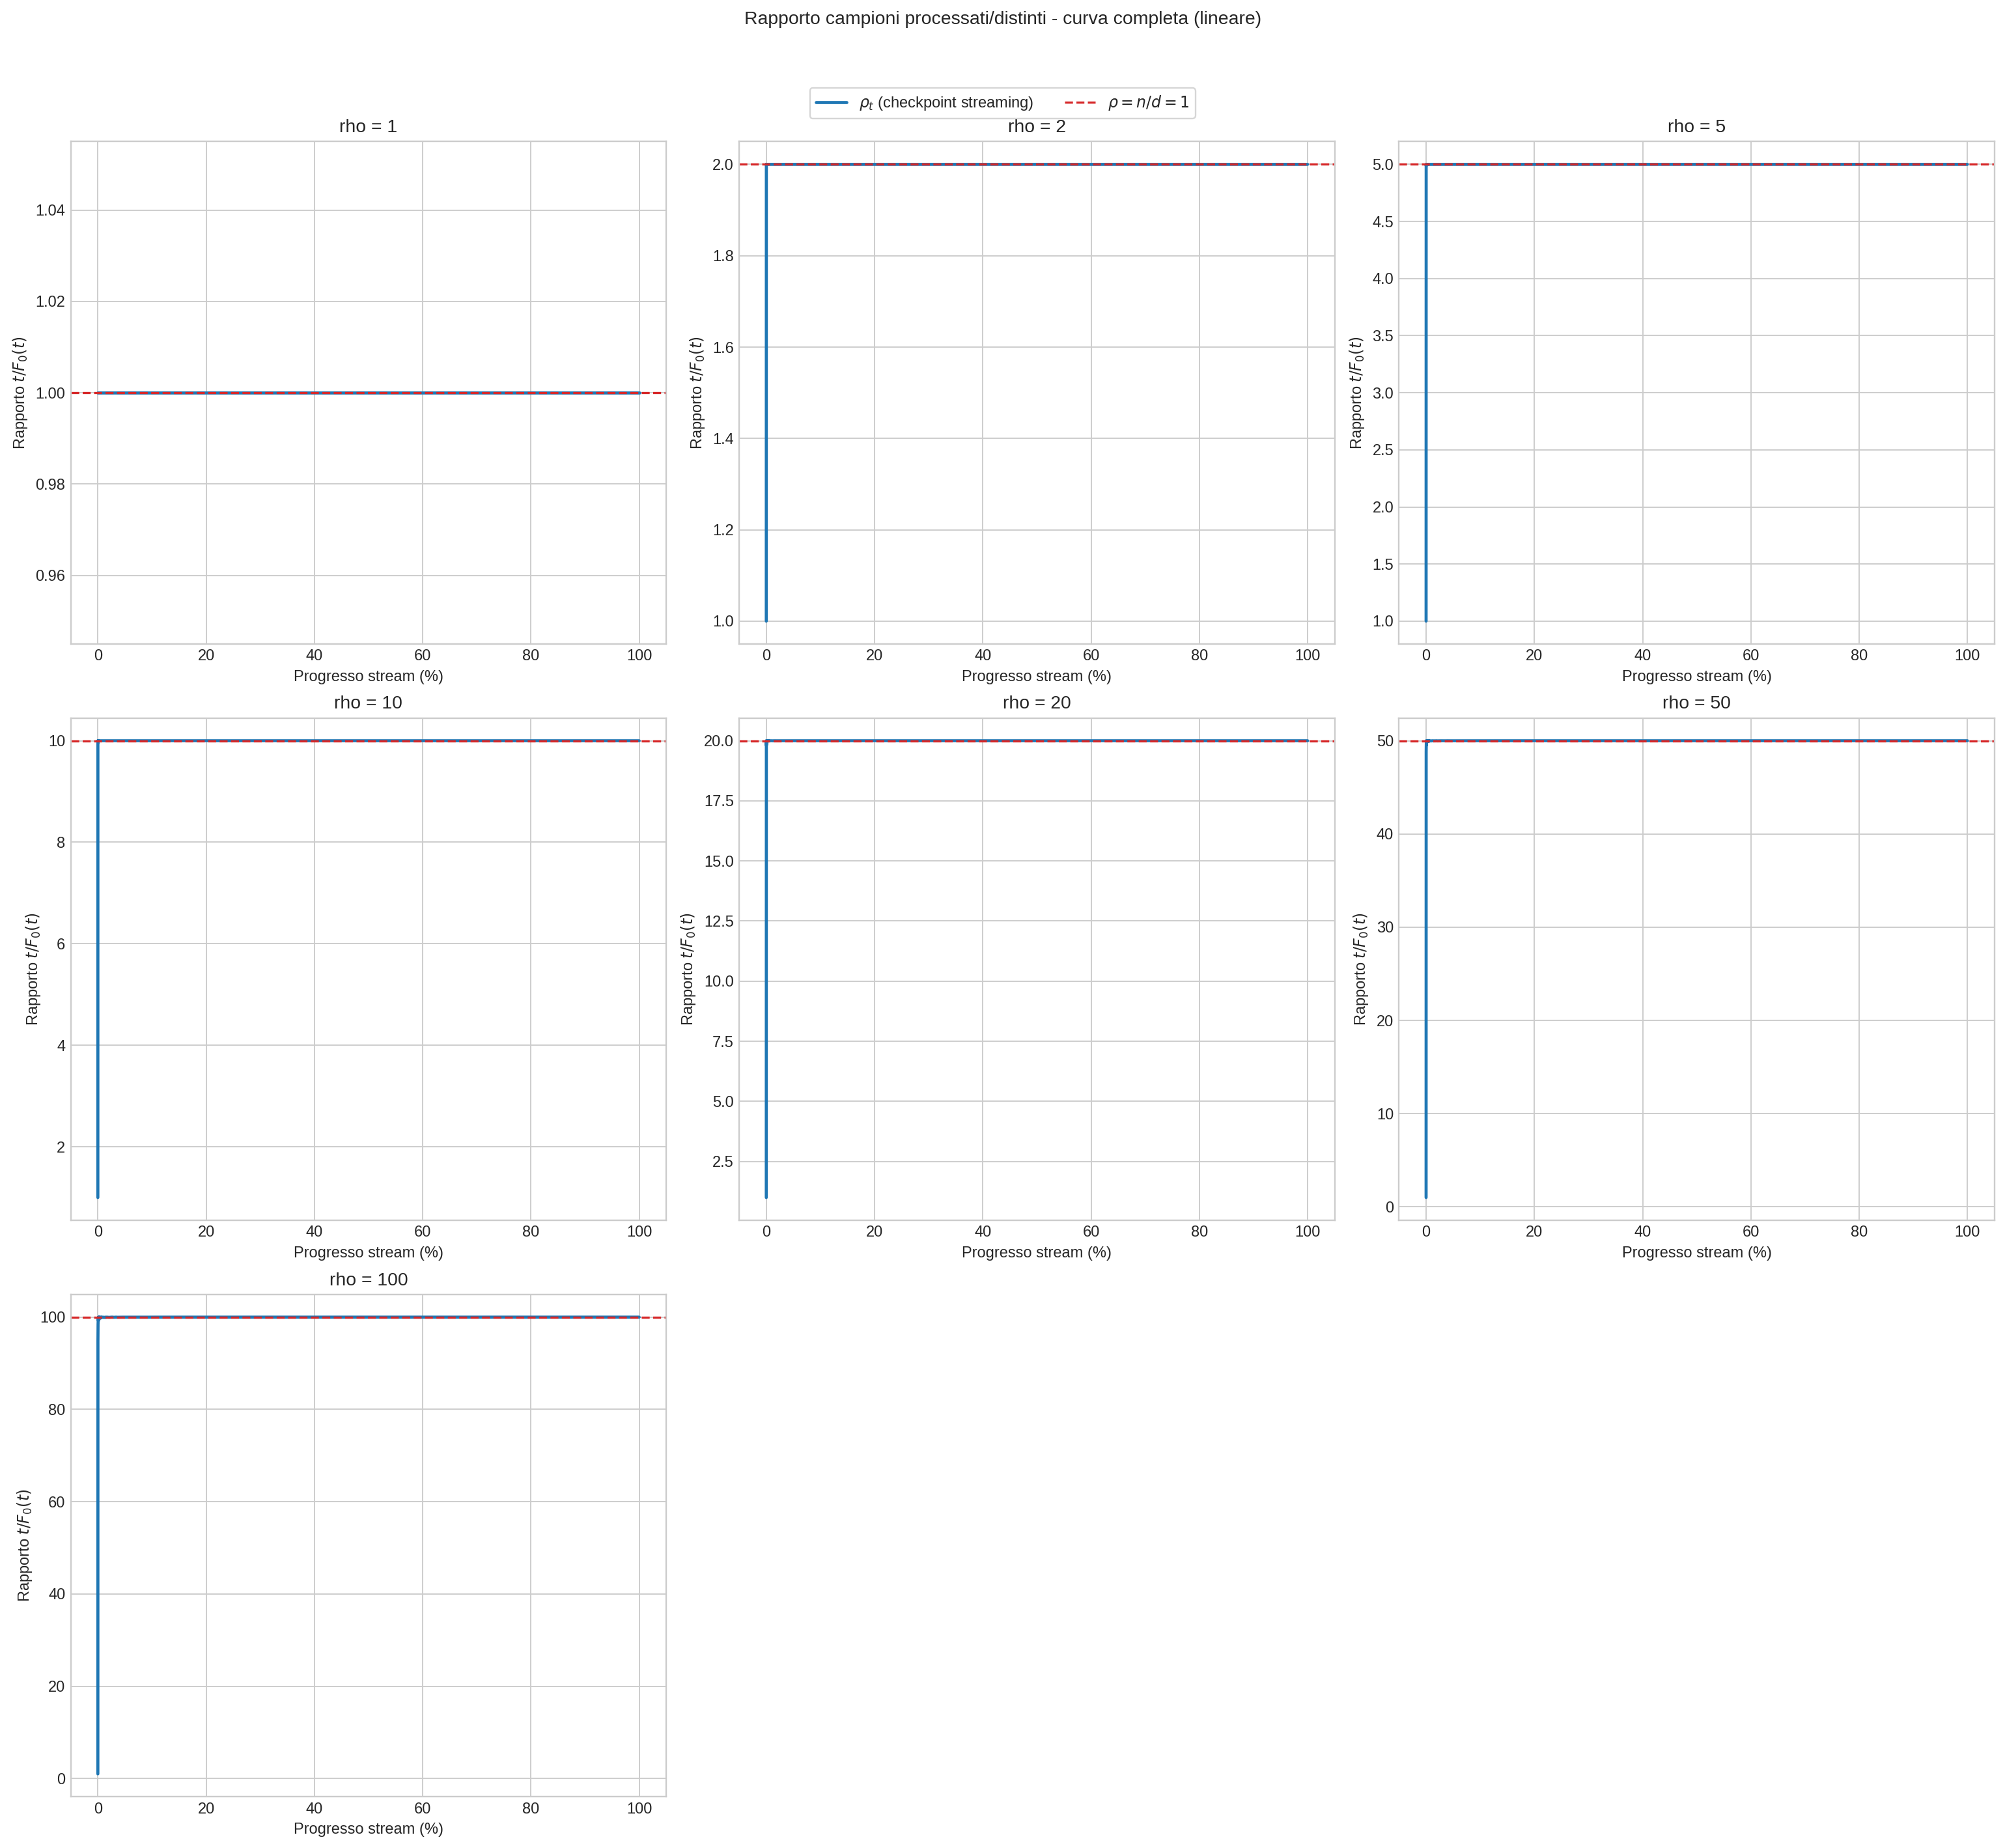
\includegraphics[width=0.96\textwidth]{figures/results/ratio_processed_vs_distinct_streaming_linear.png}
    \caption{Rapporto \(\rho_t=t/F_0(t)\) osservato sui checkpoint di streaming del dataset \texttt{prefix\_constant\_rho}}
    \label{fig:dataset-rho-ratio-linear}
\end{figure}

\begin{figure}[htbp]
    \centering
    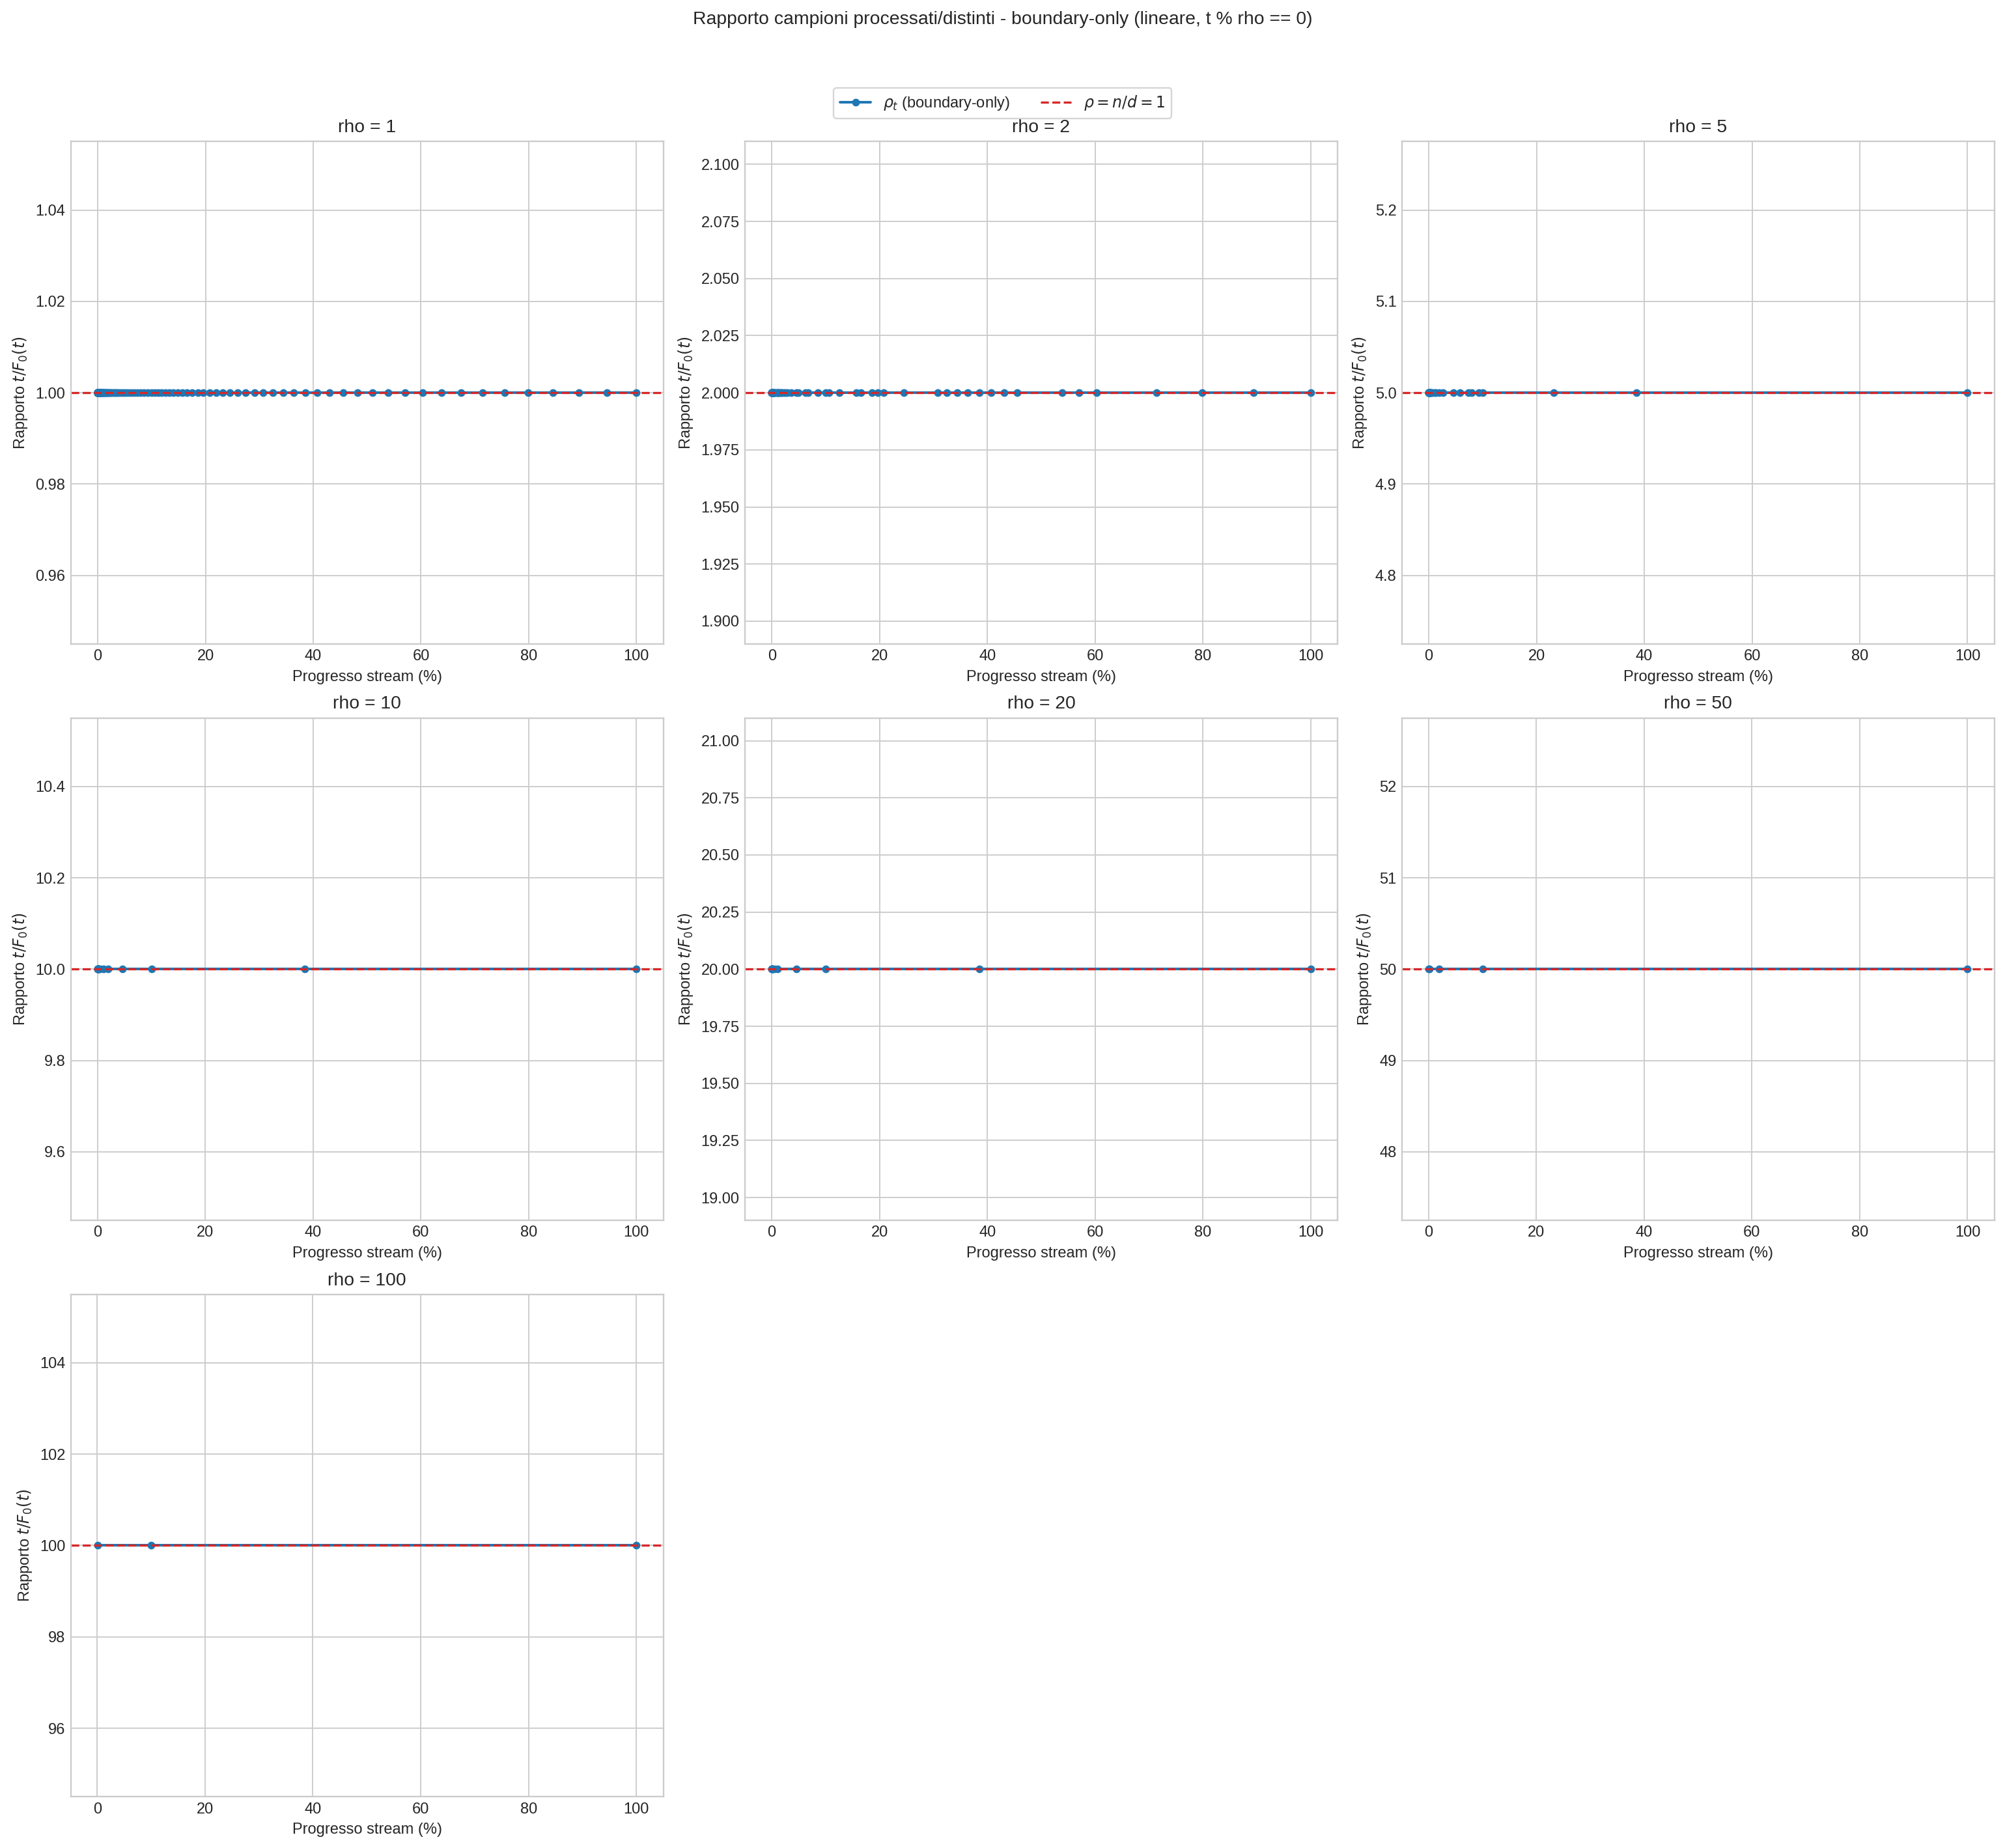
\includegraphics[width=0.96\textwidth]{figures/results/ratio_processed_vs_distinct_streaming_boundary_linear.png}
    \caption{Rapporto \(\rho_t\) osservato ai bordi di blocco, dove per costruzione vale \(\rho_t=\rho\)}
    \label{fig:dataset-rho-ratio-boundary}
\end{figure}

La Figura~\ref{fig:dataset-rho-ratio-linear} mostra la traiettoria completa
osservata ai checkpoint del framework, mentre la
Figura~\ref{fig:dataset-rho-ratio-boundary} evidenzia il comportamento teorico ai
soli multipli di \(\rho\) nei punti di bordo dei blocchi.

\subsection{Riproducibilità del dataset}

La riproducibilità del dataset è garantita da tre elementi:
\begin{itemize}
    \item il seed globale è scritto nell'header del file;
    \item ogni partizione usa un seed derivato in modo deterministico tramite
    \codepath{_derive_partition_seed(seed, partition\_index)};
    \item il generatore è testato esplicitamente in
    \codepath{scripts/tests/test_generate_prefix_constant_rho_dataset.py}.
\end{itemize}

I test verificano la correttezza del formato binario, oltre alla proprietà
\(\sum_t b_t = d\) e alla relazione \(F_0(j\cdot\rho)=j\) insieme alla presenza
di una sola nuova prima occorrenza per blocco e al determinismo del file
prodotto.

\section{Validazione}

La validazione del sistema è distribuita tra test algoritmici, test del
framework e test del generatore del dataset.

\subsection{Test sugli algoritmi}

In \codepath{tests/algorithms} sono presenti test che coprono:
\begin{itemize}
    \item l'accuratezza di base degli algoritmi sui dataset di riferimento;
    \item la validazione dei domini parametrici per HyperLogLog,
    HyperLogLog++ e LogLog;
    \item le proprietà del merge, in particolare commutatività, idempotenza e
    correttezza rispetto al caso omogeneo;
    \item la compatibilità parametrica del merge, con eccezioni esplicite sui
    mismatch non ammessi.
\end{itemize}

Questa parte della validazione è importante perché i limiti di dominio non sono
assunti solo nel testo della tesi, ma difesi direttamente dalle classi concrete.

\subsection{Test del framework}

Il file \codepath{tests/simulation/EvaluationFrameworkTest.cpp} controlla che:
\begin{itemize}
    \item i metadati del framework siano derivati dal dataset e non da valori
    impostati manualmente;
    \item in modalità di flusso il riferimento esatto produca sempre
    \(\hat{F}_0(t)=F_0(t)\) per ogni punto di controllo;
    \item il pianificatore dei punti di controllo copra correttamente il flusso e rispetti il
    budget configurato;
    \item il merge del riferimento esatto coincida con il riferimento seriale;
    \item la serializzazione dei file \texttt{CSV} sia coerente con gli header
    previsti;
    \item il merge eterogeneo copra i casi \texttt{valid},
    \texttt{recoverable} e \texttt{invalid} con le relative strategie.
\end{itemize}

In particolare, i test sul merge eterogeneo verificano quattro regimi:
\begin{itemize}
    \item caso \texttt{valid} con strategia \texttt{direct};
    \item caso \texttt{invalid} con strategia \texttt{reject};
    \item caso \texttt{recoverable} con strategia \texttt{reduce\_then\_merge};
    \item caso \texttt{recoverable} con strategia
    \texttt{unsafe\_naive\_merge}.
\end{itemize}

\subsection{Test del generatore e della catena di esecuzione}

La componente \texttt{Python} è validata da test dedicati sui generatori. In
aggiunta, gli script di orchestrazione costruiscono payload di comandi per la
riga di comando in modo deterministico, fissando namespace dei risultati,
funzioni di hash e griglie parametriche. Anche questa scelta contribuisce alla
riproducibilità complessiva della catena di esecuzione.

\section{Considerazioni progettuali}

La struttura implementativa adottata in questa tesi riflette una scelta precisa:
mettere al centro non un singolo algoritmo, ma la possibilità di confrontare
famiglie algoritmiche diverse in un ambiente coerente.

Dal punto di vista algoritmico, la scelta più importante è l'uso di una
interfaccia comune con validazione rigorosa dei domini e con merge esposto come
operazione di primo livello. Questo rende confrontabili gli sketch non solo in
termini di accuratezza, ma anche in termini di semantica operativa.

Dal punto di vista dell'hashing, la decisione cruciale è stata trattare la
funzione di hash come dipendenza esplicita e non come dettaglio nascosto delle
classi concrete. Questa scelta è ciò che rende possibile, nel capitolo
sperimentale, distinguere in modo netto tra casi omogenei, casi recuperabili e
casi non validi.

Dal punto di vista del framework, la scelta più utile è stata separare dataset,
coordinamento, valutazione e serializzazione. In questo modo gli esperimenti del
capitolo sperimentale non sono stati costruiti come script ad hoc, ma come
istanze diverse della stessa infrastruttura.

Infine, la presenza del dataset \texttt{prefix\_constant\_rho} con bitset di
verità integrato chiude il cerchio metodologico: gli algoritmi sono implementati
come componenti indipendenti, l'hashing è controllabile, il framework li misura
in modo uniforme e il dataset fornisce il riferimento esatto necessario per
leggere correttamente i risultati.

    \chapter{Risultati sperimentali}
\label{chp:risultati_nuovo}

I risultati sperimentali raccolti seguono la stessa progressione con cui è
stato costruito il lavoro. Si parte dalla verifica del
contesto sperimentale, cioè dal controllo empirico del dataset
\texttt{prefix\_constant\_rho} e dalla scelta di un seed stabile per gli
esperimenti successivi. Su questa base vengono poi confrontati gli algoritmi, 
osservando come evolve la stima lungo i prefissi e come
essa cambi al variare del rapporto tra elementi processati e distinti e del
parametro di precisione.

La seconda parte è dedicata al merge di sketch. Il punto di partenza è il caso
omogeneo, usato come controllo di correttezza dell'infrastruttura. Si passa poi
ai casi eterogenei, distinguendo tra situazioni \texttt{valid},
\texttt{invalid} e \texttt{recoverable}. Gli esperimenti su funzioni di hash
diverse e su mismatch di precisione servono da un lato a verificare quanto
emerso nella letteratura, dall'altro a mostrare che il framework costruito
consente di studiare in modo sistematico casi di merge non ideali.

\paragraph{Ambiente di test}
I risultati sono stati ottenuti su una workstation con processore AMD Ryzen 7
9700X, 32 GB di memoria DDR5 e unità a stato solido NVMe da 1 TB, con sistema
operativo CachyOS e ambiente grafico COSMIC.

La catena di compilazione utilizzata è:
\begin{itemize}[noitemsep]
    \item CMake 4.3.0;
    \item Clang 22.1.1;
    \item target \texttt{x86\_64-pc-linux-gnu}.
\end{itemize}

\section{Validazione del contesto sperimentale}

Prima di confrontare gli algoritmi è necessario verificare che il contesto di
prova sia coerente con le ipotesi alla base degli esperimenti successivi. La
sezione raccoglie quindi i controlli preliminari sul dataset utilizzato e sulla
scelta del seed mantenuto nelle esecuzioni principali.

\subsection{Verifica empirica del dataset a prefisso costante}

Gli esperimenti usano il dataset a prefisso costante con le seguenti configurazioni:
\[
n=10^7,\qquad p=50,\qquad seed=21041998,\qquad
d \in \{10^5,2\cdot 10^5,5\cdot 10^5,10^6,2\cdot 10^6,5\cdot 10^6,10^7\}
\]
\[
\rho=\frac{n}{d}\in\{100,50,20,10,5,2,1\}
\]
I sette valori di \(\rho\) corrispondono ai rapporti tra elementi processati e
distinti usati nel resto del capitolo.

La validazione empirica del comportamento del dataset è mostrata nelle
Figure~\ref{fig:ch5-dataset-rho-ratio-linear} e
\ref{fig:ch5-dataset-rho-ratio-boundary}.
La prima figura mostra il rapporto \(\rho_t=t/F_0(t)\) sui punti di controllo
effettivamente usati nella modalità di flusso, mentre la seconda isola i soli
punti di bordo dei blocchi, nei quali il rapporto assume il valore costante
previsto dalla costruzione.

Dalle figure si osserva che il comportamento atteso è rispettato. All'interno
  di ciascun blocco la cardinalità distinta non cresce, perché non vengono
  introdotte nuove prime occorrenze, mentre ai bordi di blocco essa aumenta di una
  sola unità. Ne segue che il rapporto \(\rho_t=t/F_0(t)\) assume il valore
  teorico \(\rho\) esattamente nei punti \(t=j\cdot\rho\), in accordo con la
  costruzione del dataset.

\begin{figure}[htbp]
    \centering
    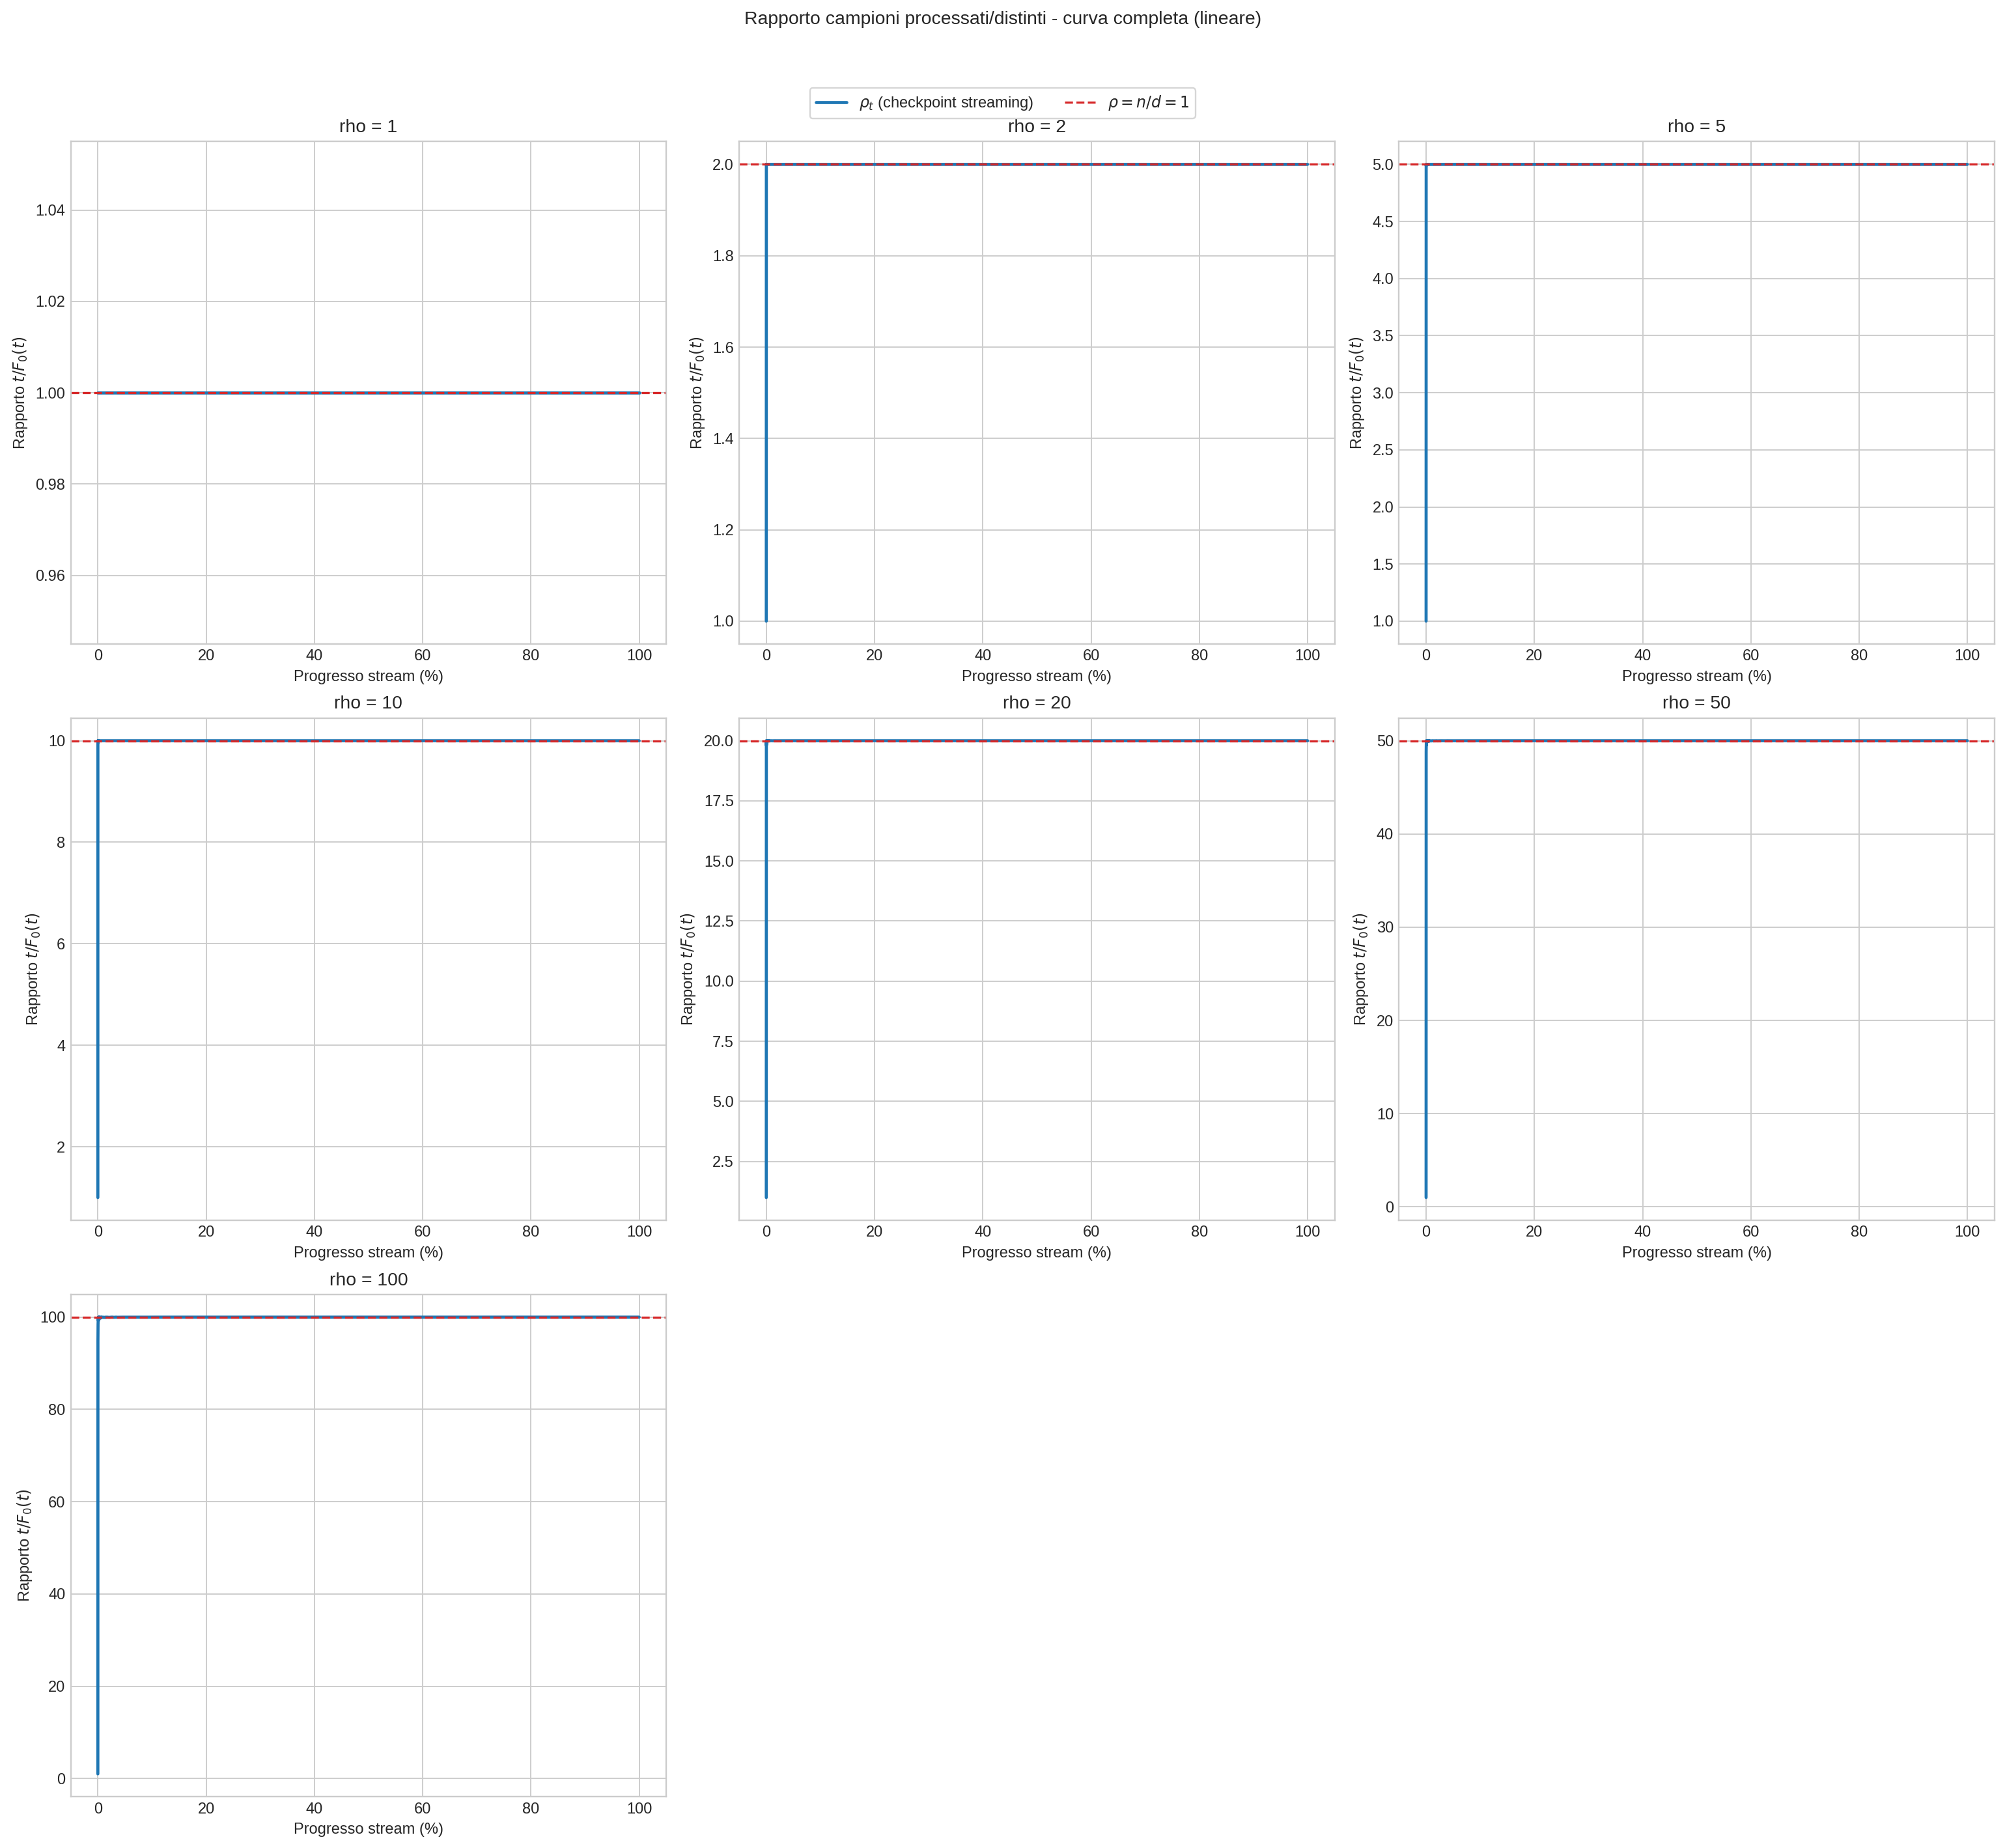
\includegraphics[width=0.96\textwidth]{figures/results/ratio_processed_vs_distinct_streaming_linear.png}
    \caption{Rapporto \(\rho_t=t/F_0(t)\) osservato ai checkpoint del dataset}
    \label{fig:ch5-dataset-rho-ratio-linear}
\end{figure}

\begin{figure}[htbp]
    \centering
    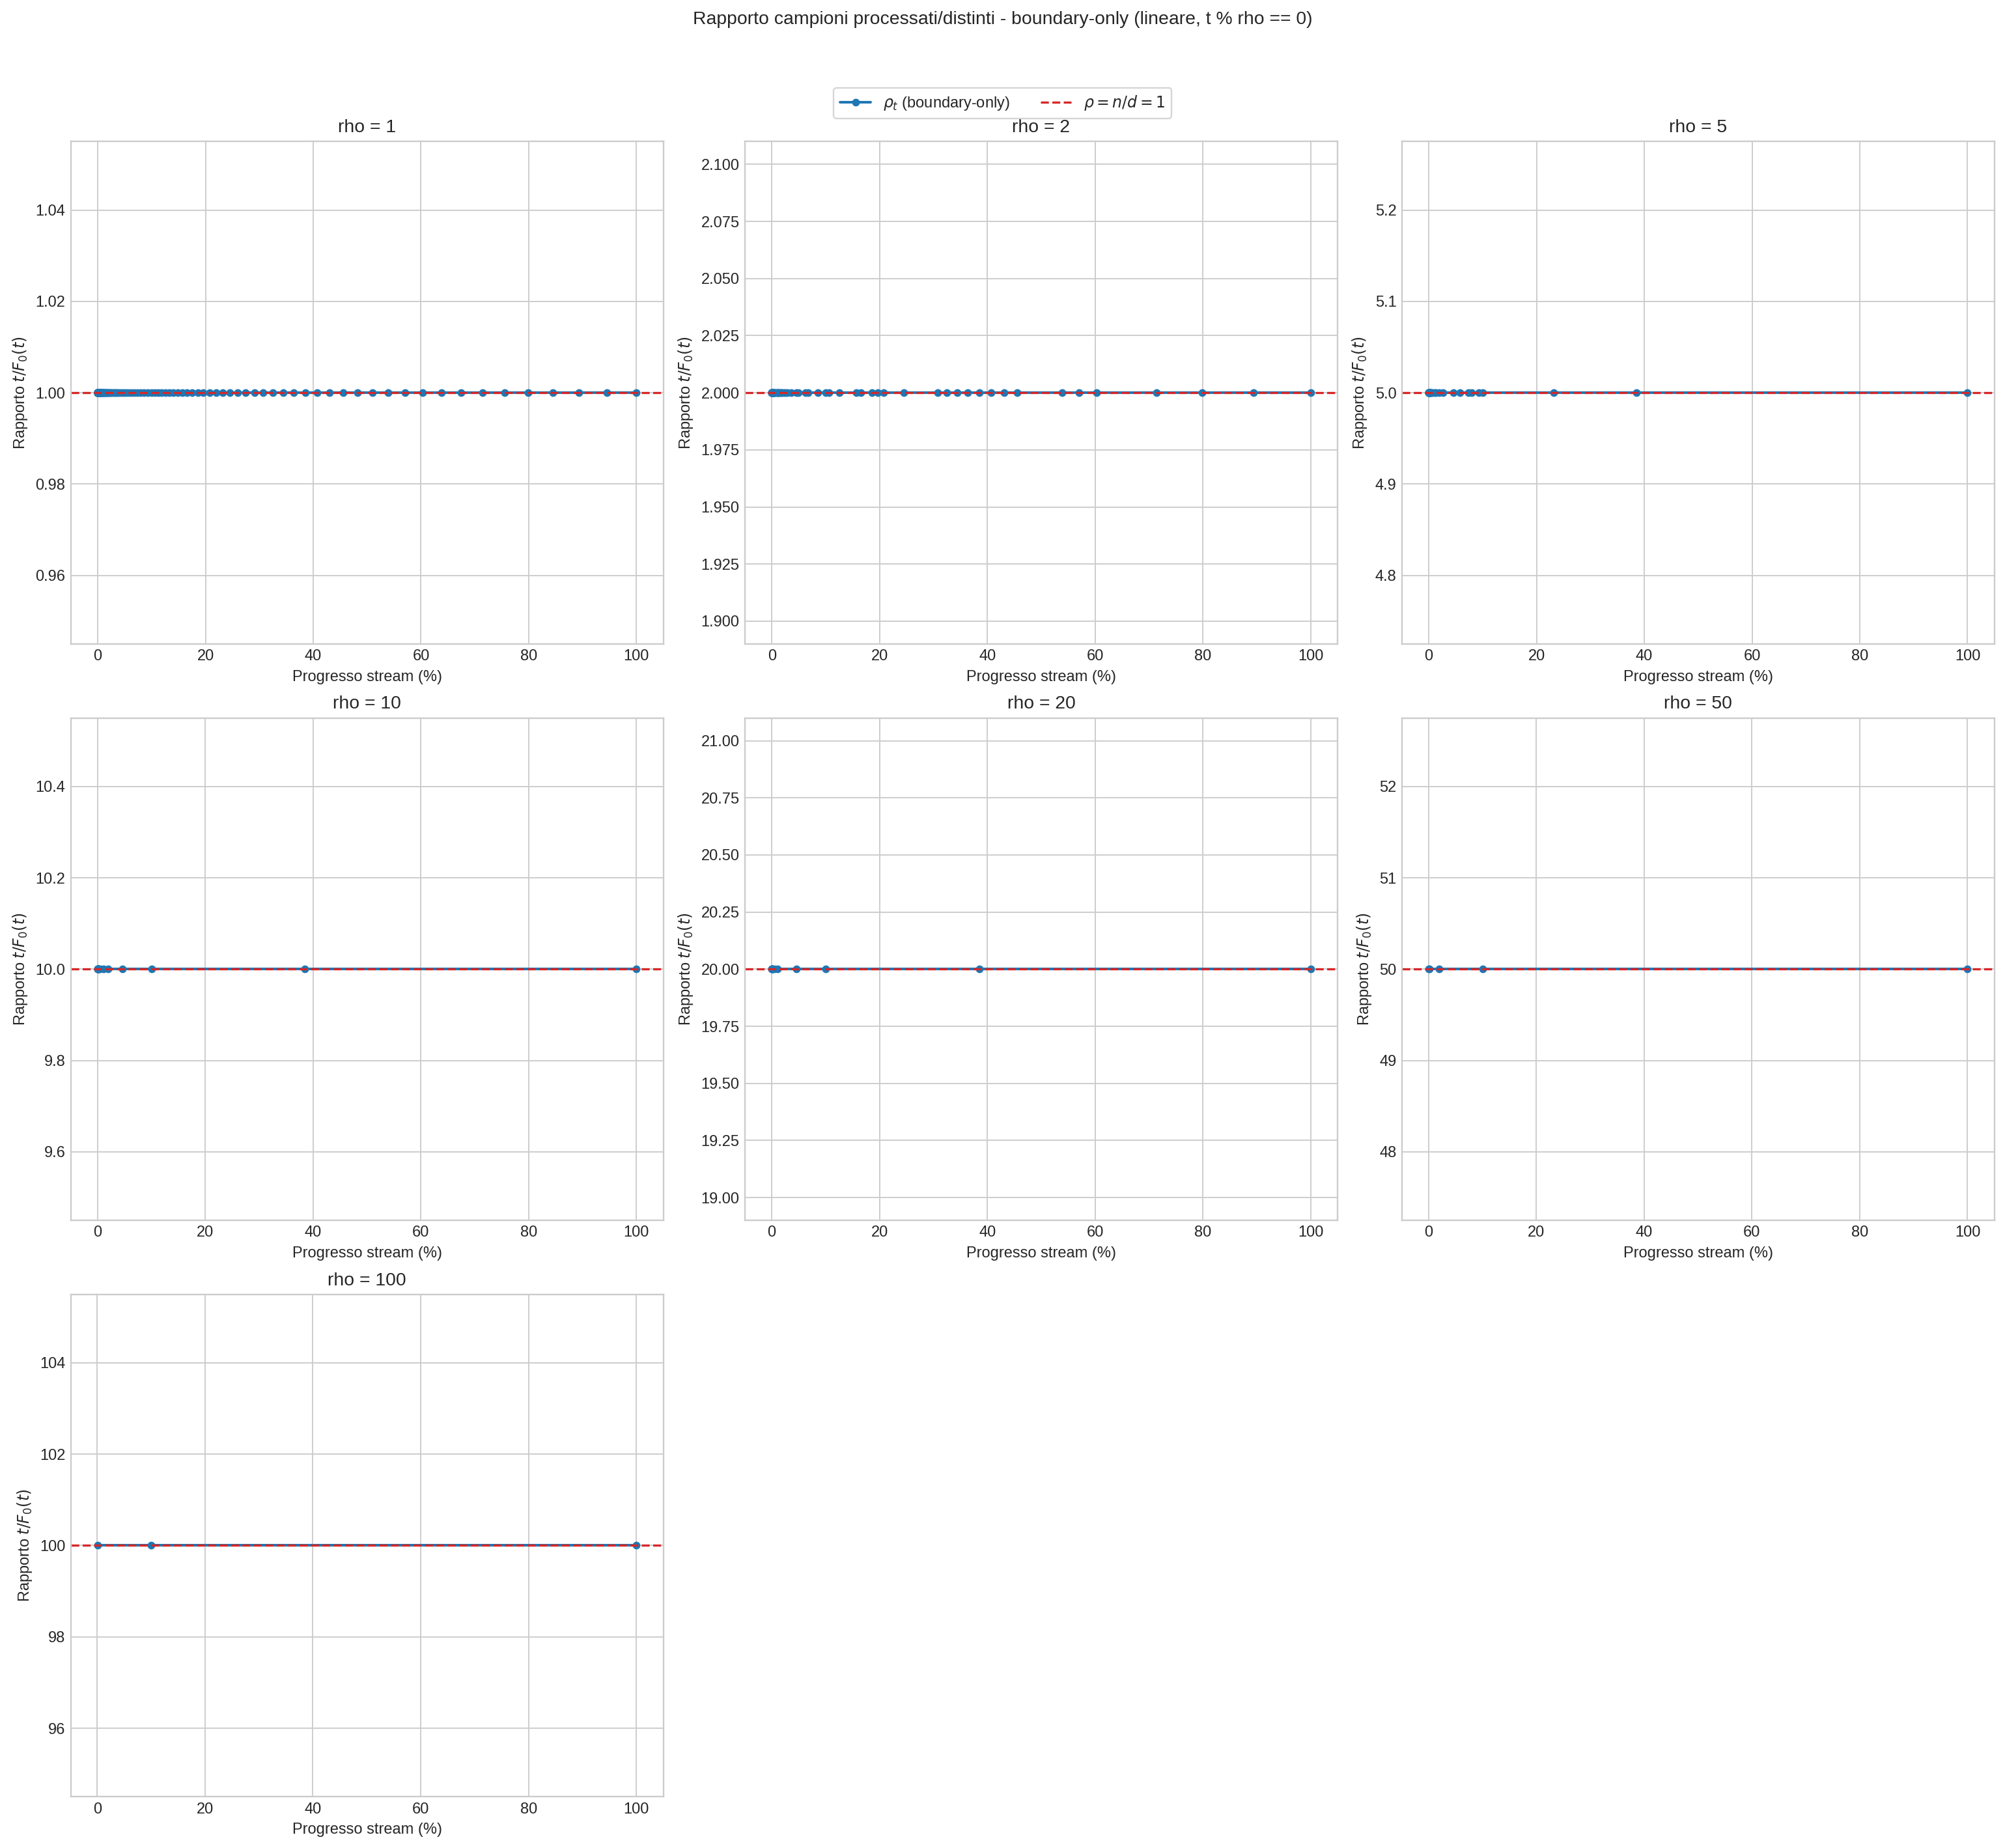
\includegraphics[width=0.96\textwidth]{figures/results/ratio_processed_vs_distinct_streaming_boundary_linear.png}
    \caption{Rapporto \(\rho_t\) osservato ai bordi di blocco}
    \label{fig:ch5-dataset-rho-ratio-boundary}
\end{figure}

\subsection{Scelta del seed}
Una verifica preliminare, svolta nelle prime iterazioni degli esperimenti, ha
indicato che l'effetto del seed resta ininfluente rispetto alle differenze tra
algoritmi e tra le varie modalit\`a di merge.

Non sono stati fatti confronti con pi\`u dataset con seed diversi ma stessi parametri
anche per una questione di spazio richiesto. 

Ogni dataset pesa nell'ordine dei 2 GB dopo la compressione, per 50 milioni di elementi.
Le configurazioni testate sono tante e sarebbe diventato arduo testarle tutte.

Per questo motivo gli esperimenti principali fissano un seed unico pari a
\(21041998\).

\section{Esperimenti sugli algoritmi}
Gli esperimenti sugli algoritmi sono organizzati in due gruppi complementari.
  Il primo ha lo scopo di osservare come cambia la qualità della stima al variare
  della cardinalità reale del prefisso e del rapporto tra elementi processati e
  distinti. L'interesse non è limitato al solo errore medio, ma comprende anche
  la dispersione della stima, così da distinguere chiaramente tra fenomeni di
  bias e fenomeni di scarsa robustezza.

  Per isolare questi effetti sono state considerate due viste del problema. Nella
  prima si fissa il rapporto
  \[
  \rho=\frac{n}{d}
  \]
  e si osserva la stima in funzione della cardinalità reale del prefisso. Nella
  seconda si fissano valori obiettivo della cardinalità reale e si studia la
  stima in funzione del rapporto medio di ripetizione del prefisso,
  \[
  \rho_t=\frac{t}{F_0(t)}
  \]
  in modo da separare, per quanto possibile, l'effetto della crescita dei distinti
  da quello delle ripetizioni medie.

  Il secondo gruppo di esperimenti mantiene fisso il contesto di esecuzione e
  varia invece il parametro interno di precisione di ciascun algoritmo. Questa
  analisi serve a capire non solo quale algoritmo sia più accurato nel complesso,
  ma anche quanto il suo comportamento dipenda dalla scelta del parametro e se il
  miglioramento ottenuto all'aumentare delle risorse sia regolare oppure no.
\subsection{Configurazione utilizzata}

Gli esperimenti usano il dataset:
\begin{center}
\small
\codepath{datasets/prefix_constant_rho/dataset_n_10000000_d_<d>_p_50_s_21041998.bin}
\end{center}

I risultati sono salvati in:
\begin{center}
\small
\codepath{results/prefix_constant_rho/streaming/.../results_streaming.csv}
\end{center}

Le metriche principali osservate sono:
\begin{itemize}
    \item cardinalità reale del prefisso \(\,F_0(t)\,\) in
    \texttt{f0\_mean\_t};
    \item stima media \(\,\hat{F}_0(t)\,\) in \texttt{f0\_hat\_mean\_t};
    \item dispersione della stima con bande \(\mu \pm \sigma\);
    \item errore relativo medio ai punti finali osservati, usato come sintesi
    comparativa tra algoritmi.
\end{itemize}

\subsection{Analisi della robustezza degli algoritmi}
L'obiettivo di questa parte è capire rispetto a quali parametri gli algoritmi si
  comportino bene o male. I due parametri considerati sono il numero reale di
  elementi distinti osservati in un prefisso e il rapporto tra elementi processati
  e distinti, cioè il numero medio di ripetizioni del prefisso.

  L'analisi tiene conto di due aspetti diversi della qualità della stima. Il primo
  è il bias, cioè lo scostamento sistematico tra il valore medio stimato e il
  numero corretto di elementi distinti. Il secondo è la robustezza, cioè la
  dispersione della stima attorno al suo valore medio: uno stimatore può anche
  essere corretto in media, ma restare comunque molto sensibile al rumore e quindi
  presentare una varianza elevata. Per questa ragione, nei grafici vengono
  mostrati insieme il valore medio della stima e la sua dispersione.

  Per studiare separatamente la dipendenza da questi due parametri, sono stati
  adottati due protocolli sperimentali distinti.

  Nel primo caso, chiamato per facilit\`a caso $A$, si fissa il rapporto
  \[
  \rho=\frac{n}{d}
  \]
  e si osserva l'andamento della stima al variare del numero reale di elementi
  distinti presenti nel prefisso. In questo modo si analizza come cambino bias e
  dispersione a parità di ripetizione media.

  Nel secondo caso, chiamato caso $B$, si fissano alcuni valori target della cardinalità reale e si
  osserva la stima in funzione del rapporto medio di ripetizione del prefisso,
  calcolato come
  \[
  \rho_t=\frac{t}{F_0(t)}
  \]
  Questa scelta è necessaria perché usare il numero grezzo di elementi processati
  come ascissa introdurrebbe implicitamente anche una dipendenza dal numero di
  elementi distinti. Il rapporto \(\rho_t\) permette invece di isolare meglio
  l'effetto delle ripetizioni medie sul comportamento degli algoritmi.
\subsubsection{Stima in funzione della cardinalità reale del prefisso}
\label{sec:ch5-streaming-f0}

Questa analisi corrisponde ai grafici precedentemente indicati come
analisi del caso A.
L'ascissa riporta la cardinalità reale \(F_0(t)\), l'ordinata la stima
\(\hat{F}_0(t)\), e i pannelli sono separati per ciascun valore di \(\rho\).

\begin{figure}[p]
    \centering
    \begin{subfigure}[t]{0.49\textwidth}
        \centering
        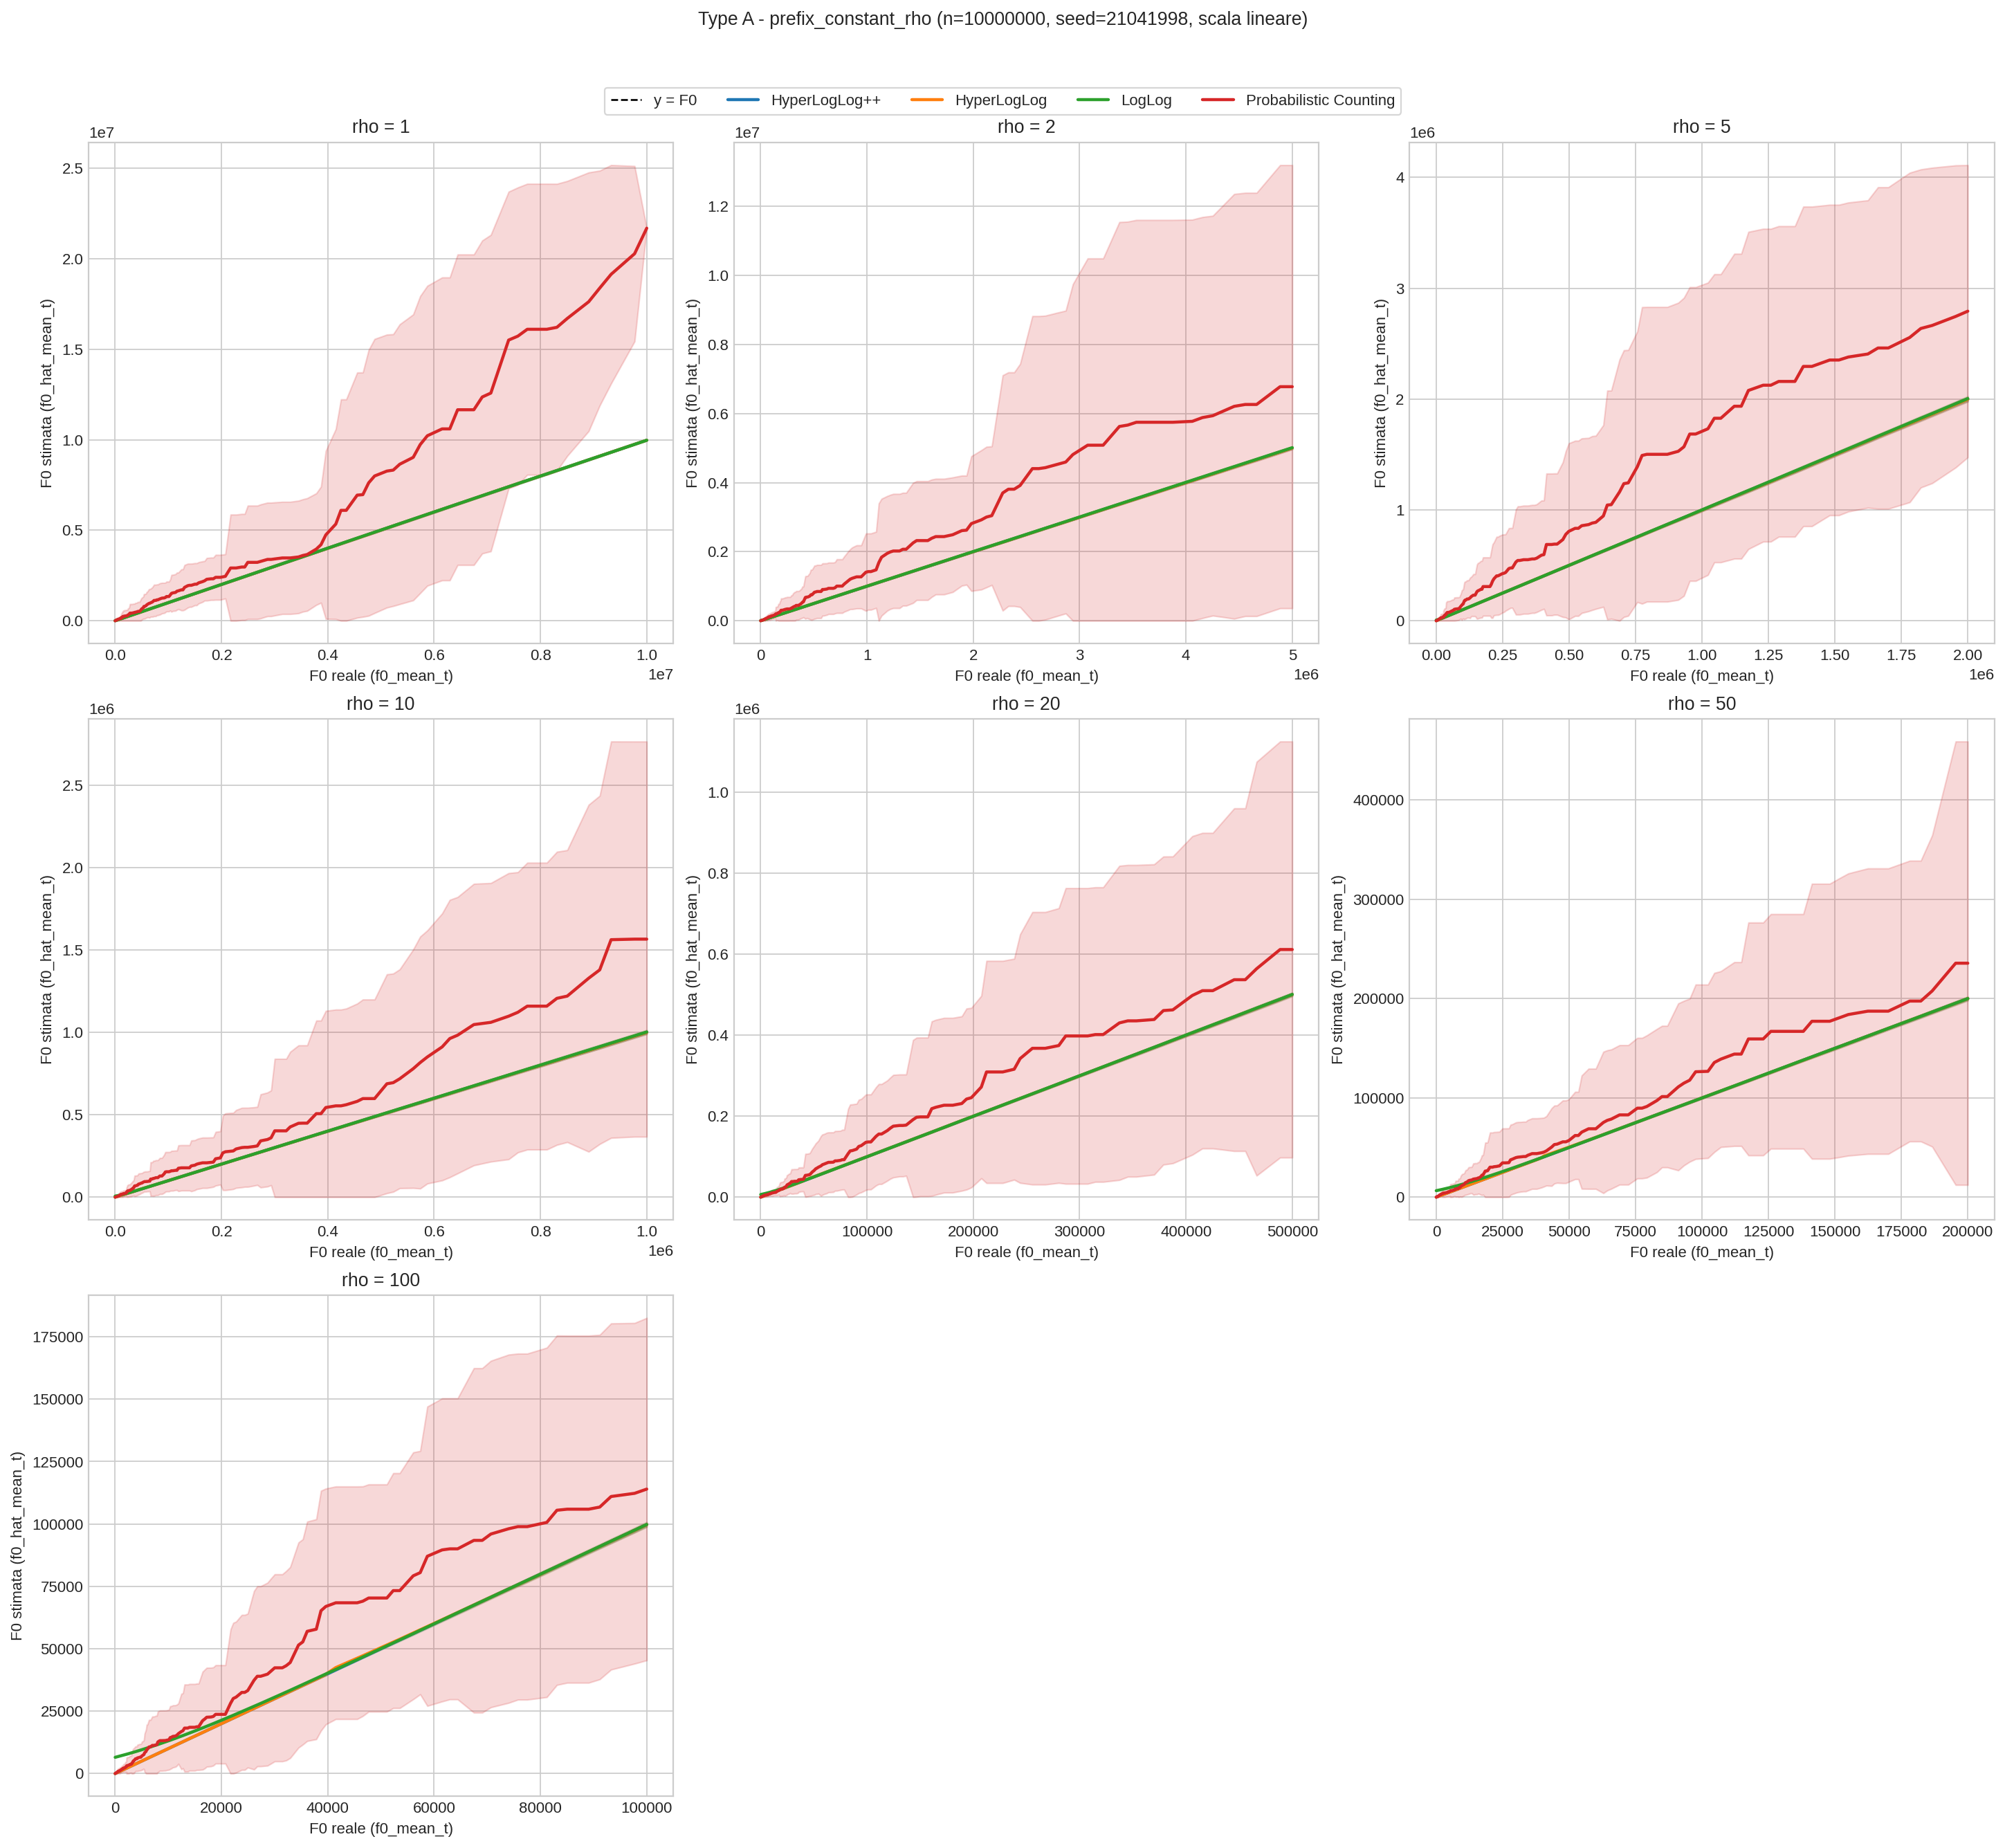
\includegraphics[width=\linewidth]{figures/results/typeA_prefix_constant_rho_linear.png}
        \caption{Scala lineare}
        \label{fig:ch5-stream-f0-all-linear}
    \end{subfigure}
    \hfill
    \begin{subfigure}[t]{0.49\textwidth}
        \centering
        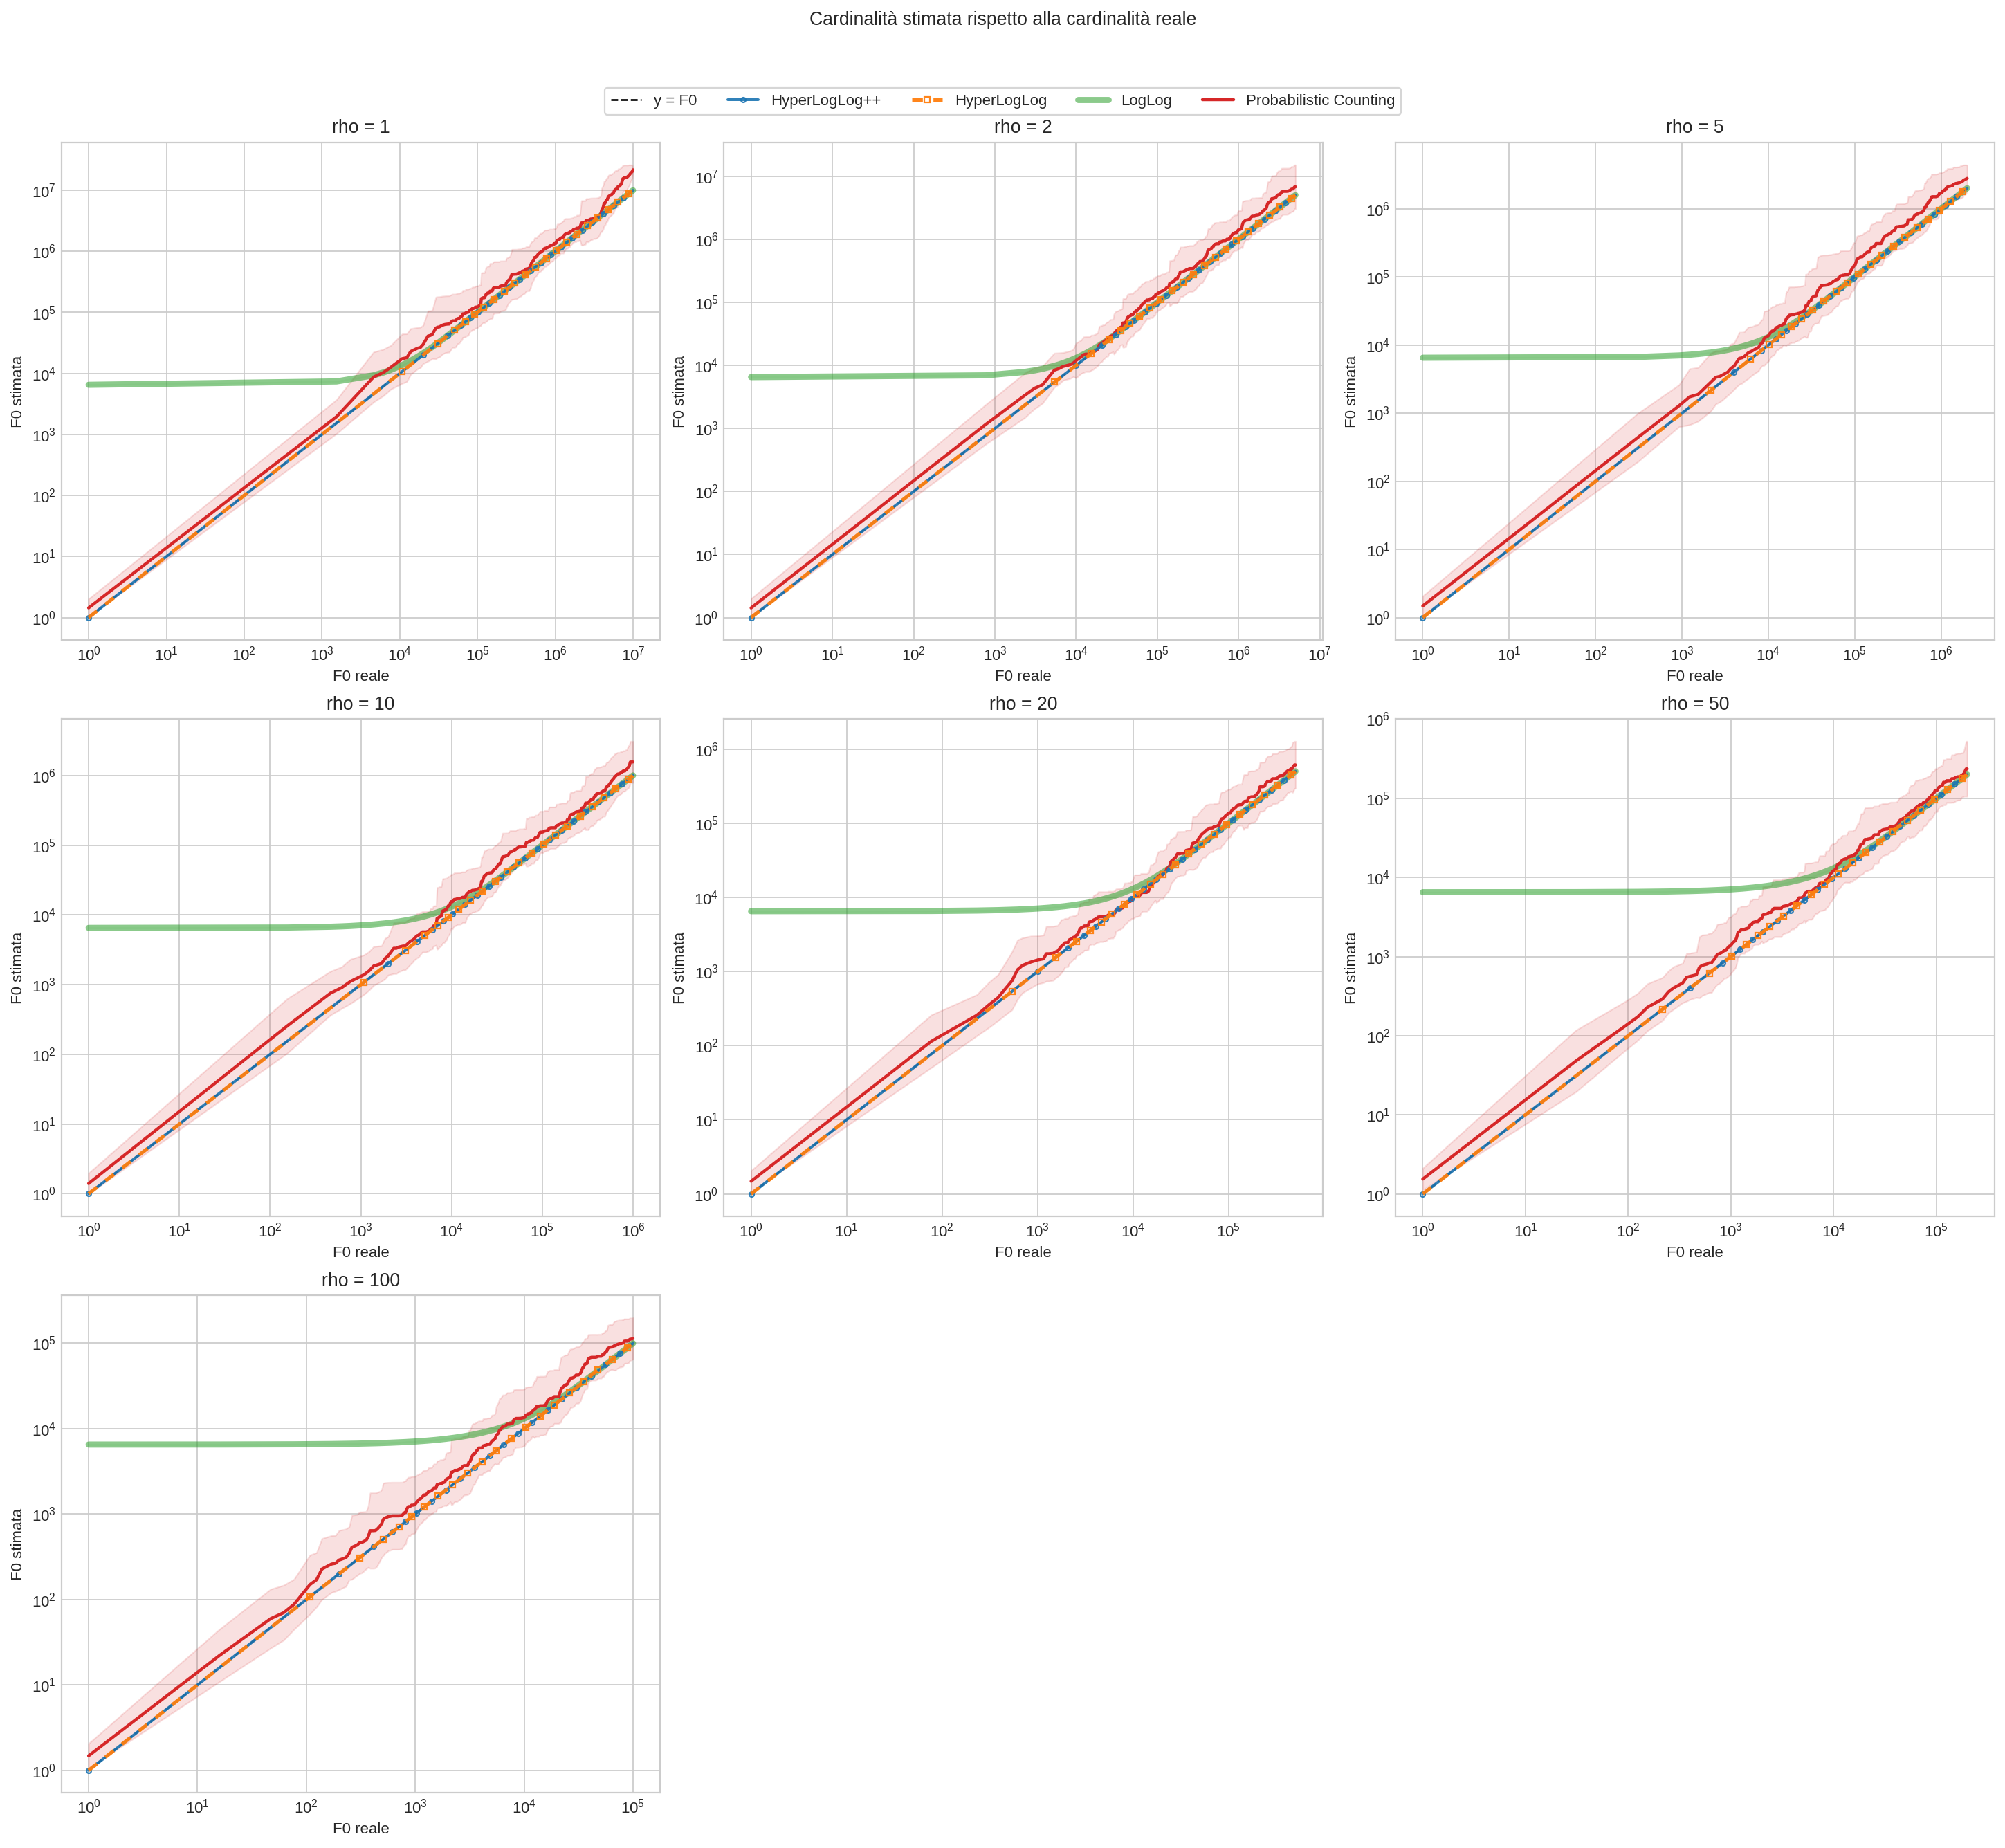
\includegraphics[width=\linewidth]{figures/results/typeA_prefix_constant_rho_loglog.png}
        \caption{Scala logaritmica}
        \label{fig:ch5-stream-f0-all-loglog}
    \end{subfigure}
    \caption{Stima rispetto alla cardinalità reale del prefisso, tutti gli algoritmi}
    \label{fig:ch5-stream-f0-all}
\end{figure}

\begin{figure}[p]
    \centering
    \begin{subfigure}[t]{0.49\textwidth}
        \centering
        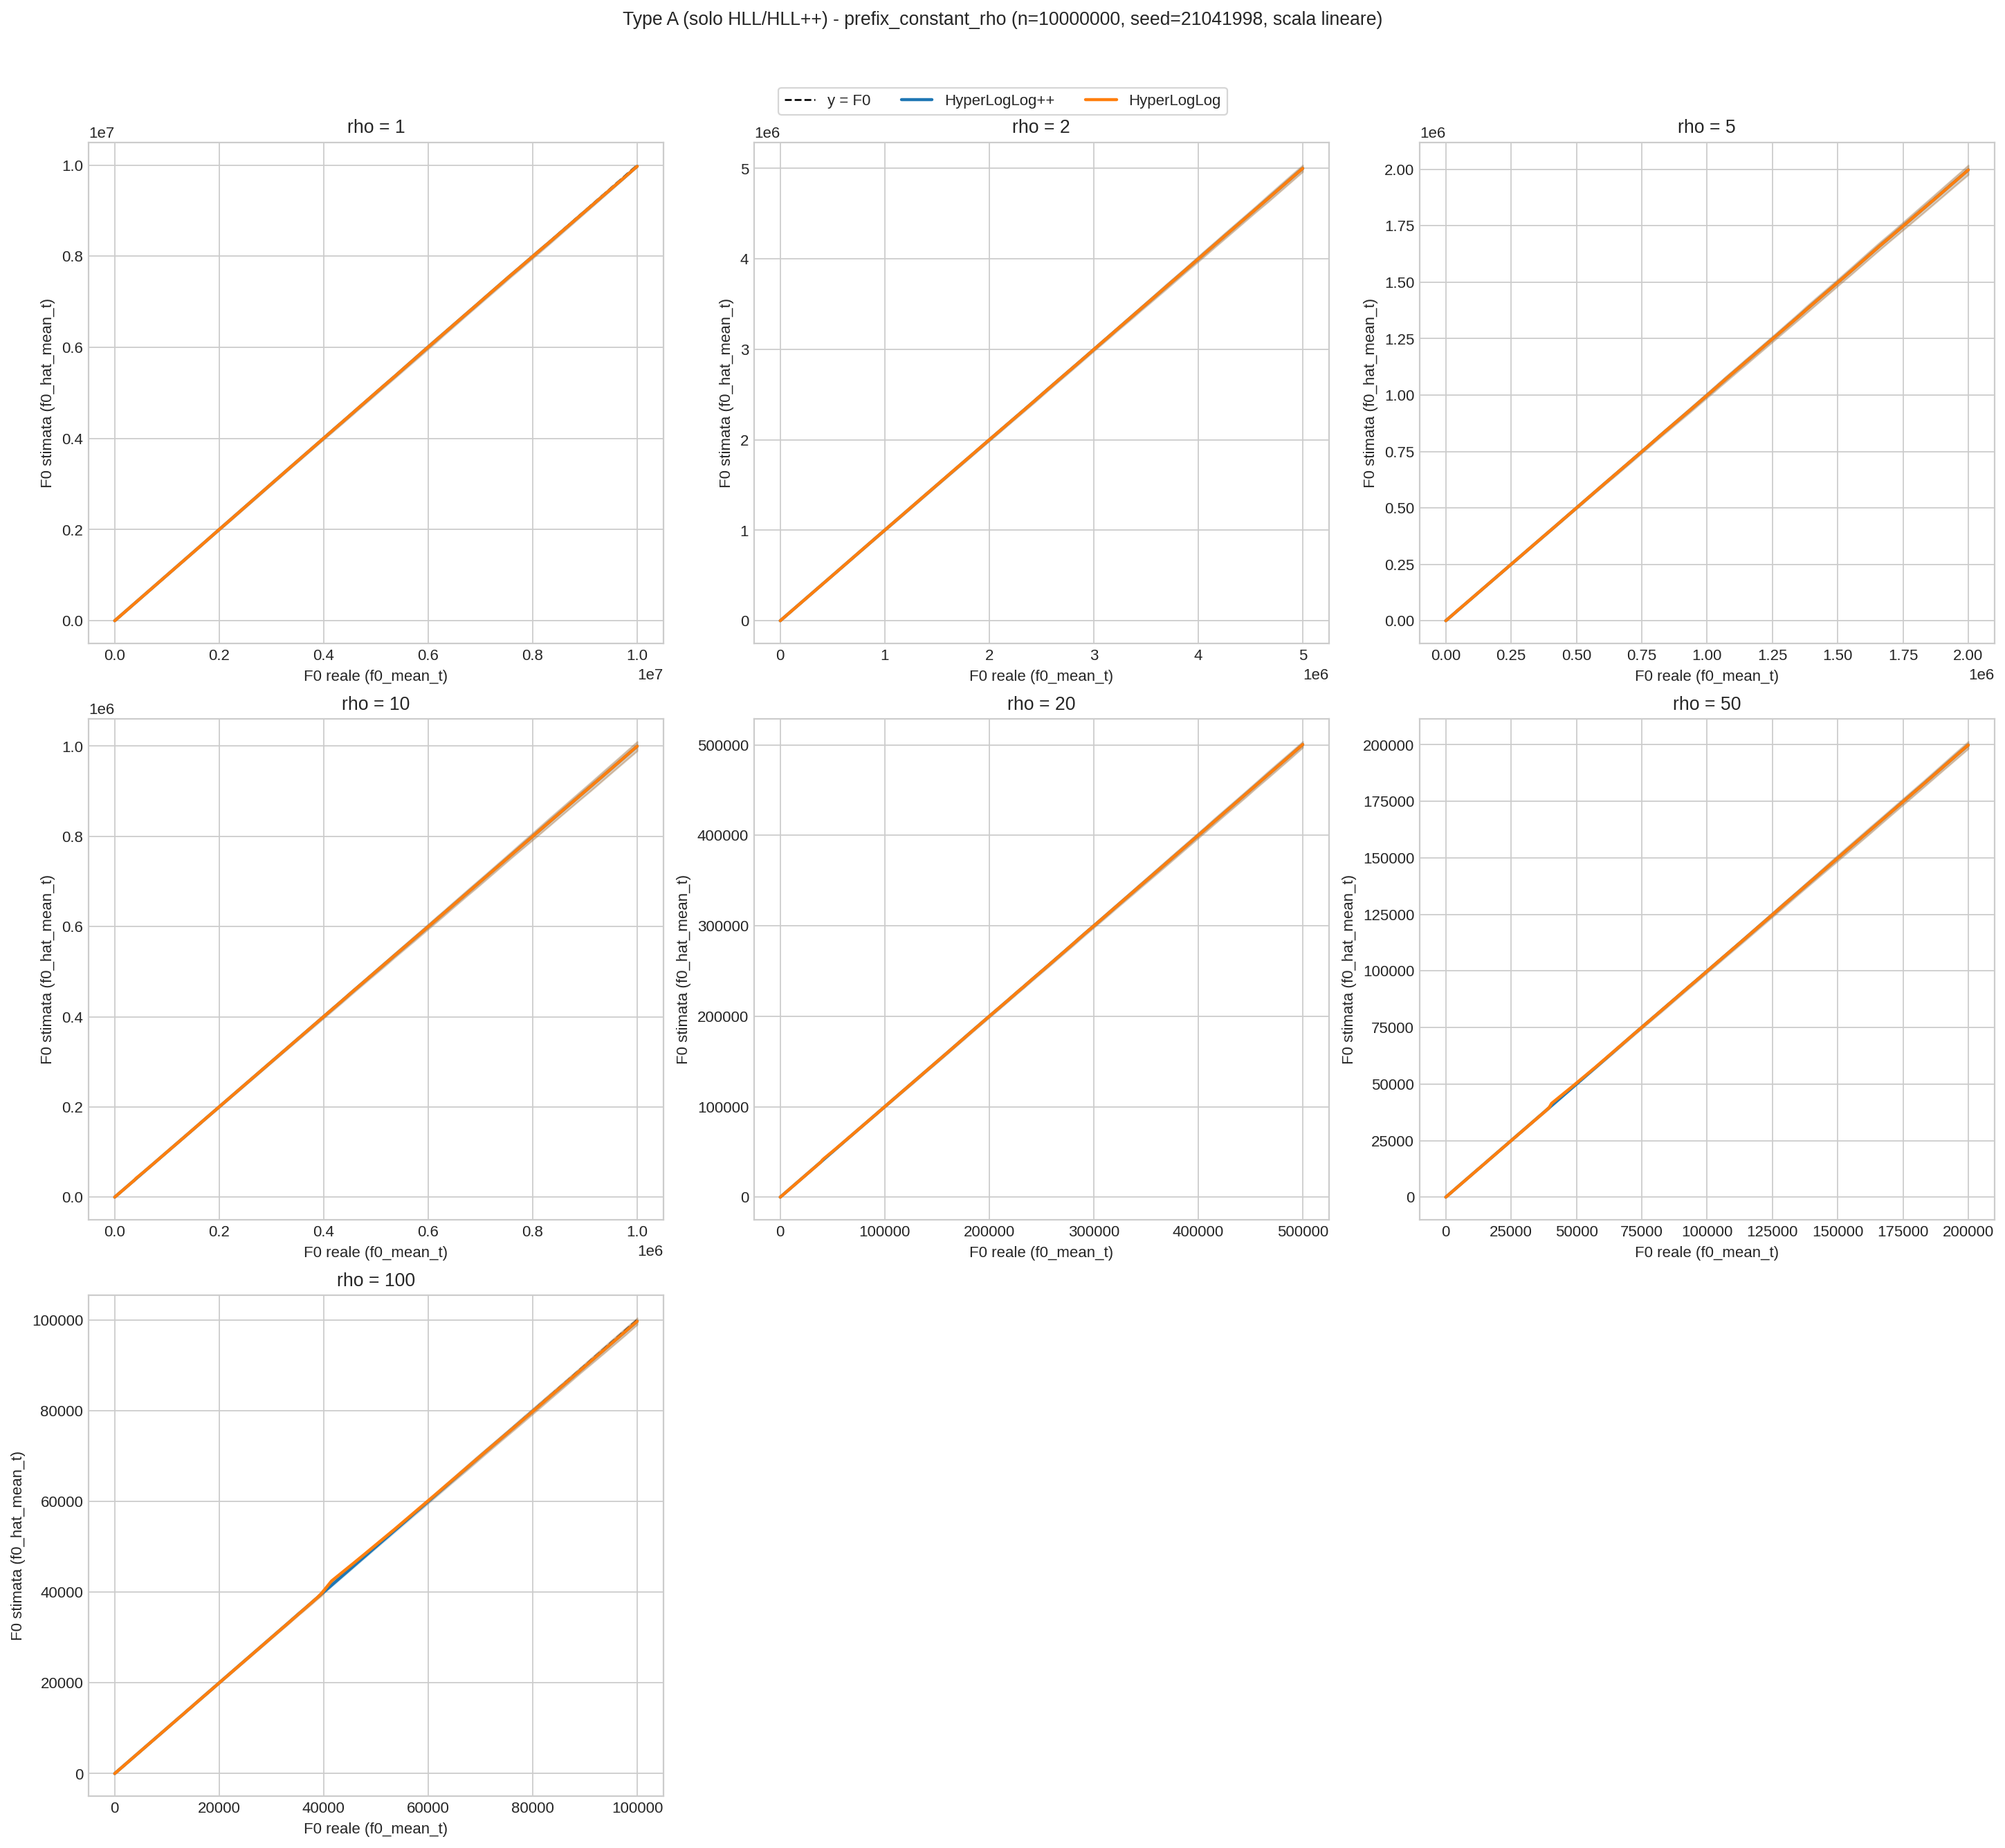
\includegraphics[width=\linewidth]{figures/results/typeA_prefix_constant_rho_hll_hllpp_linear.png}
        \caption{Scala lineare}
        \label{fig:ch5-stream-f0-hll-linear}
    \end{subfigure}
    \hfill
    \begin{subfigure}[t]{0.49\textwidth}
        \centering
        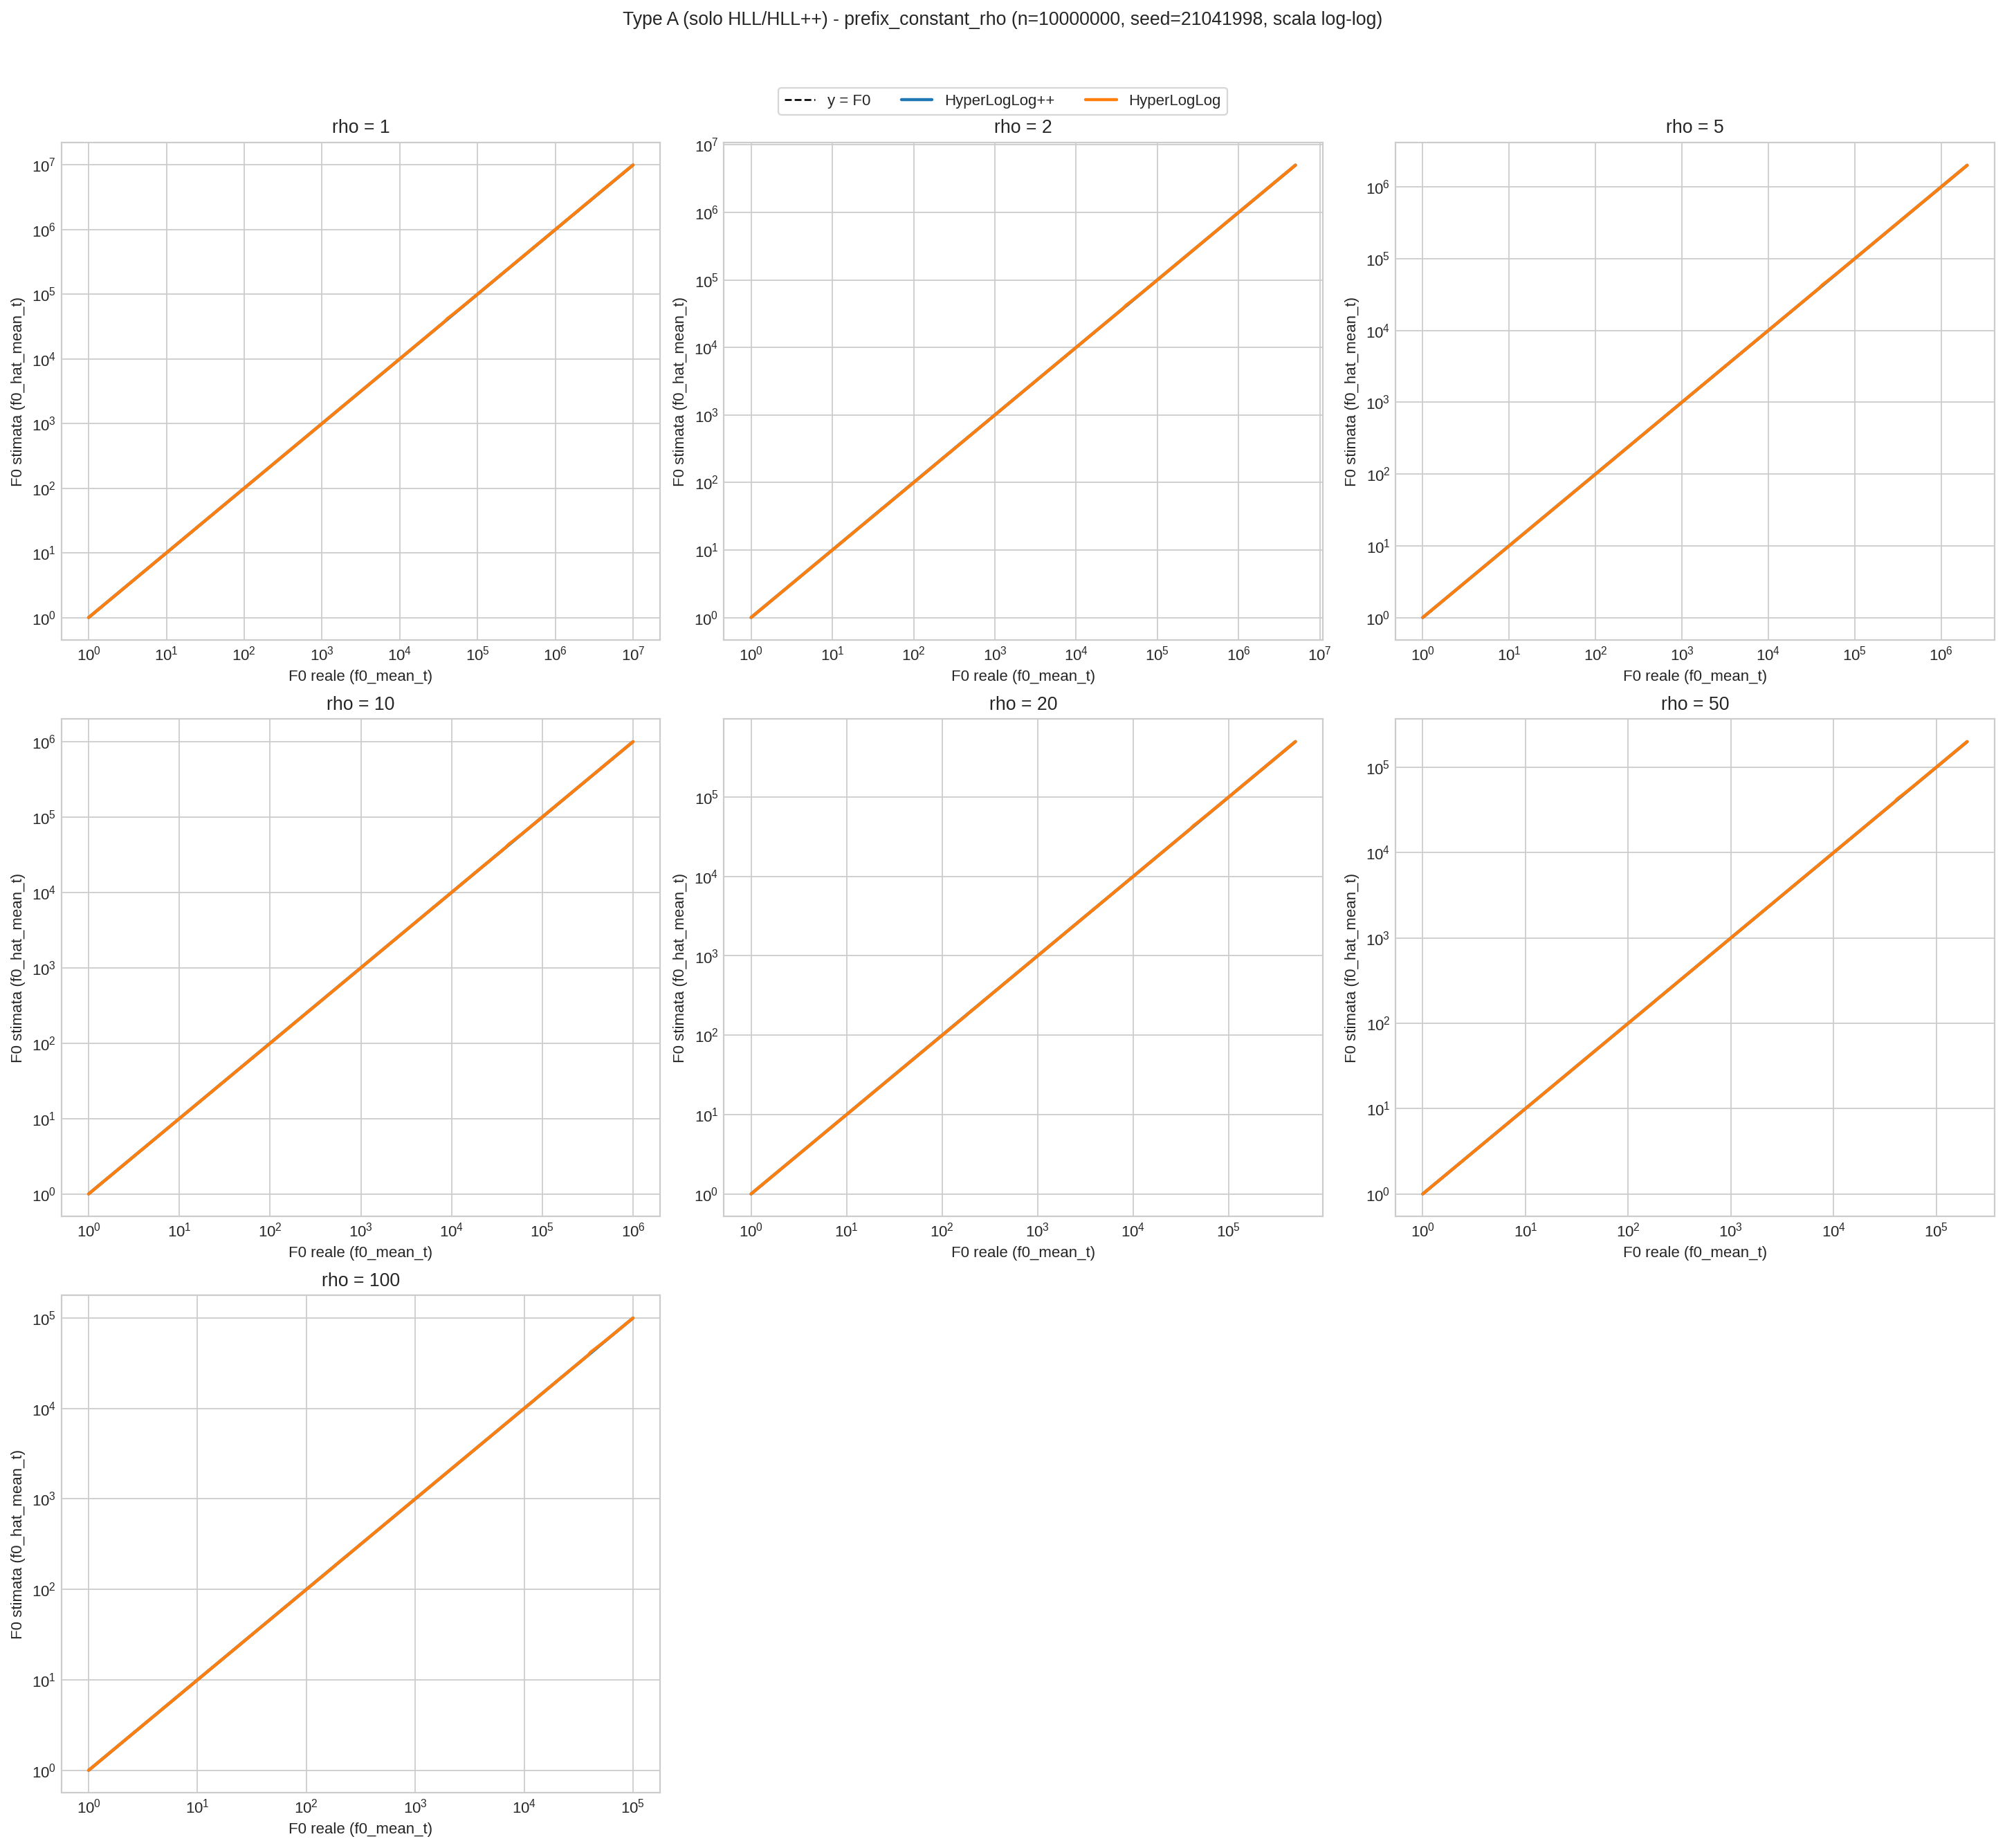
\includegraphics[width=\linewidth]{figures/results/typeA_prefix_constant_rho_hll_hllpp_loglog.png}
        \caption{Scala logaritmica}
        \label{fig:ch5-stream-f0-hll-loglog}
    \end{subfigure}
    \caption{Stima rispetto alla cardinalità reale del prefisso, confronto HyperLogLog e HyperLogLog++}
    \label{fig:ch5-stream-f0-hll}
\end{figure}

\subsubsection{Stima in funzione del rapporto tra elementi processati e distinti}
\label{sec:ch5-streaming-rho}

Questa analisi corrisponde ai grafici precedentemente indicati come
analisi del caso B.
Per ciascun valore obiettivo
\[
F_0^{\ast} \in \{1000,2000,5000,10000,20000,50000,100000\}
\]
si estrae per interpolazione il punto la cui ascissa è il rapporto
\[
\rho_t=\frac{t}{F_0(t)}
\]
e la cui ordinata è la stima corrispondente.

\begin{figure}[p]
    \centering
    \begin{subfigure}[t]{0.49\textwidth}
        \centering
        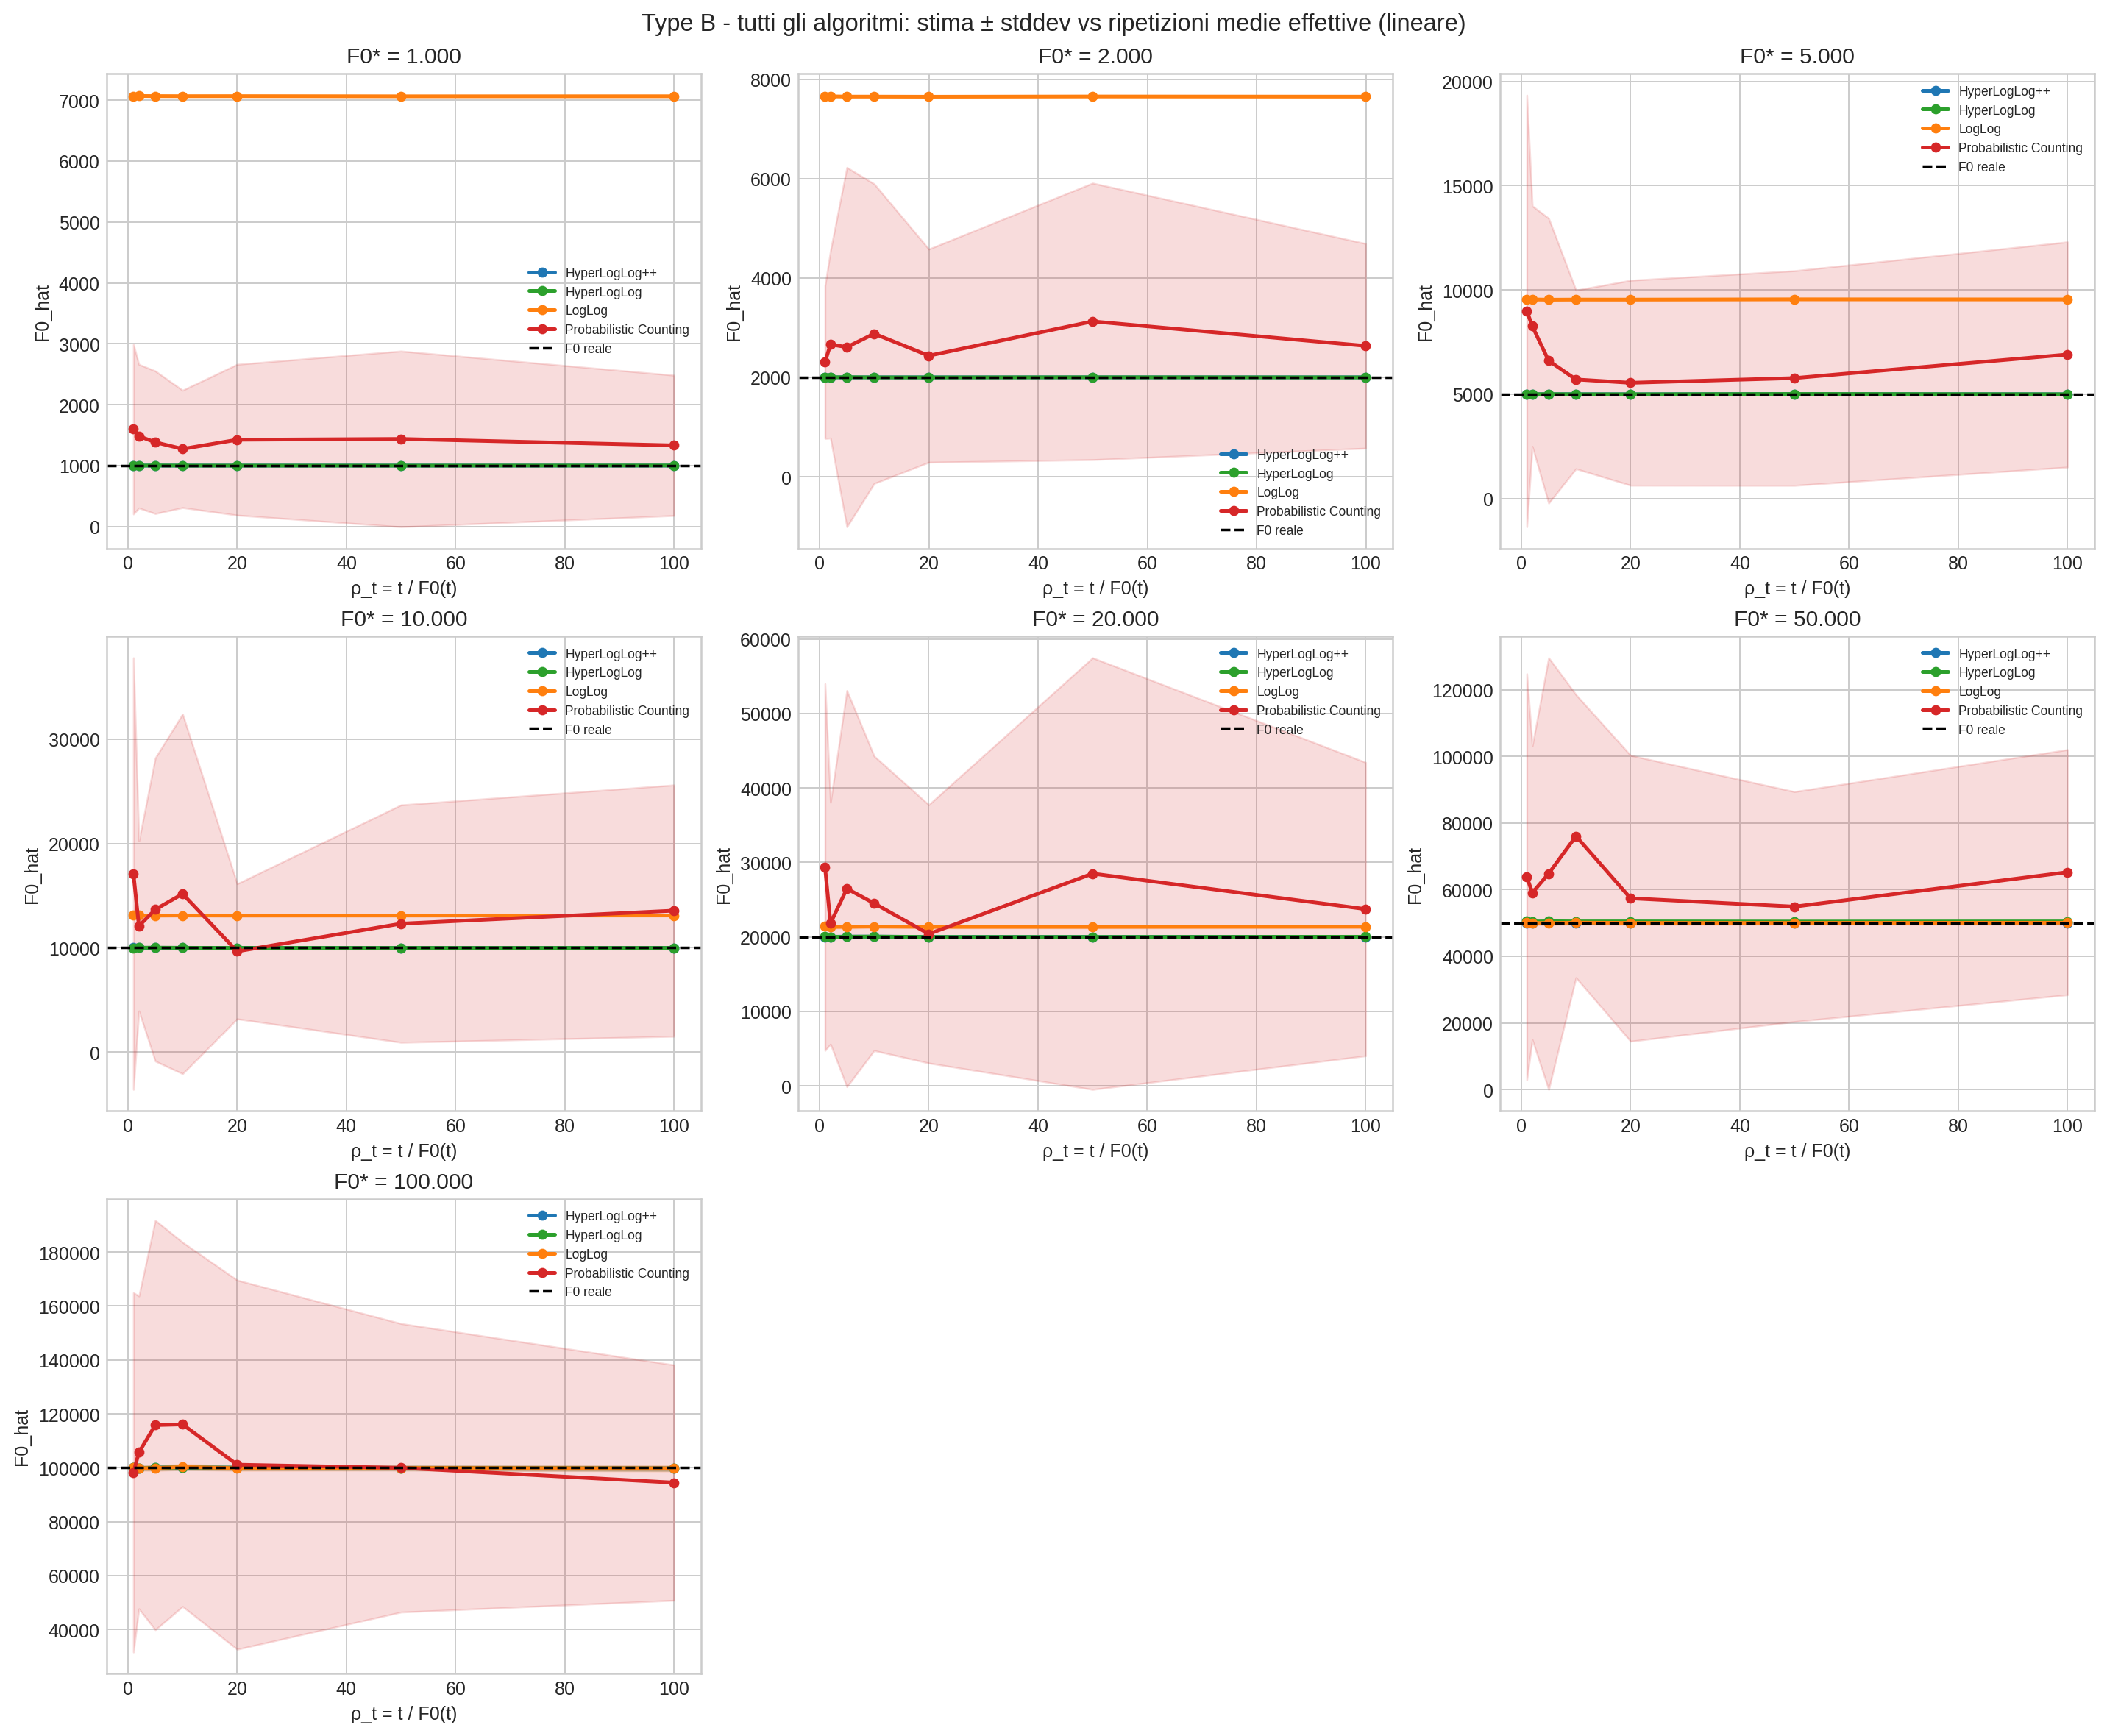
\includegraphics[width=\linewidth]{figures/results/typeB_prefix_constant_rho_all_linear.png}
        \caption{Scala lineare}
        \label{fig:ch5-stream-rho-all-linear}
    \end{subfigure}
    \hfill
    \begin{subfigure}[t]{0.49\textwidth}
        \centering
        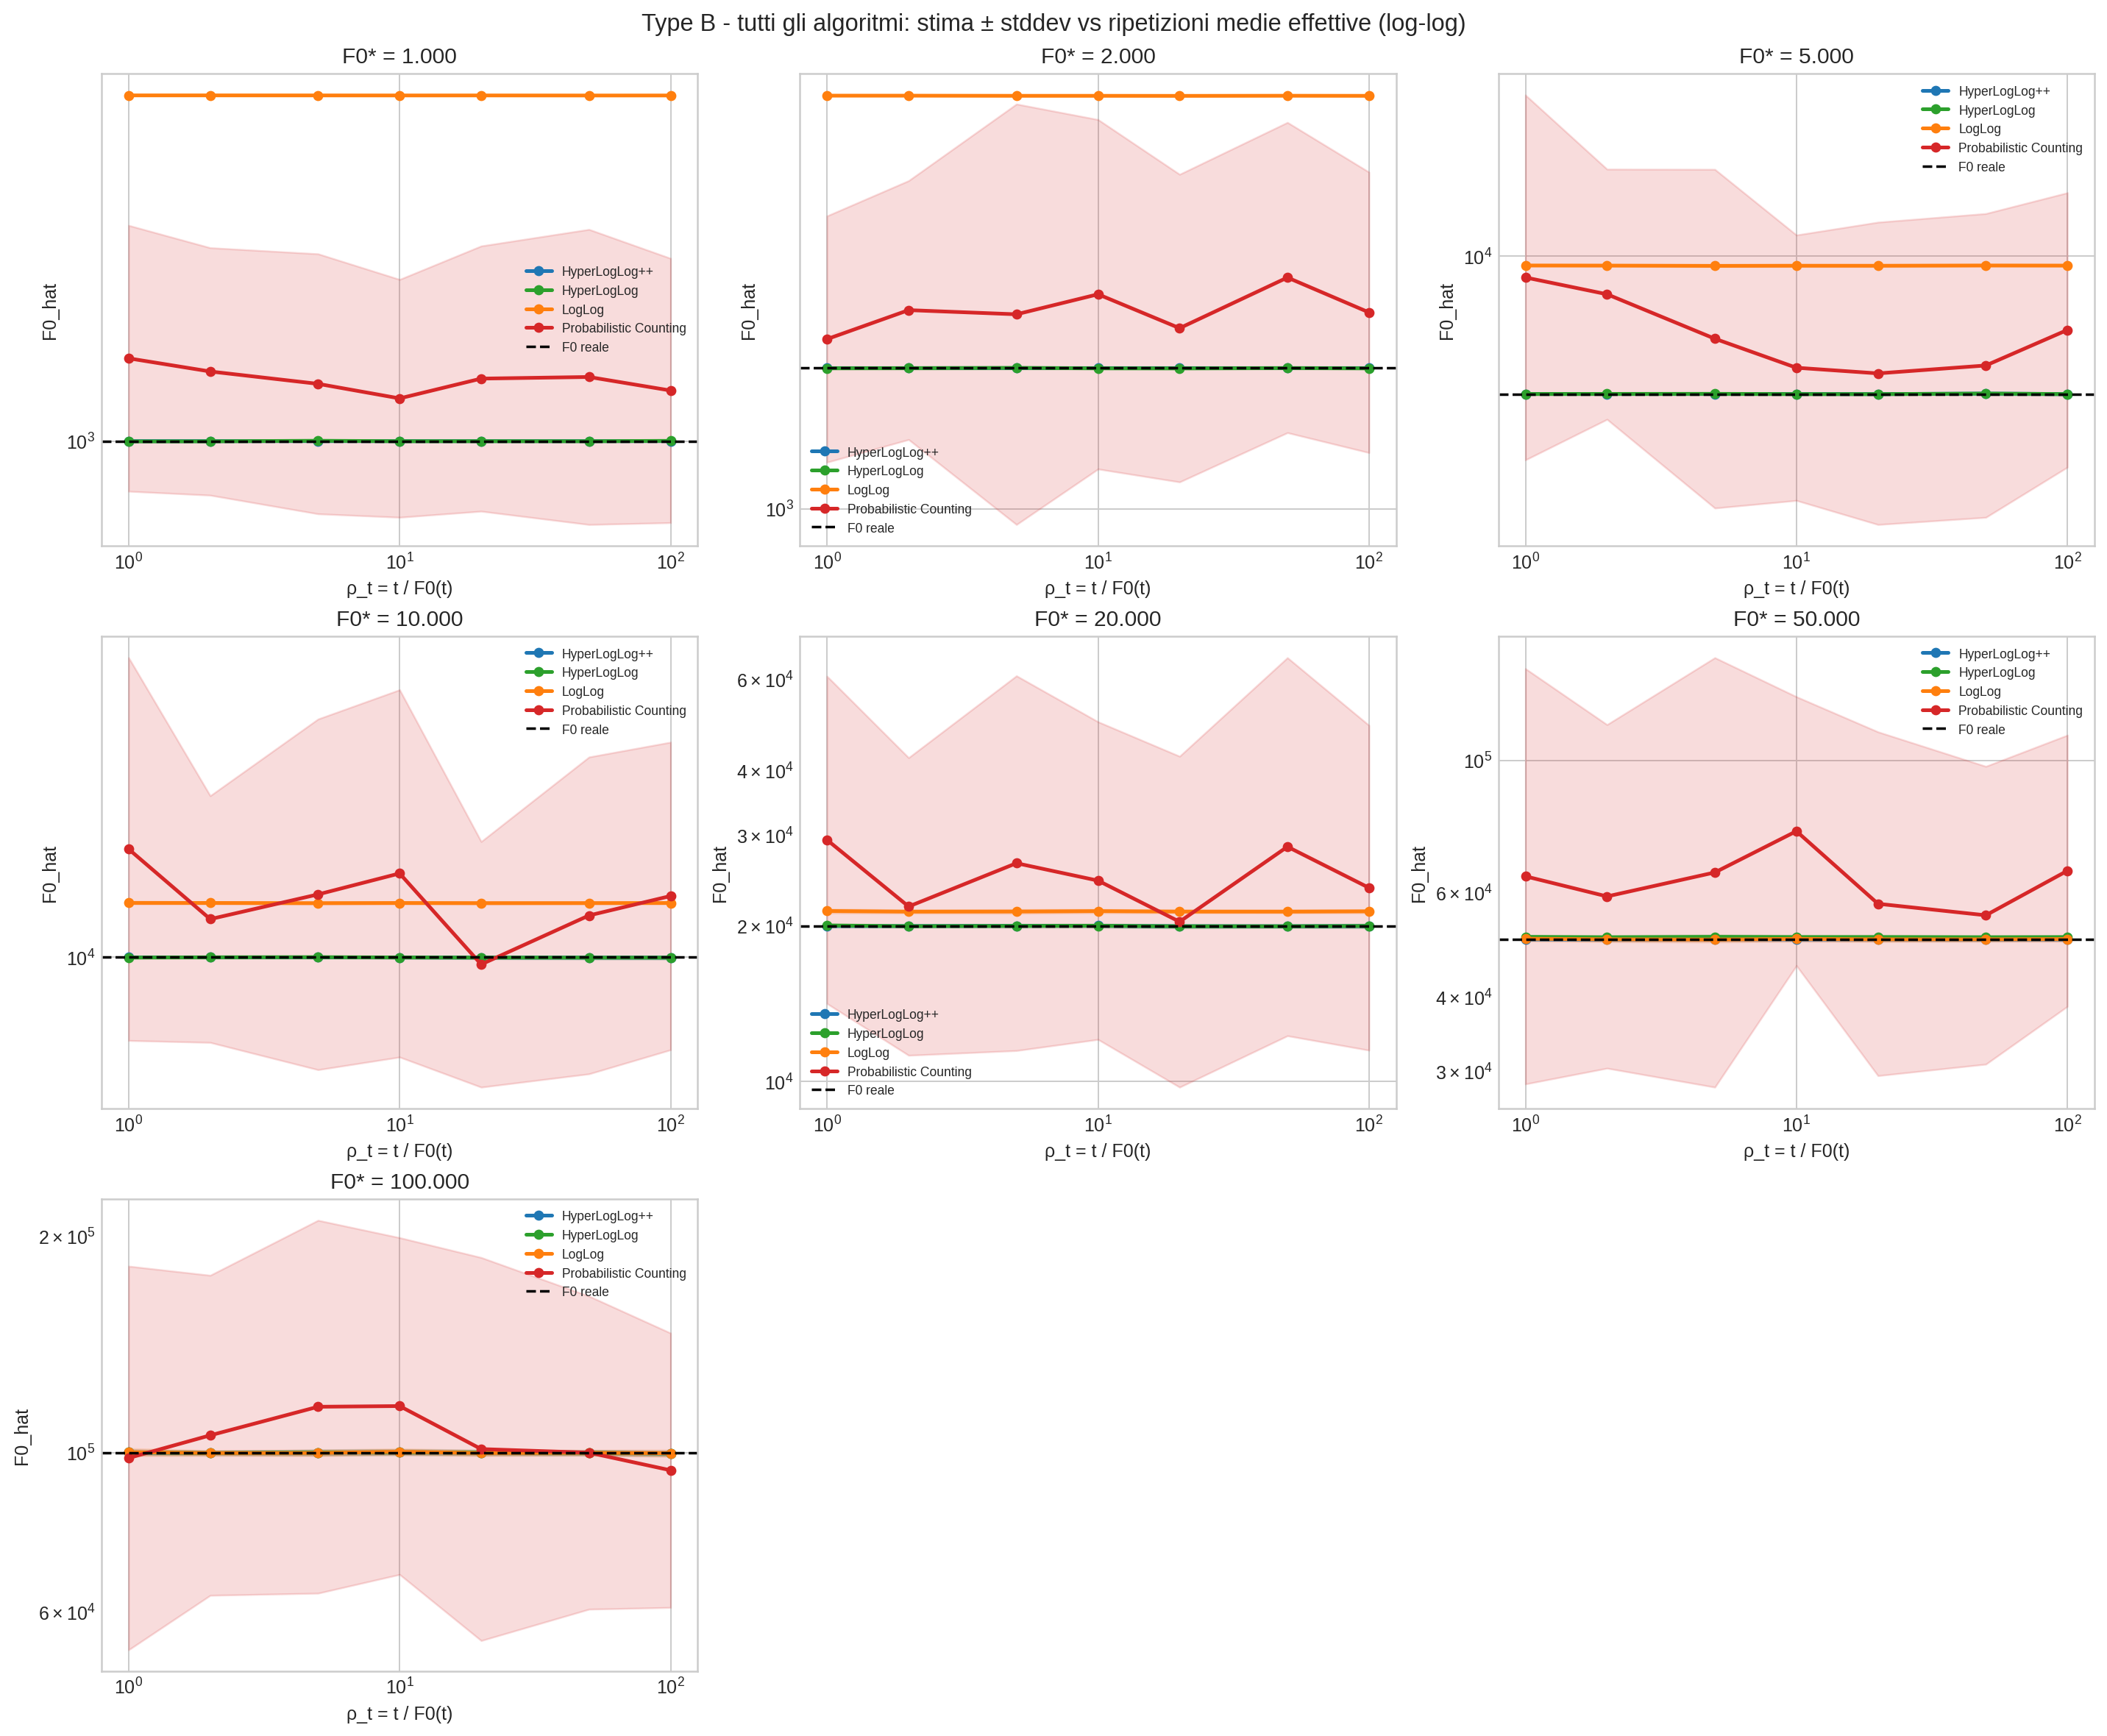
\includegraphics[width=\linewidth]{figures/results/typeB_prefix_constant_rho_all_loglog.png}
        \caption{Scala logaritmica}
        \label{fig:ch5-stream-rho-all-loglog}
    \end{subfigure}
    \caption{Stima rispetto al rapporto tra elementi processati e distinti, tutti gli algoritmi}
    \label{fig:ch5-stream-rho-all}
\end{figure}

\begin{figure}[p]
    \centering
    \begin{subfigure}[t]{0.49\textwidth}
        \centering
        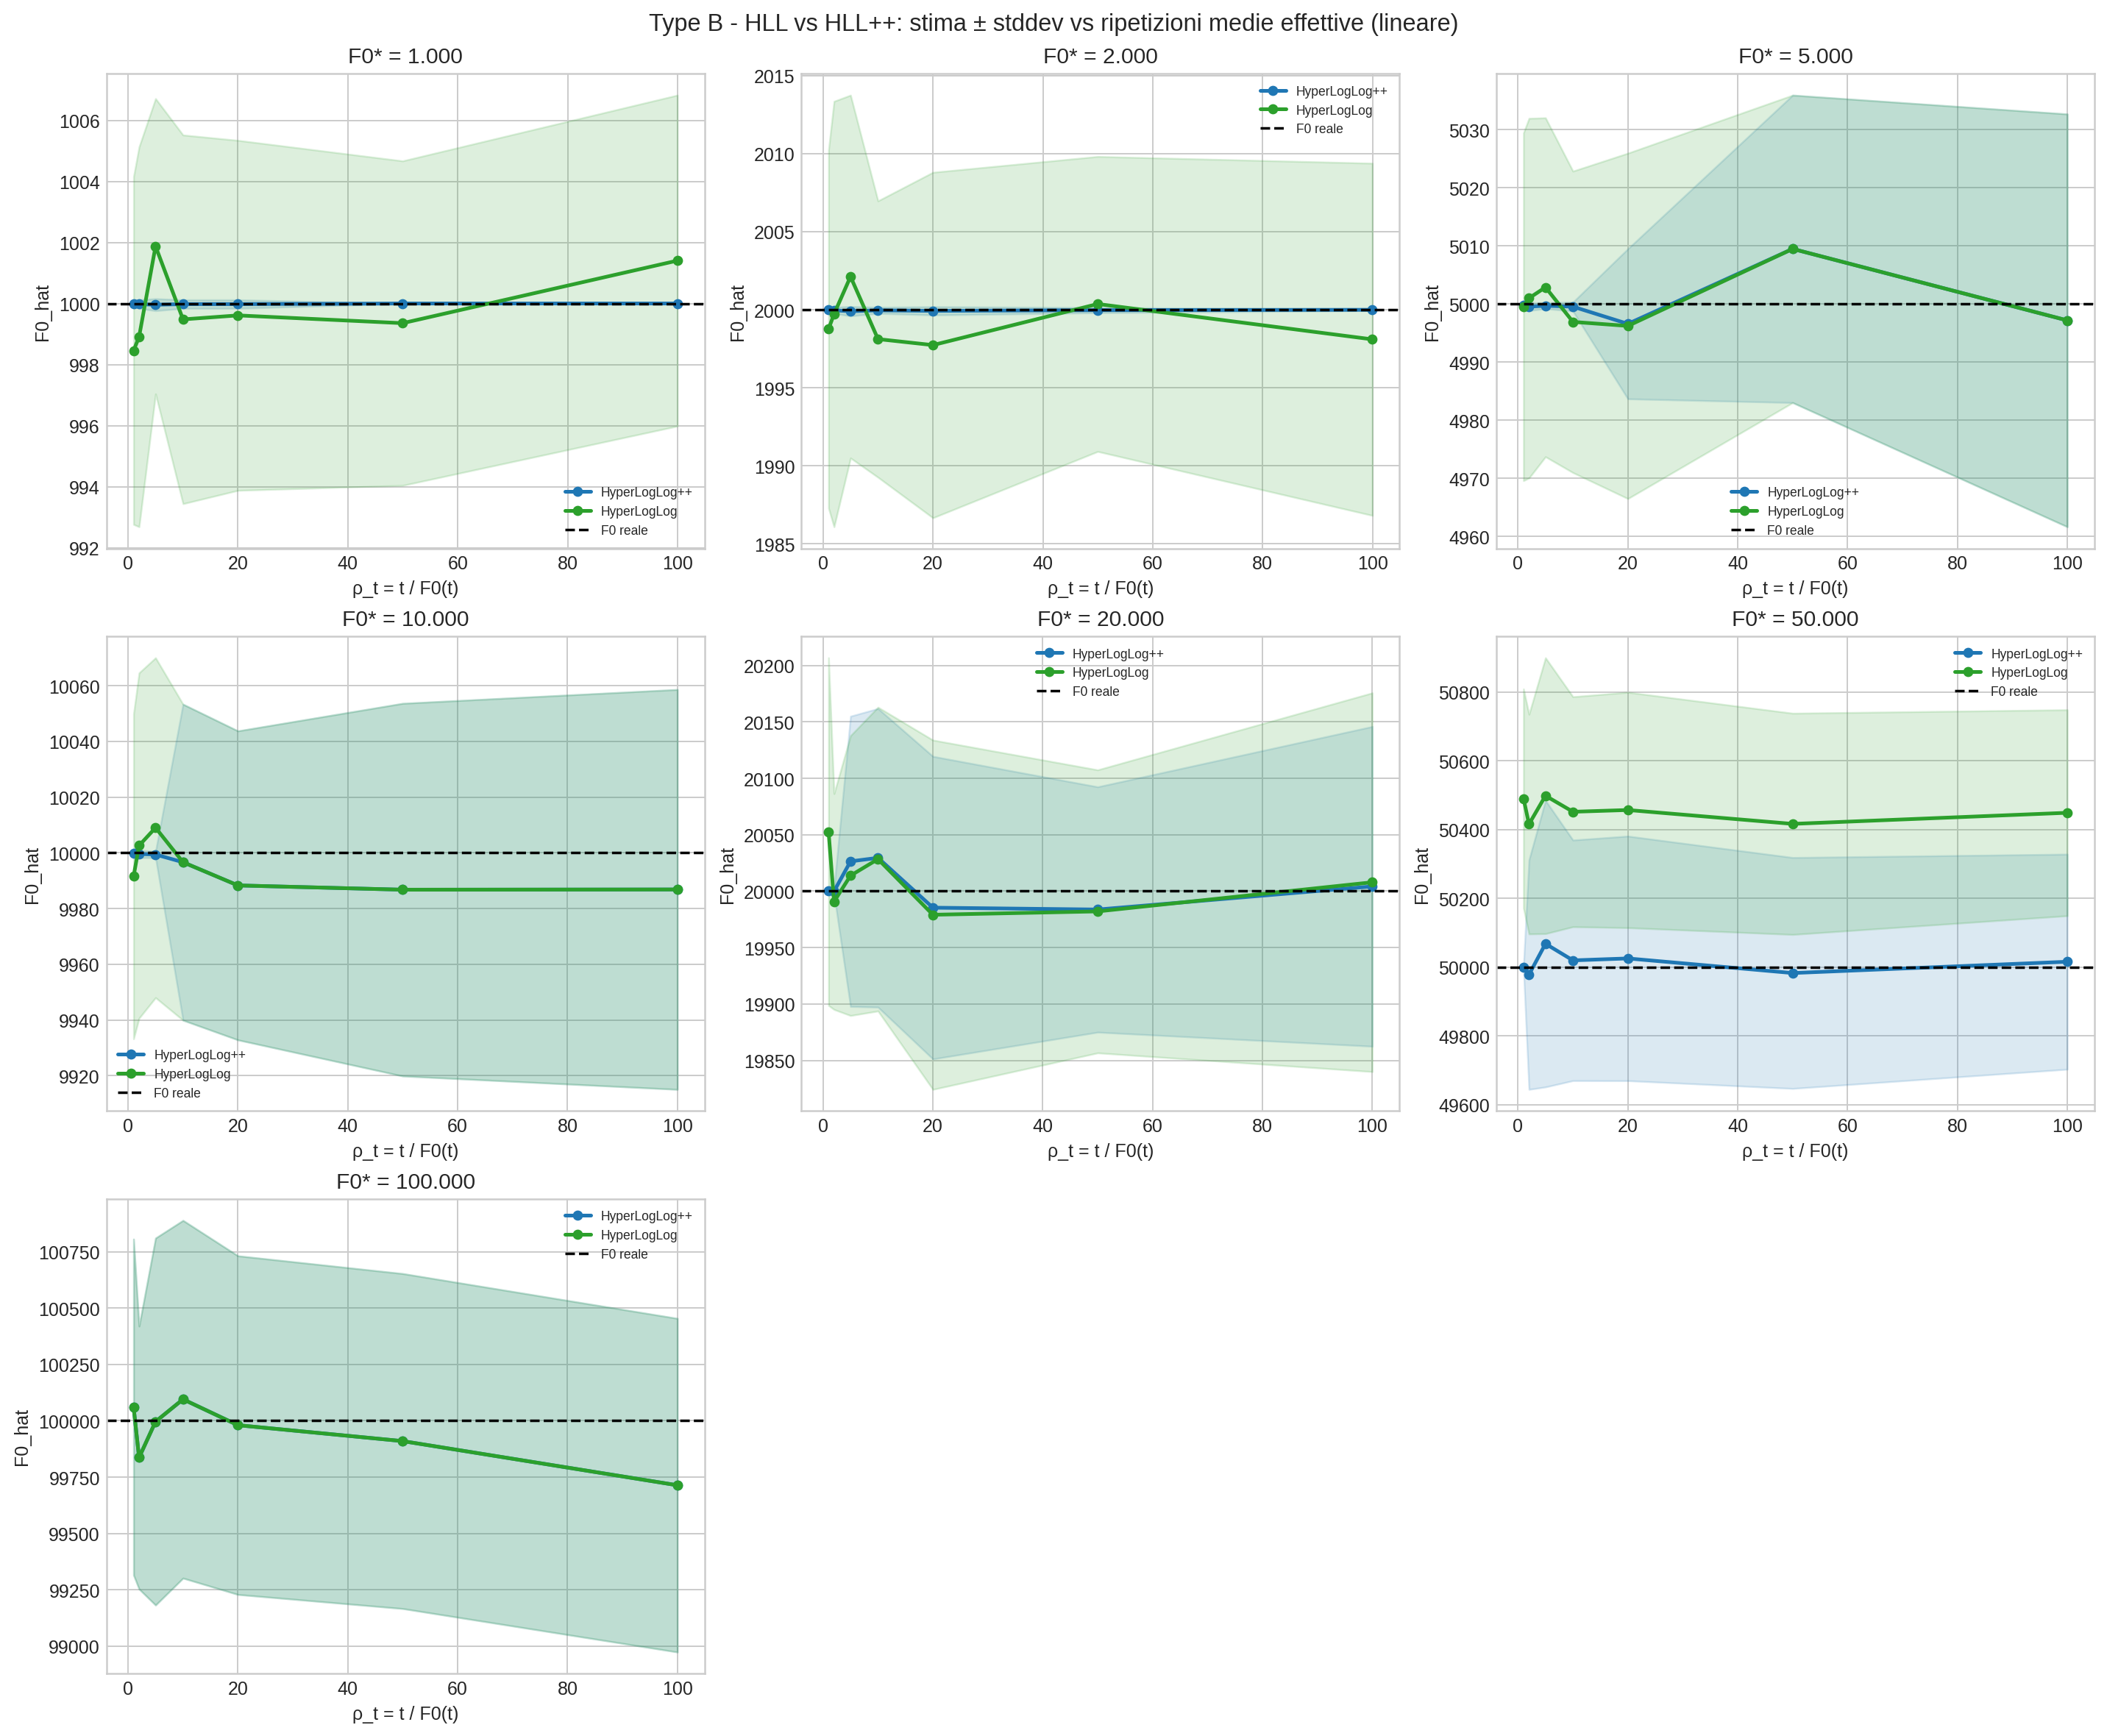
\includegraphics[width=\linewidth]{figures/results/typeB_prefix_constant_rho_hll_hllpp_linear.png}
        \caption{Scala lineare}
        \label{fig:ch5-stream-rho-hll-linear}
    \end{subfigure}
    \hfill
    \begin{subfigure}[t]{0.49\textwidth}
        \centering
        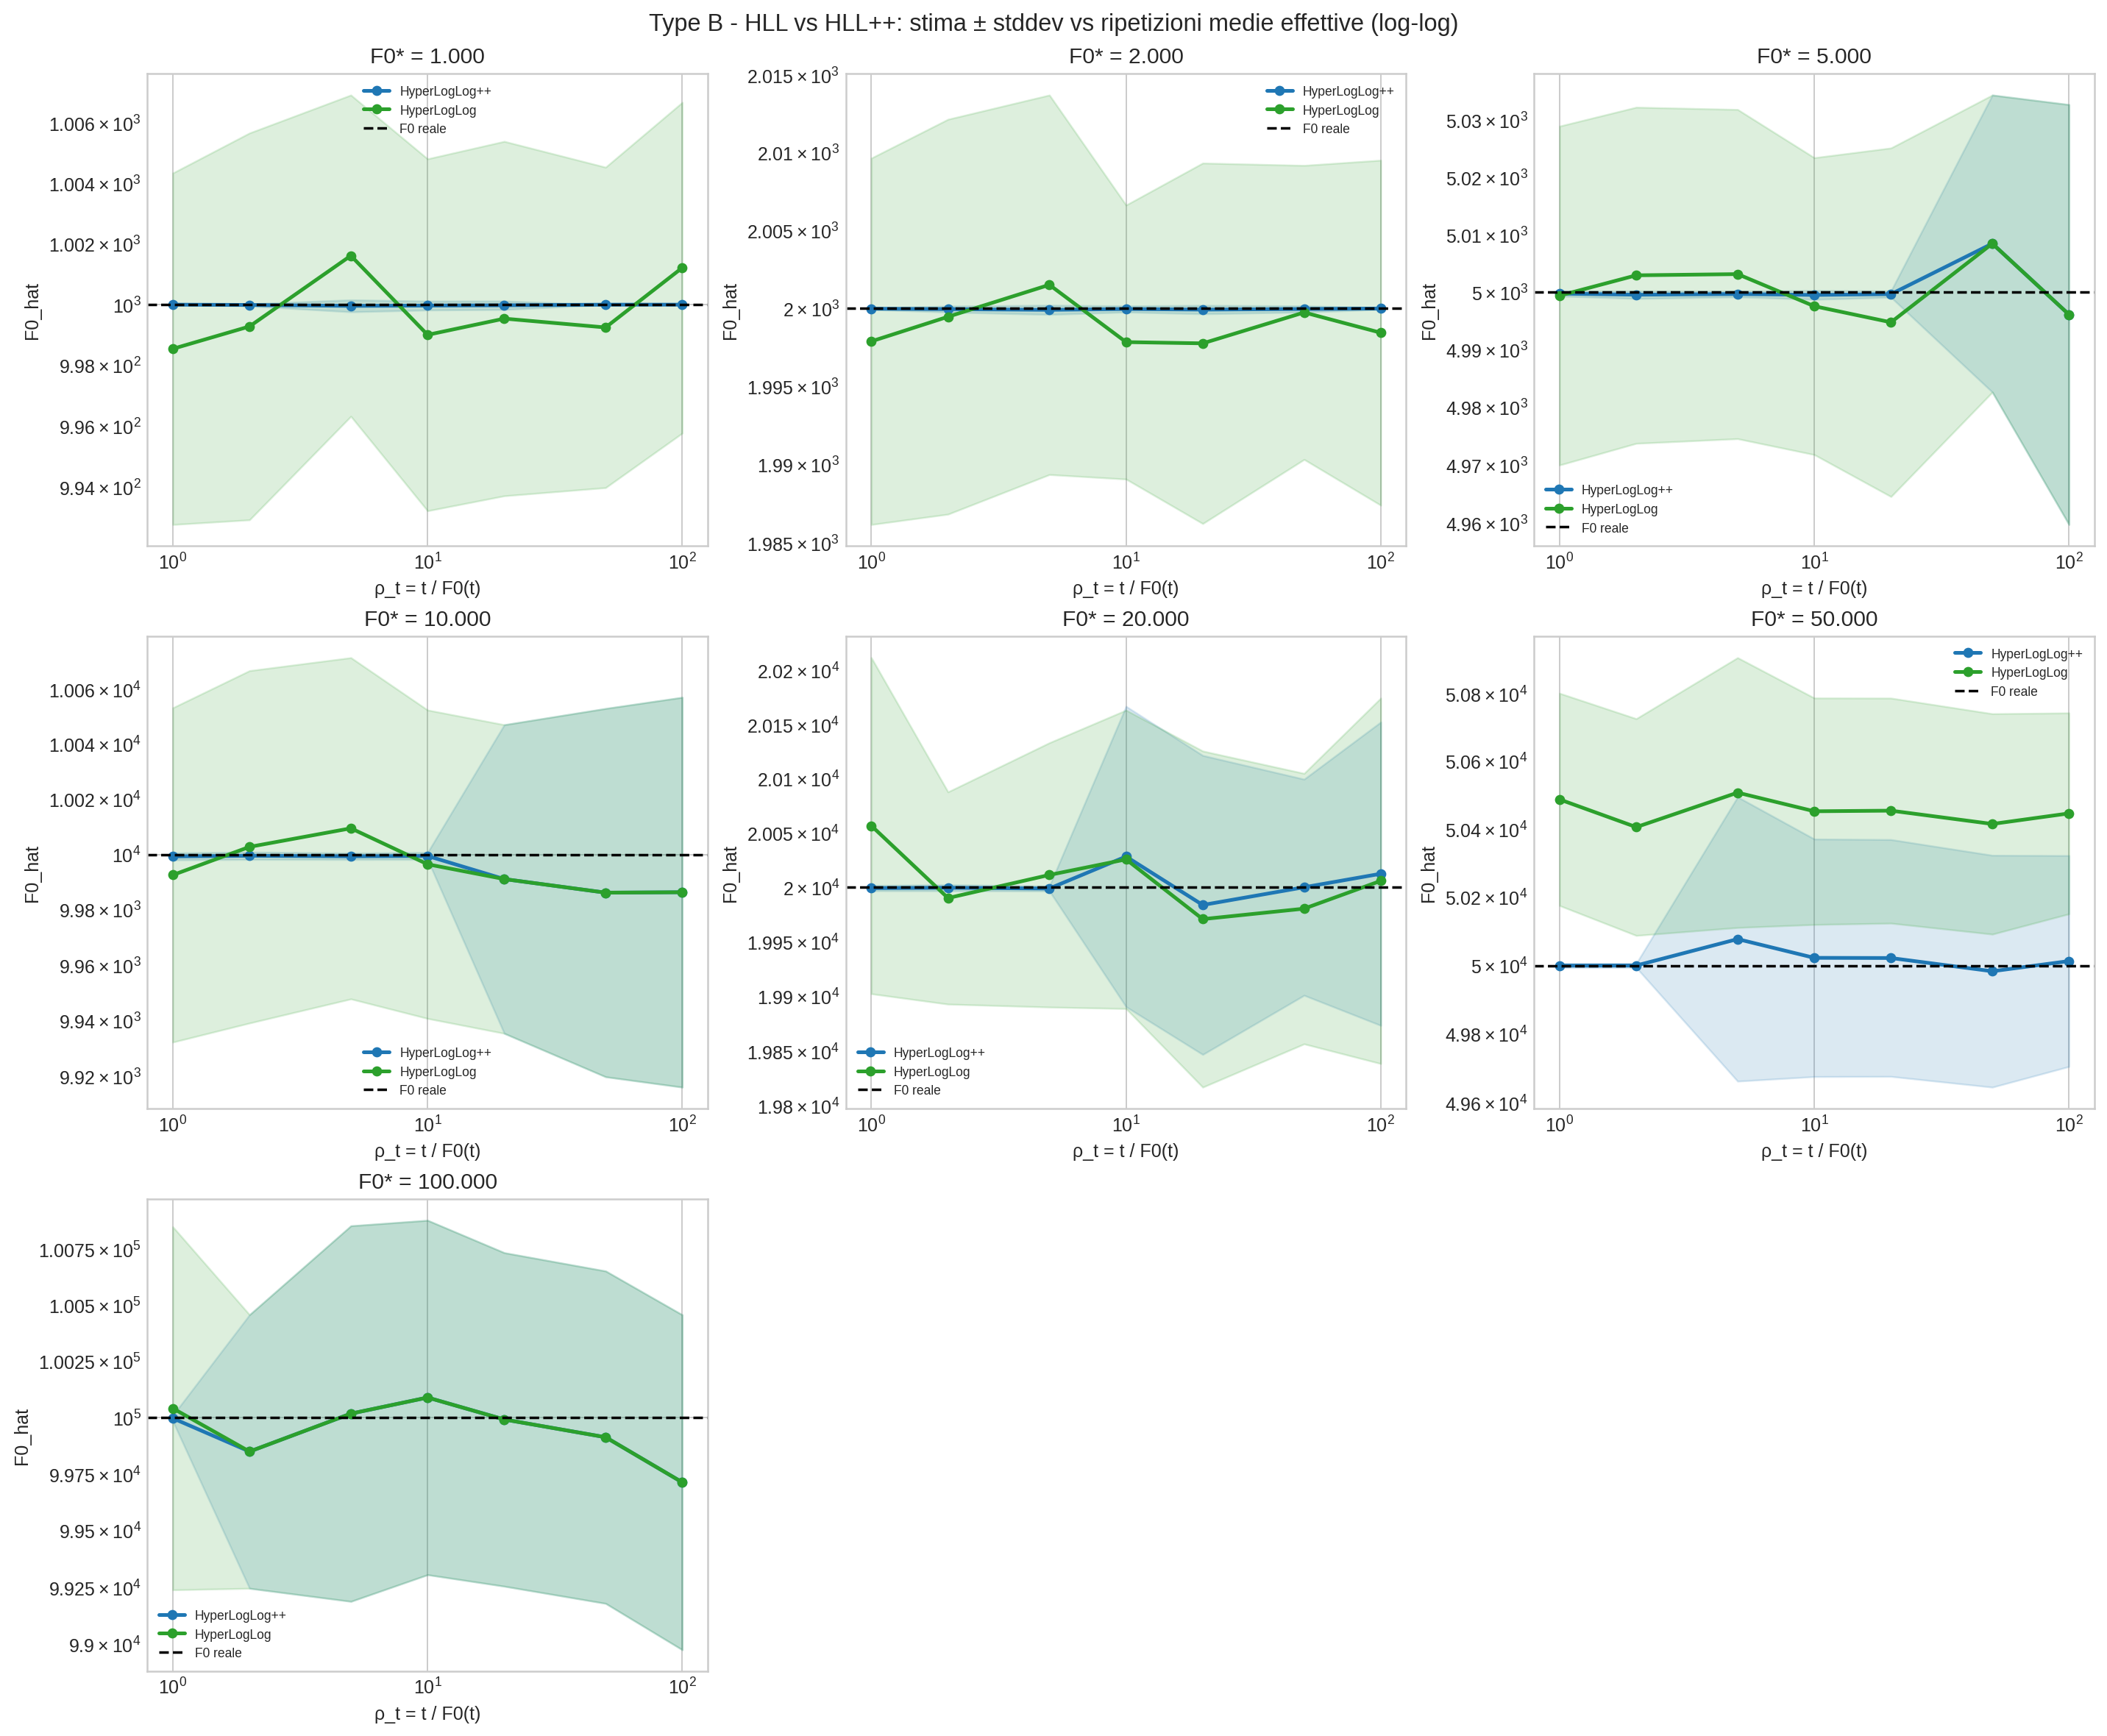
\includegraphics[width=\linewidth]{figures/results/typeB_prefix_constant_rho_hll_hllpp_loglog.png}
        \caption{Scala logaritmica}
        \label{fig:ch5-stream-rho-hll-loglog}
    \end{subfigure}
    \caption{Stima rispetto al rapporto tra elementi processati e distinti, confronto HyperLogLog e HyperLogLog++}
    \label{fig:ch5-stream-rho-hll}
\end{figure}

\subsubsection{Risultati sulla robustezza e sul bias}
Le osservazioni principali emerse dai riassunti ai punti finali osservati sono:
\begin{itemize}
    \item nella vista rispetto alla cardinalità reale del prefisso,
    HyperLogLog e HyperLogLog++ risultano quasi sovrapposti, con errore
    relativo medio ai punti finali di circa \(0.00618\);
    \item nella stessa vista, LogLog segue con errore medio di circa
    \(0.00708\), mentre Probabilistic Counting è nettamente più instabile con
    errore medio di circa \(0.770\);
    \item nella vista rispetto al rapporto tra elementi processati e distinti,
    HyperLogLog++ è l'algoritmo più accurato con errore medio di circa
    \(3.95\cdot 10^{-4}\);
    \item HyperLogLog segue con errore medio di circa \(2.08\cdot 10^{-3}\);
    \item nella stessa vista, Probabilistic Counting ha errore medio di circa
    \(0.346\);
    \item nella seconda vista, l'errore medio più alto è osservato per LogLog,
    con valore di circa \(1.455\).
\end{itemize}

Le Figure~\ref{fig:ch5-stream-f0-hll} e \ref{fig:ch5-stream-rho-hll}
confermano che HyperLogLog++ mantiene il comportamento più stabile nelle due
viste complementari del problema.

\begin{figure}[htbp]
    \centering
    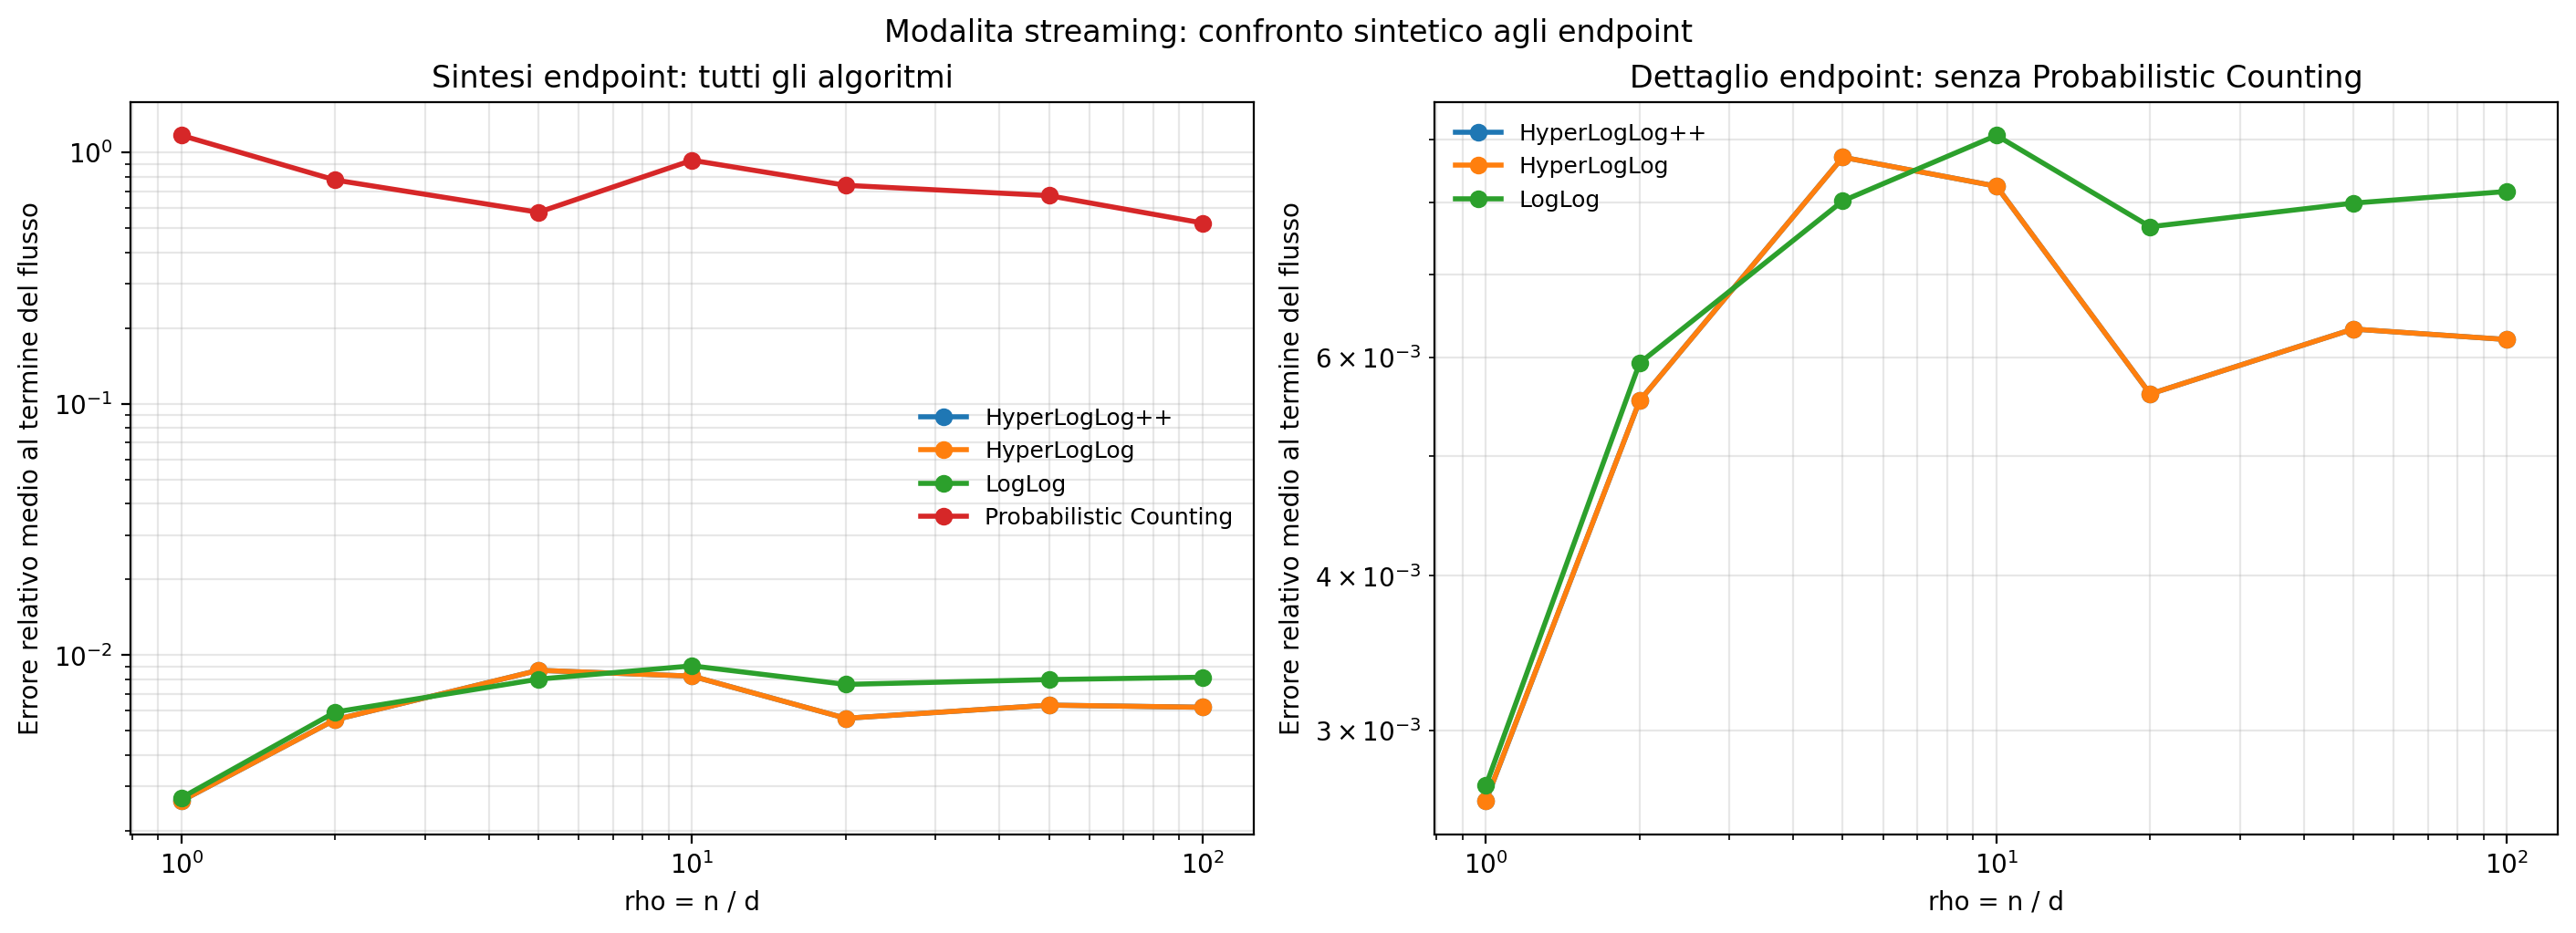
\includegraphics[width=0.98\textwidth]{figures/results/streaming_endpoint_mre_summary.png}
    \caption{Errore relativo medio alla fine della stream. Il pannello sinistro confronta tutti gli algoritmi, mentre quello destro isola HyperLogLog++, HyperLogLog e LogLog}
    \label{fig:ch5-stream-endpoint-summary}
\end{figure}

La Figura~\ref{fig:ch5-stream-endpoint-summary} riassume in forma compatta la
stessa evidenza: Probabilistic Counting resta nettamente separato dagli altri
algoritmi, mentre HyperLogLog++ mantiene il comportamento più regolare e
accurato nel confronto complessivo. Questo risultato è coerente con la
letteratura su HLL++, in cui la riduzione empirica del bias e la gestione
separata dei regimi di cardinalità piccola e intermedia spiegano il vantaggio
rispetto a HLL classico \cite{Heule_Nunkesser_Hall_2013}. Più in generale, i
grafici osservati restano compatibili con la linea evolutiva che porta da
LogLog a HyperLogLog e poi a HyperLogLog++, cioè a una progressiva riduzione
della varianza e del bias pratico
\cite{Durand_Flajolet_2003,Flajolet_Fusy_Gandouet_Meunier_2007,Heule_Nunkesser_Hall_2013}.

\subsection{Analisi sulla variazione dei parametro degli algoritmi}
Per analizzare il comportamento degli algoritmi al variare della precisione, 
\`e necessario isolare l'effetto del parametro.

Di conseguenza, \`e stato fatto un secondo insieme di esperimenti in cui 
sono stati fissati lo stesso insieme di
dati, lo stesso seed e la stessa funzione di hash, variando solo il parametro
interno di ciascun
algoritmo.

L'impostazione scelta per questo esperimento comprende:
\begin{itemize}
    \item l'utilizzo della funzione di hash \texttt{splitmix64}
    \item un seed fissato a \(21041998\)
    \item tre valori rappresentativi per \(\rho \in \{1,10,100\}\)
    \item HyperLogLog++ con \(k \in \{8,10,12,14,16,18\}\)
    \item HyperLogLog e LogLog con \(k \in \{4,6,8,10,12,14,16\}\) e \(L=32\)
    \item Probabilistic Counting con \(L \in \{4,8,12,16,20,24,28,31\}\)
\end{itemize}

Per analizzare il comportamento degli algoritmi al variare della precisione, 
sono stati realizzati due tipi di grafici.

Il primo, tramite una heatmap, riassume l'errore relativo medio alla fine 
del flusso di streaming per ogni coppia di
valori tra \(\rho\) e il parametro dell'algoritmo.

Il secondo sia in scala lineare che in scala logaritmica, fissando $\rho$, mette a confronto la cardinalità reale del flusso 
e la stima, dove ogni retta \`e una diversa precisione dell'algoritmo.
\begin{figure}[htbp]
    \centering
    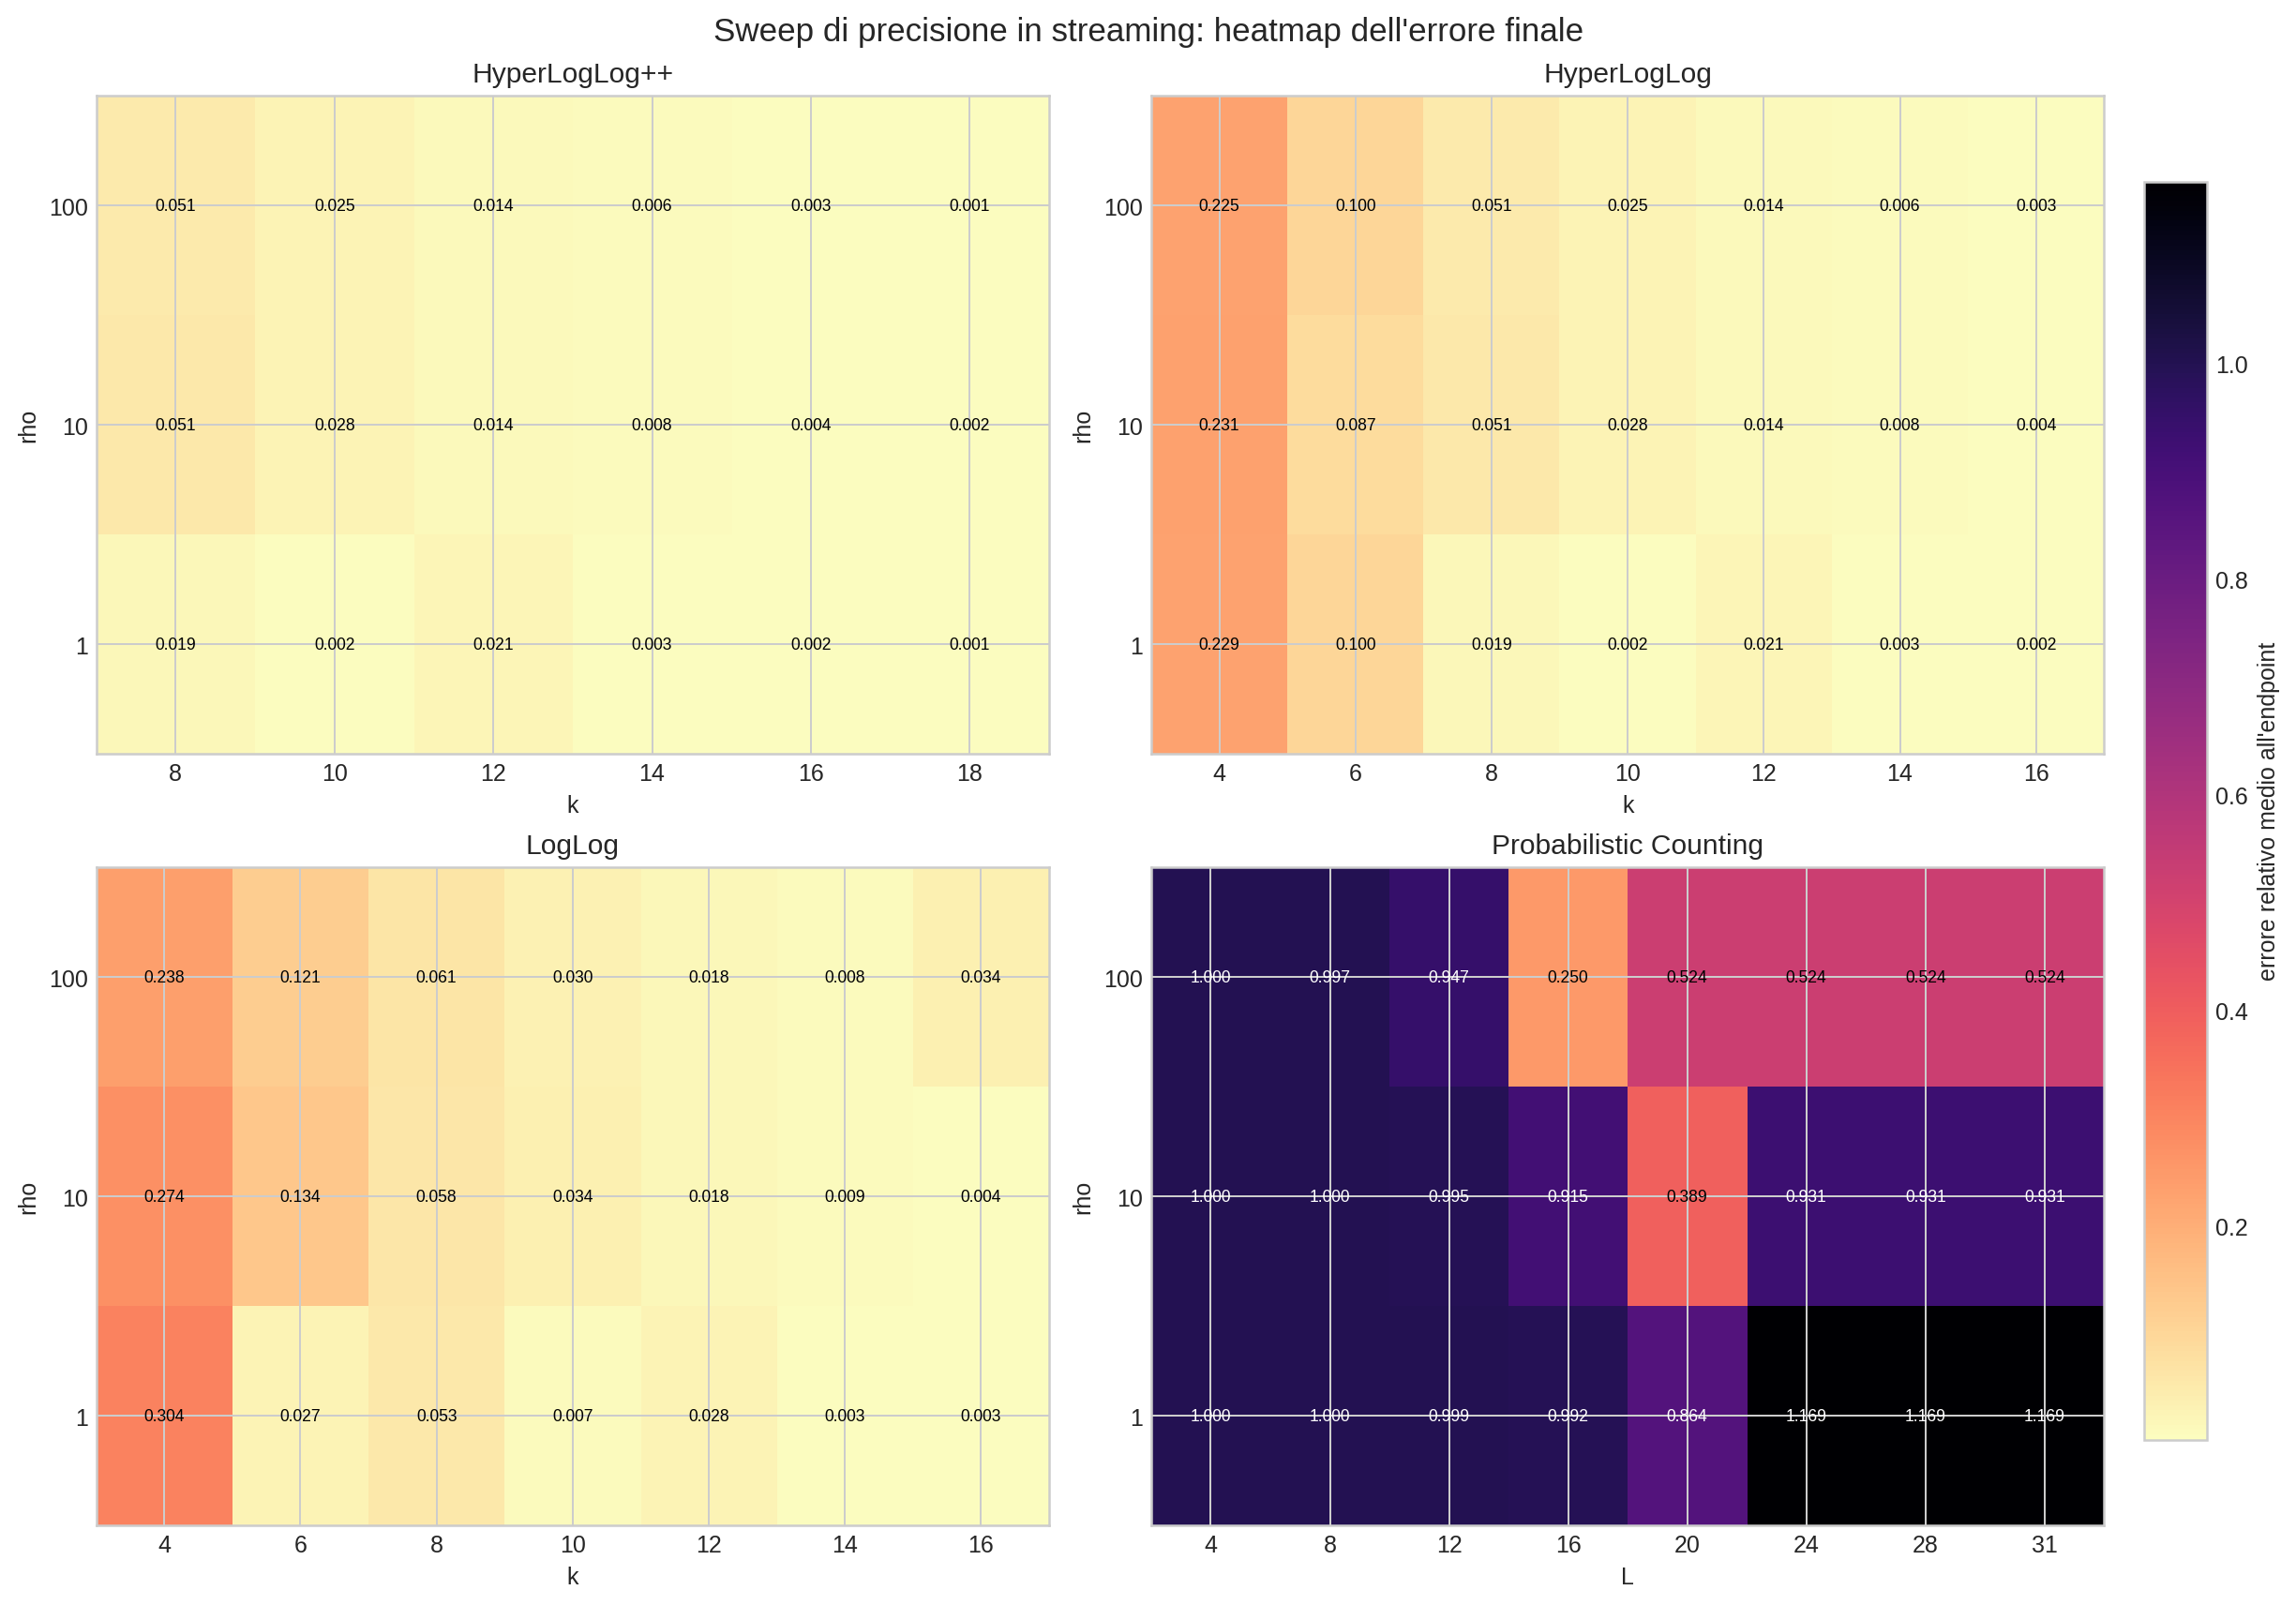
\includegraphics[width=0.98\textwidth]{figures/results/streaming_precision_sweep_endpoint_heatmaps.png}
    \caption{Errore relativo medio alla fine della stream al variare del parametro di precisione e di \(\rho\), per ciascun algoritmo}
    \label{fig:ch5-stream-precision-heatmaps}
\end{figure}

\begin{figure}[p]
    \centering
    \begin{subfigure}[t]{0.49\textwidth}
        \centering
        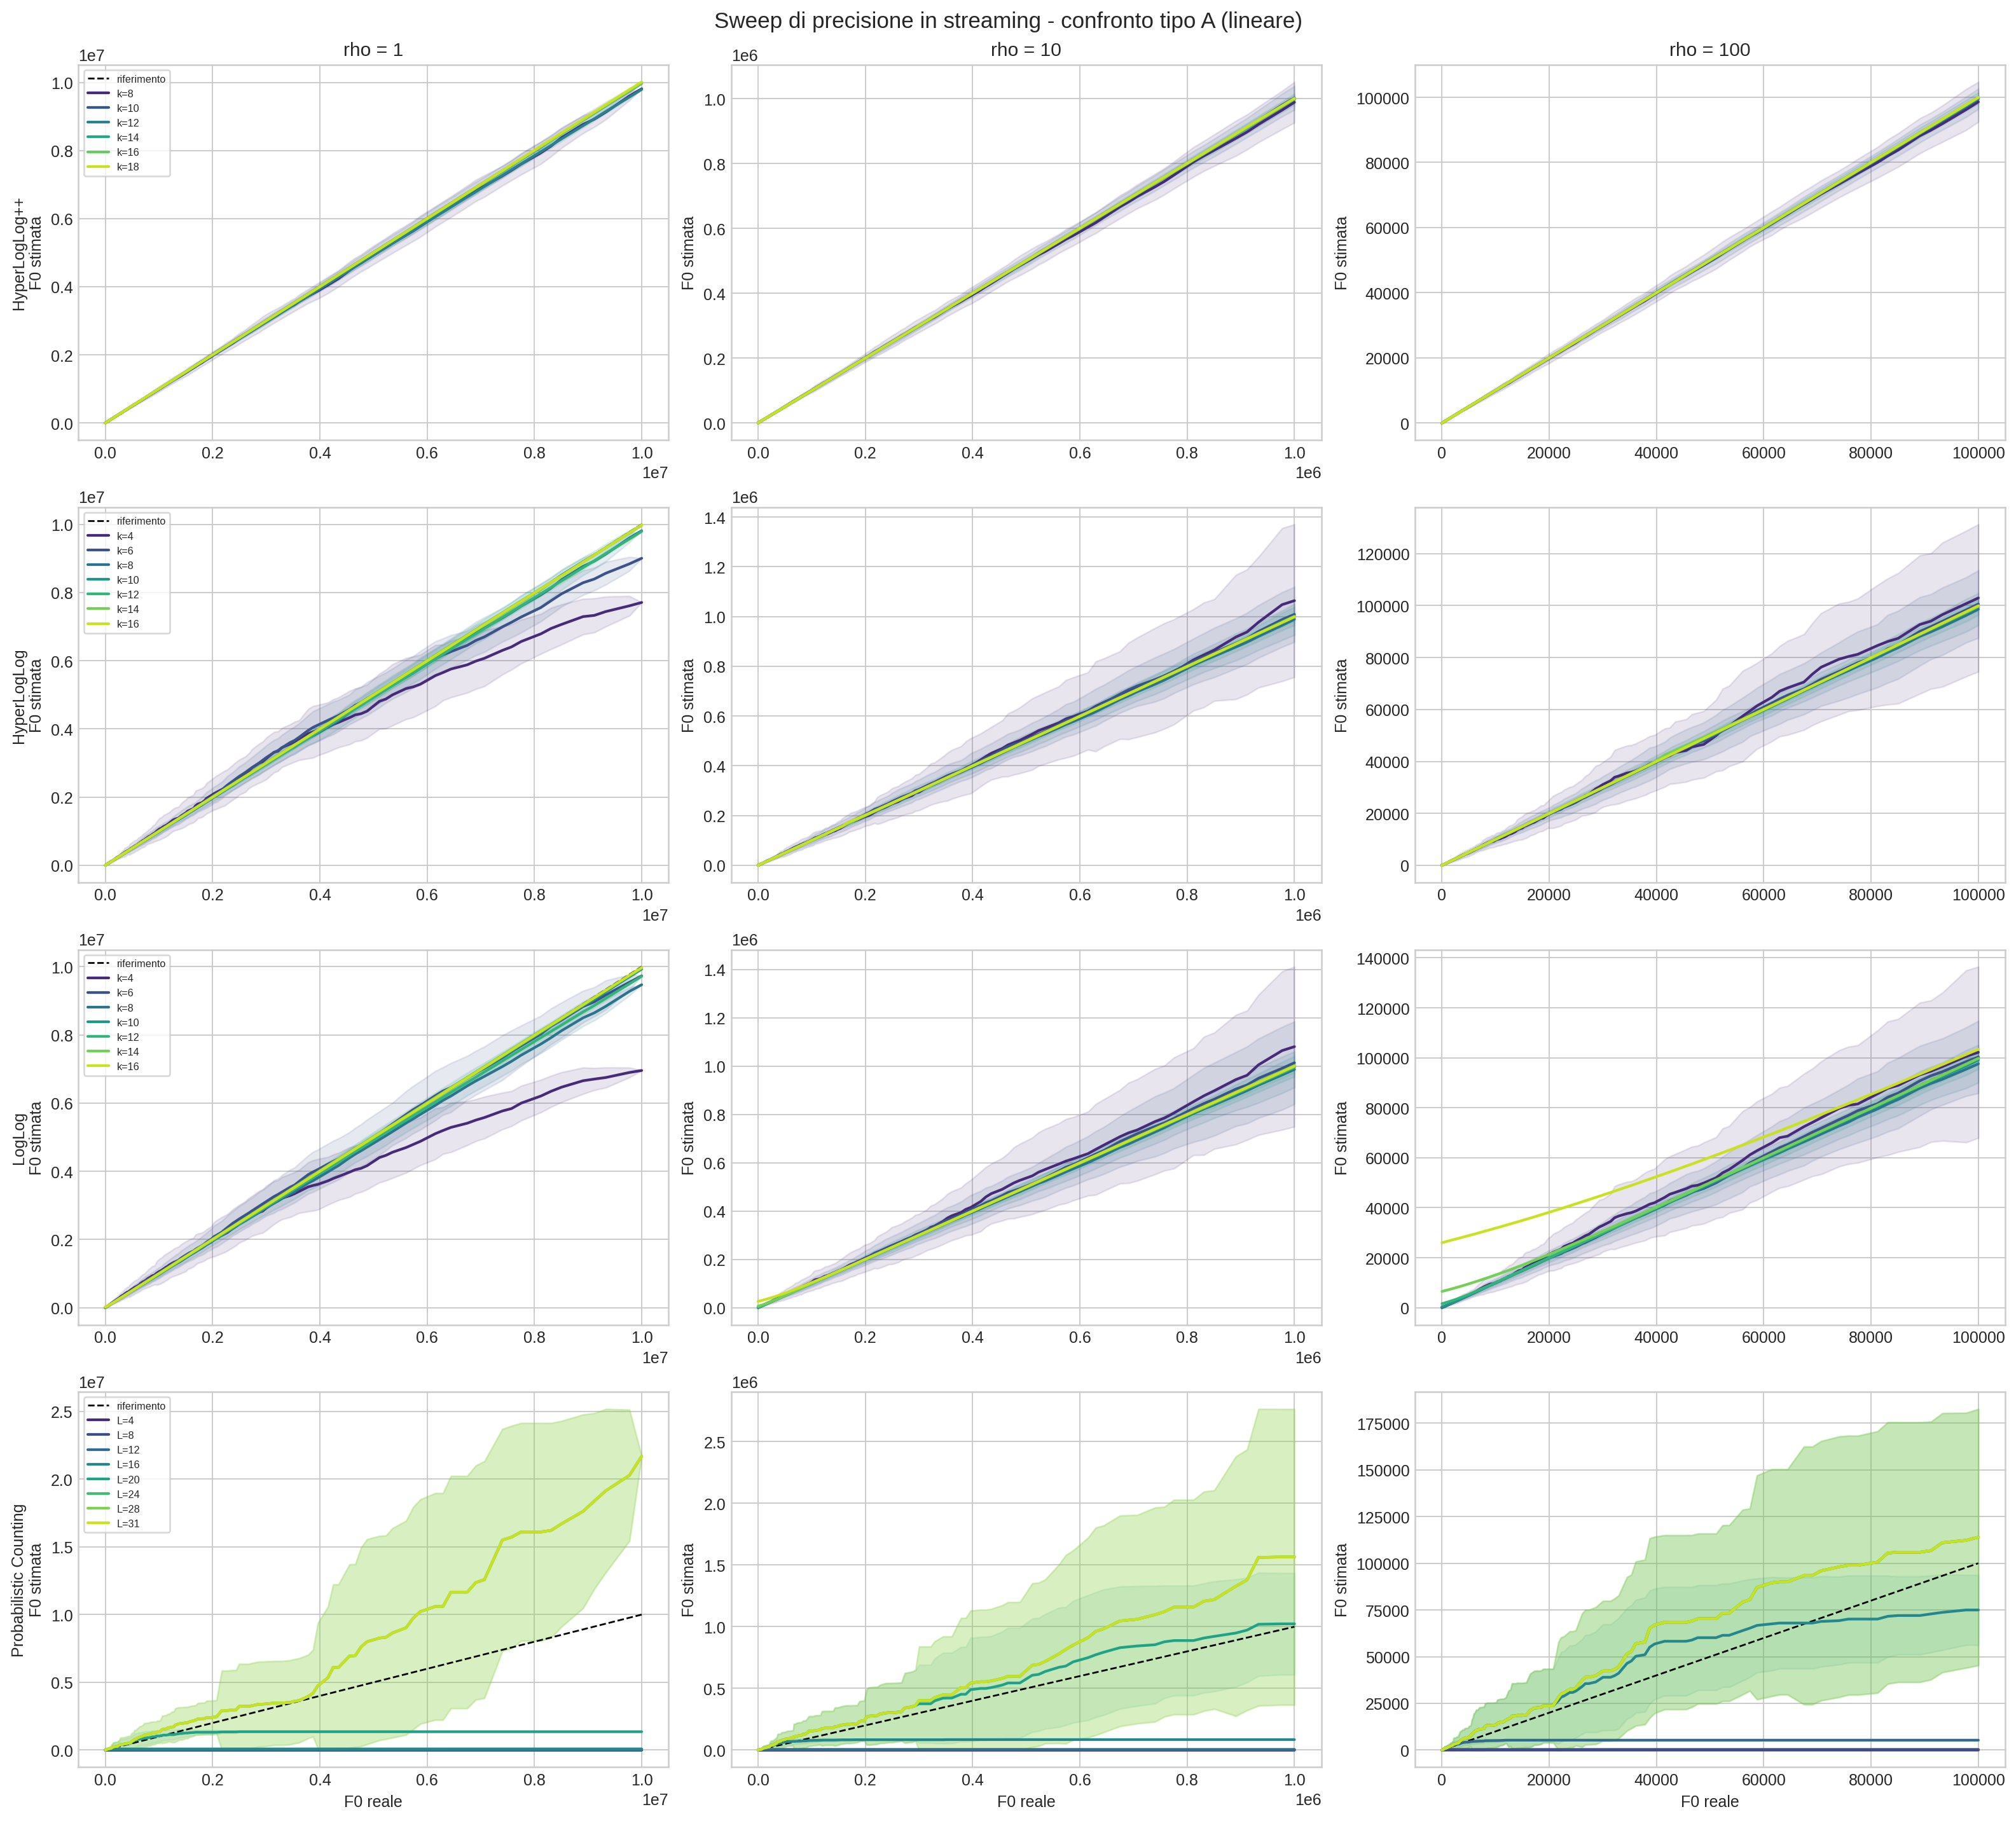
\includegraphics[height=0.33\textheight,keepaspectratio]{figures/results/streaming_precision_sweep_typeA_grid_linear.png}
        \caption{Scala lineare}
        \label{fig:ch5-stream-precision-typea-linear}
    \end{subfigure}
    \hfill
    \begin{subfigure}[t]{0.49\textwidth}
        \centering
        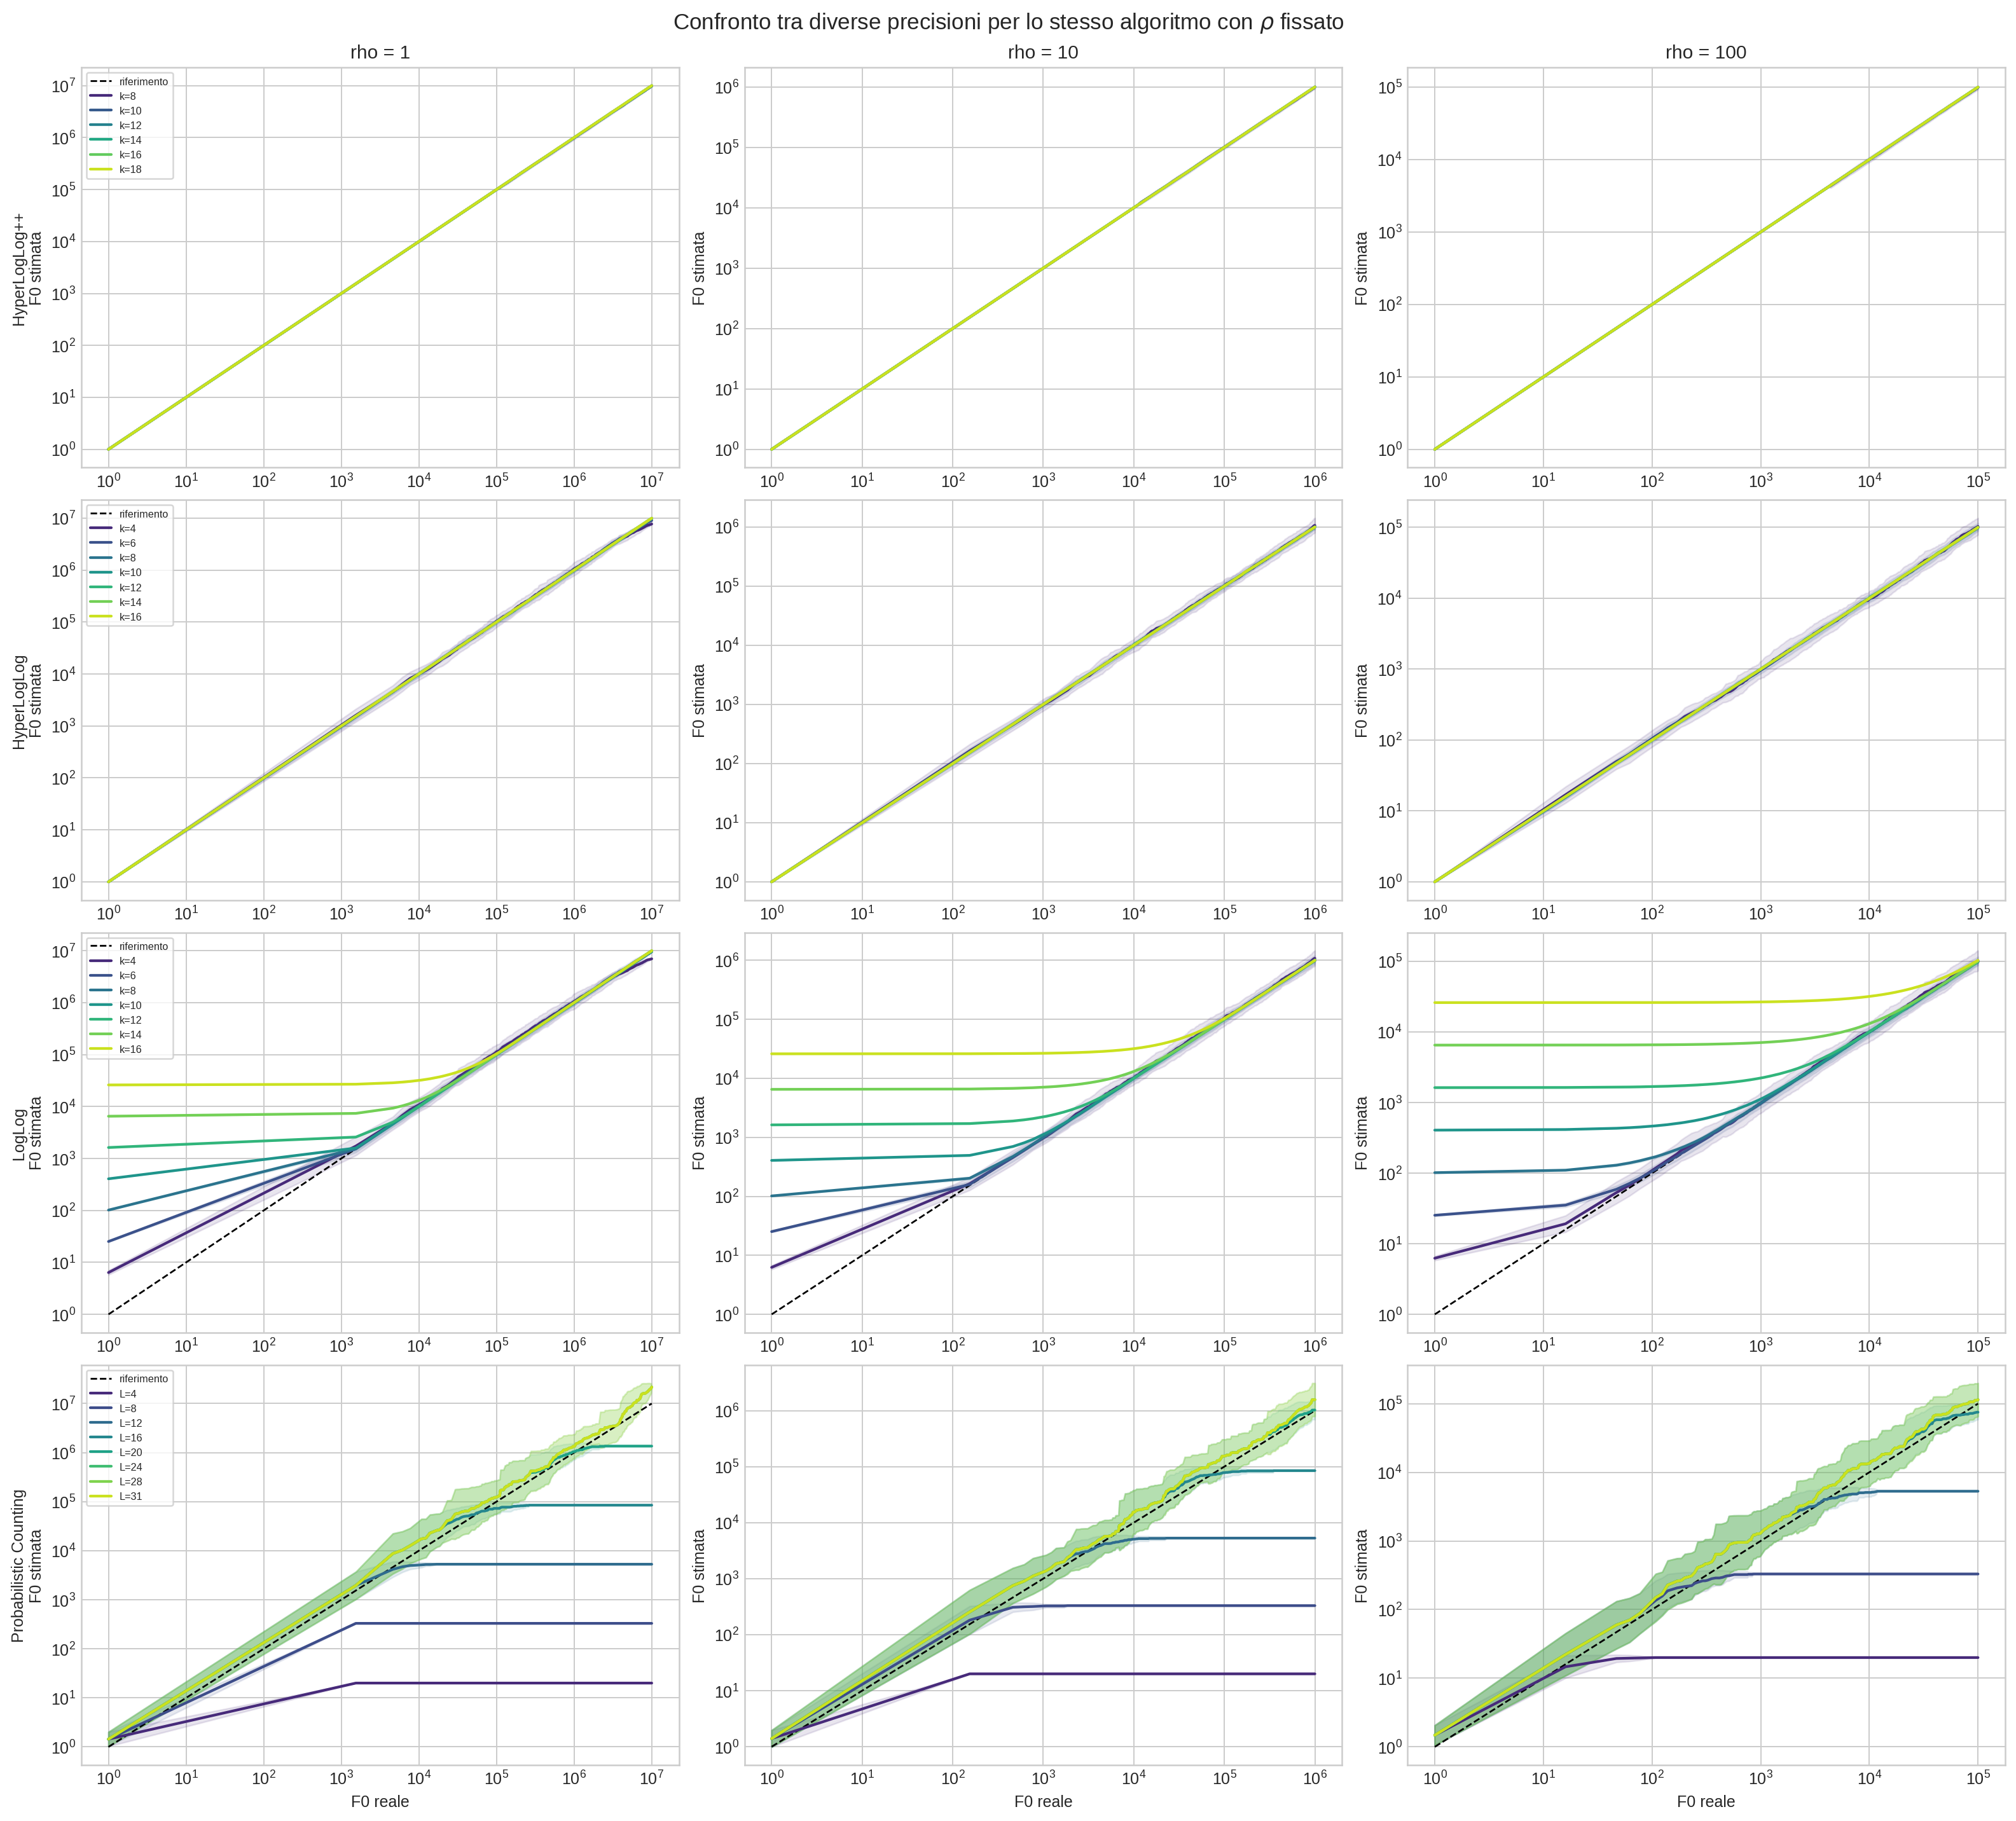
\includegraphics[height=0.33\textheight,keepaspectratio]{figures/results/streaming_precision_sweep_typeA_grid_loglog.png}
        \caption{Scala logaritmica}
        \label{fig:ch5-stream-precision-typea-loglog}
    \end{subfigure}
    \caption{Confronto rispetto alla cardinalità reale del prefisso nell'analisi del parametro di precisione. Le righe corrispondono agli algoritmi e le colonne ai tre valori di \(\rho\)}
    \label{fig:ch5-stream-precision-typea}
\end{figure}

\begin{table}[htbp]
    \centering
    \footnotesize
    \setlength{\tabcolsep}{4pt}
    \renewcommand{\arraystretch}{1.1}
    \begin{tabular}{|l|c|c|c|c|}
        \hline
        Algoritmo & Complessivo & \(\rho=1\) & \(\rho=10\) & \(\rho=100\) \\
        \hline
        HyperLogLog++ & \(k=18\) & \(k=18\) & \(k=18\) & \(k=18\) \\
        \hline
        HyperLogLog & \(k=16\) & \(k=10\) & \(k=16\) & \(k=16\) \\
        \hline
        LogLog & \(k=14\) & \(k=14\) & \(k=16\) & \(k=14\) \\
        \hline
        Probabilistic Counting & \(L=20\) & \(L=20\) & \(L=20\) & \(L=16\) \\
        \hline
    \end{tabular}
    \caption{Miglior parametro osservato per algoritmo nell'analisi del parametro di precisione}
    \label{tab:ch5-stream-precision-best}
\end{table}

\subsubsection{Risultati sulla precisione per ogni algoritmo}

Le Figure~\ref{fig:ch5-stream-precision-heatmaps} e
  \ref{fig:ch5-stream-precision-typea} mostrano che l'aumento del parametro di
  precisione non produce lo stesso effetto per tutti gli algoritmi.

  HyperLogLog++ \`e l'algoritmo con l'andamento pi\`u regolare. Nel dominio
  osservato, all'aumentare di \(k\) l'errore tende a ridursi in modo stabile e il
  valore migliore coincide sempre con \(k=18\), indipendentemente dal valore di
  \(\rho\). Questo comportamento indica che l'algoritmo non solo \`e accurato in
  media, ma risponde anche in modo prevedibile all'aumento delle risorse
  disponibili.

  HyperLogLog mostra una tendenza simile, ma meno uniforme. In media il parametro
  migliore \`e \(k=16\), tuttavia nel caso \(\rho=1\) il beneficio si stabilizza
  gi\`a attorno a \(k=10\). L'aumento del parametro continua quindi a migliorare
  la stima, ma con un guadagno meno regolare rispetto a HyperLogLog++.

  LogLog presenta invece un comportamento pi\`u irregolare. Il parametro migliore
  medio risulta \(k=14\), ma il vantaggio non cresce in modo monotono al crescere
  di \(k\): il valore \(k=16\) migliora il caso intermedio \(\rho=10\), ma non si
  mantiene ottimale negli altri regimi osservati. Questo suggerisce una maggiore
  sensibilit\`a alla scelta del parametro.

  Probabilistic Counting resta nettamente separato dagli altri algoritmi. Anche
  nel caso del parametro migliore, pari a \(L=20\), l'errore finale rimane molto
  pi\`u elevato e il miglioramento ottenuto aumentando \(L\) non \`e sufficiente a
  portare l'algoritmo su livelli comparabili con quelli delle famiglie a
  registri.

Questo esperimento aggiunge quindi un'informazione che i confronti precedenti
non mostravano direttamente. Non basta osservare quale algoritmo sia pi\`u
accurato nel complesso: \`e altrettanto importante capire se la qualit\`a della
stima migliori in modo regolare al variare del parametro. Sotto questo aspetto,
HyperLogLog++ risulta l'algoritmo pi\`u stabile e pi\`u robusto, mentre LogLog e
soprattutto Probabilistic Counting mostrano una dipendenza molto pi\`u marcata
dalla scelta del parametro. Anche questa evidenza è in linea con la dipendenza
classica dell'errore dal numero di registri, che nelle famiglie LogLog e
HyperLogLog segue un andamento dell'ordine di \(1/\sqrt{m}\)
\cite{Durand_Flajolet_2003,Flajolet_Fusy_Gandouet_Meunier_2007}.

\section{Esperimenti sul merge distribuito}
Tutti gli esperimenti sul merge sono stati fatti sull'algoritmo HyperLogLog++. 
Essi sono poi suddivisi secondo tre casi distinti:
\begin{itemize}
    \item \texttt{valid}: merge semanticamente corretto in modo diretto;
    \item \texttt{invalid}: merge non semanticamente corretto;
    \item \texttt{recoverable}: merge non direttamente corretto, ma
    recuperabile con normalizzazione esplicita.
\end{itemize}

La possibilità di costruire sketch locali e combinarli senza rivedere i dati
originari è uno dei motivi principali per cui queste strutture vengono usate in
contesti distribuiti e in sistemi che aggregano grandi collezioni di dataset
\cite{Agarwal_Cormode_Huang_Phillips_Wei_Yi_2012,Ting_2019_BillionsDatasets}.

La sperimentazione del merge omogeneo implementa il caso \texttt{valid}, 
mentre i due esperimenti
eterogenei permettono di osservare separatamente un caso \texttt{invalid} e un
caso \texttt{recoverable}.

 Nella lettura dei risultati eterogenei è utile osservare anche gli scenari
  invertiti tra lato sinistro e lato destro, indicati con il suffisso
  \texttt{rev}. Questa scelta non serve a verificare una nuova proprietà
  algebrica del merge eterogeneo, ma a controllare se il degrado osservato cambi
  quando si scambiano i due contesti locali. La proprietà matematica di
  commutatività del merge è invece già verificata nei test del caso omogeneo,
  insieme all'idempotenza e alla coerenza con il riferimento seriale.

\subsection{Caso omogeneo}
Affinch\'e si possa fare degli esperimenti nel caso di merge omogeneo, \`e
necessario effettuare il merge mantenendo identici la stessa funzione di hash, lo stesso seed
e gli stessi parametri dell'algoritmo.

La configurazione minima scelta prevede:
\[
\rho \in \{1,10,100\},\qquad
k \in \{10,14,18\}
\]
sono state analizzate 36 configurazioni e 900 coppie, combinando i tre valori
di \(k\), i tre regimi di \(\rho\) e le quattro funzioni di hash disponibili.

In tutte le 900 coppie analizzate si osserva:
\[
\Delta_{abs}=0,\qquad \Delta_{rel}=0
\]
La tabella seguente riassume lo stesso risultato nei tre regimi di \(\rho\)
considerati.

\begin{table}[htbp]
    \centering
    \small
    \setlength{\tabcolsep}{6pt}
    \renewcommand{\arraystretch}{1.1}
    \begin{tabular}{|r|r|r|r|r|r|r|}
        \hline
        \(\rho\) & \(d\) & Configurazioni & Coppie totali & Coppie con delta \(\neq 0\) & Max \(\Delta_{abs}\) & Max \(\Delta_{rel}\) \\
        \hline
        1 & \(10^7\) & 12 & 300 & 0 & 0 & 0 \\
        \hline
        10 & \(10^6\) & 12 & 300 & 0 & 0 & 0 \\
        \hline
        100 & \(10^5\) & 12 & 300 & 0 & 0 & 0 \\
        \hline
    \end{tabular}
    \caption{Risultati del controllo omogeneo di HyperLogLog++}
    \label{tab:ch5-merge-homo-summary}
\end{table}

Il controllo omogeneo costituisce il riferimento del caso \texttt{valid} e
mostra che, nel dominio osservato, merge e l'unione seriale coincidono in
modo sistematico. Questo esperimento fornisce quindi la base rispetto alla quale
leggere gli scostamenti osservati nei casi eterogenei. Il risultato è coerente
con la semantica classica del merge per gli sketch HLL-like, che in condizioni
omogenee coincide con lo stato ottenuto processando direttamente l'unione dei
flussi \cite{Ertl_2017_HLLAlgorithms}.

\subsection{Caso eterogeneo}

Nel caso di merge eterogeneo \`e stato deciso
di analizzare due precisi casi distinti. 
Lo scopo di questi esperimenti era cercare di analizzare quanto potesse degradare
il merge in condizioni non ottimali, come ad esempio in un contesto di nodi distribuiti,
in cui ogni nodo aveva a disposizione poca memoria e che fosse necessario utilizzare
precisioni o parametri differenti.

Il primo esperimento consiste nell'analisi sull'utilizzo di funzioni di hash differenti,
che rappresenta un caso \texttt{invalid}, mentre il
merge in caso di precisioni differenti appartiene ai casi \texttt{recoverable} e
richiede quindi una lettura diversa dei risultati.

\subsubsection{Hash mismatch}

  La prima analisi eterogenea riguarda il caso in cui i due sketch vengono
  costruiti usando funzioni di hash differenti, oppure la stessa famiglia di hash
  ma con seed diversi. L'obiettivo è capire come si comporti l'unione di sketch
  quando la semantica dell'hash non è più condivisa tra i due lati.

  Da questo esperimento ci si aspetta sicuramente una degradazione della stima. Poich\'e
  lo stesso numero rappresentato da due funzioni di hash differenti verr\`a rappresentato
  differentemente. L'esperimento vuole vedere quanto effettivamente viene degradata la stima.

  La configurazione considerata è stata:
  \[
  n=10^7,\qquad p=50,\qquad seed=21041998,\qquad
  d\in\{10^5,10^6,10^7\}
  \]
  da cui si ricava
  \[
  \rho\in\{100,10,1\}
  \]
  con precisione fissata a \(k=14\).

  Le funzioni di hash considerate in questa configurazione minima sono
  \texttt{splitmix64}, \texttt{xxhash64}, \texttt{murmurhash3} e
  \texttt{siphash24}. Gli scenari osservati sono sette:
  \begin{itemize}
      \item \texttt{ctrl}: controllo omogeneo locale, con la stessa funzione di
      hash sui due lati e seed del dataset su entrambi;
      \item \texttt{seed\_xx} e \texttt{seed\_xx\_rev}: stessa hash
      \texttt{xxhash64}, ma seed diversi nei due lati;
      \item \texttt{seed\_murmur} e \texttt{seed\_murmur\_rev}: stessa hash
      \texttt{murmurhash3}, ma seed diversi nei due lati;
      \item \texttt{family} e \texttt{family\_rev}: confronto tra
      \texttt{xxhash64} e una funzione di hash diversa tra
      \texttt{splitmix64}, \texttt{murmurhash3} e \texttt{siphash24}.
  \end{itemize}

  I casi di \emph{seed mismatch} sono stati testati solo su
  \texttt{xxhash64} e \texttt{murmurhash3}, perché in questa configurazione minima sono
  le due famiglie per cui l'utilizzo di seed differenti è stato usato come fattore
  di eterogeneità. Nei casi \texttt{family} e \texttt{family\_rev}, invece,
  l'eterogeneità riguarda direttamente l'utilizzo di funzioni di hash.

  Lo scenario \texttt{ctrl} è presente anche in questo esperimento come
  riferimento locale nella stessa figura e nella stessa tabella. Non rappresenta
  un esperimento distinto dal caso omogeneo discusso in precedenza, ma un suo
  sottoinsieme su HyperLogLog++ con \(k=14\), utile per confrontare direttamente
  i casi \texttt{invalid} con il comportamento corretto.

  Nel controllo omogeneo la strategia usata è \texttt{direct}. Nei casi
  \texttt{invalid}, invece, vengono osservate due strategie:
  \texttt{reject} e \texttt{unsafe\_naive\_merge}. La prima non produce una stima
  di merge e registra esplicitamente il caso incompatibile. La seconda forza il
  merge come se la coppia fosse compatibile, ed è quindi usata come controllo
  negativo sperimentale.

   Questo controllo serve quindi a distinguere i casi in cui il merge è trattato
  come semanticamente valido dai casi in cui viene forzato esplicitamente come
  controllo negativo.

  L'esperimento copre 1800 righe complessive, distribuite su 72 file in formato
  CSV:
  \begin{itemize}
      \item 300 coppie nel controllo omogeneo;
      \item 750 coppie \texttt{invalid} con \texttt{reject};
      \item 750 coppie \texttt{invalid} con \texttt{unsafe\_naive\_merge}.
  \end{itemize}

  La Figura~\ref{fig:ch5-hash-mismatch} mostra, per i diversi valori di \(\rho\),
  il contrasto tra il merge omogeneo locale e il merge forzato nei casi
  \texttt{invalid}. La Tabella~\ref{tab:ch5-hash-mismatch-summary} ne riassume i
  principali valori numerici. Le quantità \(\overline{\varepsilon}_{merge}\) e
  \(\overline{\varepsilon}_{serial}\) indicano rispettivamente l'errore relativo
  medio del merge e del riferimento seriale. La colonna finale riporta invece il
  degrado medio, cioè la media del rapporto punto per punto tra errore del merge
  ed errore del riferimento seriale.

  \begin{table}[htbp]
      \centering
      \small
      \setlength{\tabcolsep}{5pt}
      \renewcommand{\arraystretch}{1.1}
      \begin{tabular}{|l|r|r|r|r|r|}
          \hline
          Scenario & Coppie & \(\overline{\varepsilon}_{merge}\) & \(\overline{\varepsilon}_{serial}\) &
  \(\max \varepsilon_{merge}\) & Degrado medio \\
          \hline
          \texttt{ctrl} & 300 & 0.006233 & 0.006233 & 0.025913 & 1.00 \\
          \hline
          \texttt{seed\_xx} & 75 & 0.342374 & 0.007436 & 0.969548 & 49.45 \\
          \hline
          \texttt{seed\_xx\_rev} & 75 & 0.343830 & 0.010076 & 0.969548 & 28.82 \\
          \hline
          \texttt{seed\_murmur} & 75 & 0.347522 & 0.004836 & 0.984223 & 206.46 \\
          \hline
          \texttt{seed\_murmur\_rev} & 75 & 0.348319 & 0.004606 & 0.984223 & 307.18 \\
          \hline
          \texttt{family} & 225 & 0.352037 & 0.007436 & 1.009634 & 50.36 \\
          \hline
          \texttt{family\_rev} & 225 & 0.352802 & 0.005832 & 1.009634 & 130.76 \\
          \hline
      \end{tabular}
      \caption{Risultati del merge eterogeneo con funzioni di hash differenti}
      \label{tab:ch5-hash-mismatch-summary}
  \end{table}

    \begin{figure}[htbp]
      \centering
      \begin{subfigure}[t]{0.98\textwidth}
          \centering
          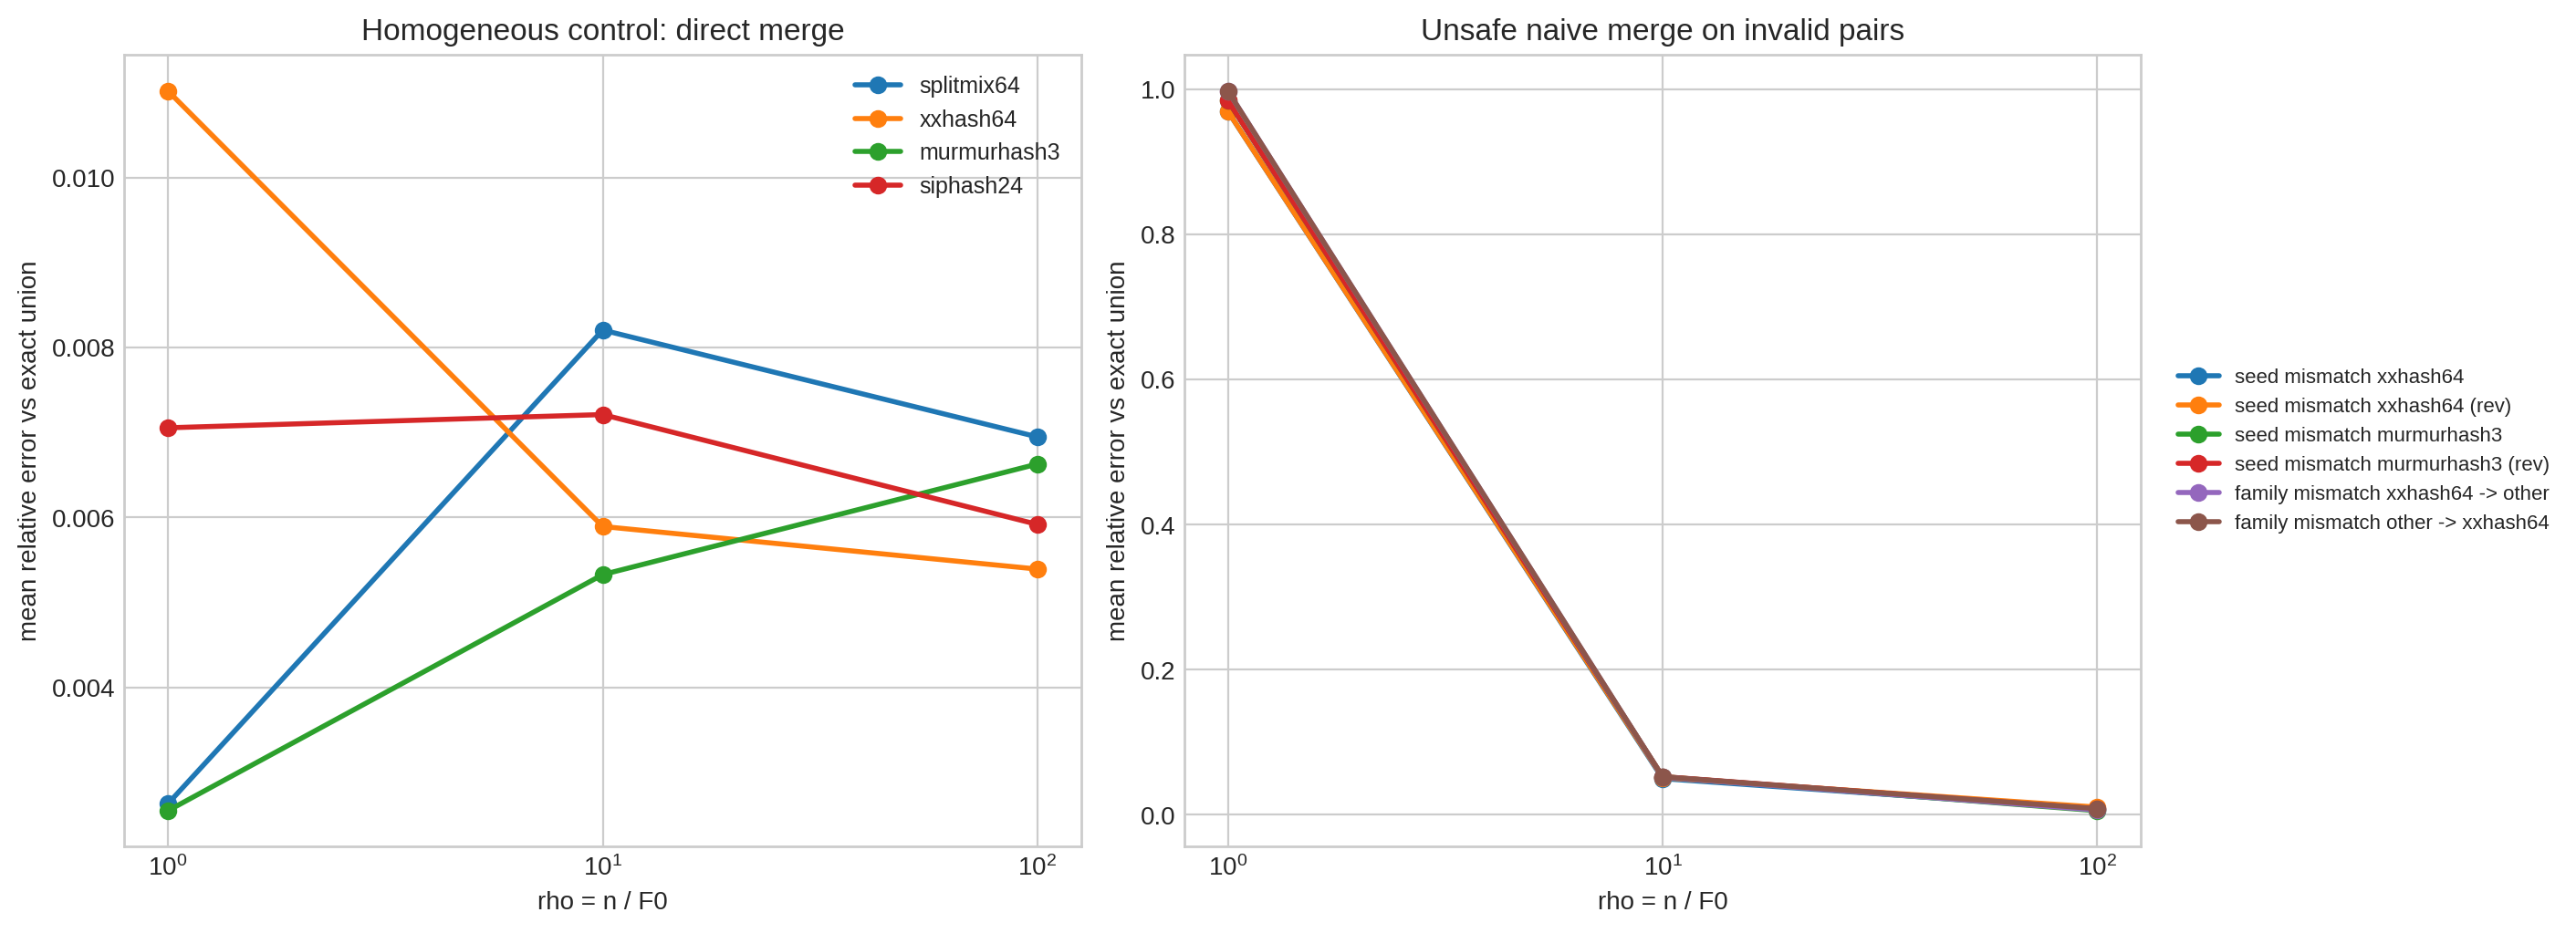
\includegraphics[width=\linewidth]{figures/results/merge_hpp_hash_mismatch_overview.png}
          \caption{Controllo omogeneo e andamento medio del merge forzato nei casi \texttt{invalid}}
          \label{fig:ch5-hash-mismatch-overview}
      \end{subfigure}
      \caption{Esperimento di merge eterogeneo con funzioni di hash differenti}
      \label{fig:ch5-hash-mismatch}
  \end{figure}

  Dai risultati emerge che, nei casi \texttt{invalid}, il merge forzato produce un
  degrado netto rispetto al riferimento seriale e conferma che l'eterogeneità
  dell'hash rompe la semantica comune necessaria al merge. Nel regime più
  critico, \(\rho=1\), l'errore relativo medio raggiunge valori prossimi o
  superiori a 1, con massimo pari a 1.009634. La strategia \texttt{reject}, al
  contrario, evita di trattare queste coppie come merge validi e mantiene nel
  protocollo sperimentale soltanto la stima seriale e l'unione esatta.

\subsubsection{Precision mismatch}

  La seconda analisi eterogenea riguarda l'esperimento in cui la funzione di hash resta
  costante, ma i due sketch vengono costruiti con precisioni differenti, cio\`e con parametri differenti
  per l'algoritmo, in questo caso cambia la quantit\`a di registri utilizzati.

  L'obiettivo è capire se l'utilizzo di parametri differenti rende il merge
  direttamente invalido oppure se il caso possa essere recuperato tramite una
  normalizzazione esplicita.

  La configurazione considerata è stata:
  \[
  n=10^7,\qquad p=50,\qquad seed=21041998,\qquad
  d\in\{10^5,10^6,10^7\}
  \]
  da cui si ricava
  \[
  \rho\in\{100,10,1\}
  \]
  con funzione di hash fissata a \texttt{xxhash64} e seed di hash identico sui
  due lati, pari a \(21041998\).

  Le coppie di precisione osservate sono:
  \[
  (k_{left},k_{right}) \in
  \{(10,14),(14,10),(10,18),(18,10),(14,18),(18,14)\}
  \]
  Questi sei casi vengono letti in tre gruppi di precisione:
  \texttt{10 vs 14}, \texttt{10 vs 18} e \texttt{14 vs 18}, ciascuno osservato
  nelle due direzioni tra lato sinistro e lato destro.

  In tutti questi casi la coppia è classificata come \texttt{recoverable}. Per
  questa ragione vengono osservate tre strategie:
  \texttt{reject}, \texttt{unsafe\_naive\_merge} e
  \texttt{reduce\_then\_merge}. La prima non produce una stima di merge e
  registra esplicitamente il caso. La seconda forza il merge senza alcuna
  normalizzazione preventiva. La terza riduce entrambi gli sketch alla precisione
  più bassa compatibile e applica poi il merge nello spazio comune.

  Questo controllo serve quindi a distinguere i casi in cui il parametro di precisione \`e differente
e che venga trattato come merge recuperabile dai casi in cui il
  merge viene forzato senza normalizzazione.

  L'esperimento copre 1350 righe complessive, distribuite su 54 file in formato
  CSV:
  \begin{itemize}
      \item 450 coppie \texttt{recoverable} con \texttt{reject};
      \item 450 coppie \texttt{recoverable} con \texttt{unsafe\_naive\_merge};
      \item 450 coppie \texttt{recoverable} con \texttt{reduce\_then\_merge}.
  \end{itemize}

  La Tabella~\ref{tab:ch5-precision-mismatch-summary} riassume i principali
  valori numerici dell'esperimento. Le quantità
  \(\overline{\varepsilon}_{merge}\) e \(\overline{\varepsilon}_{serial}\)
  indicano rispettivamente l'errore relativo medio del merge e del caso
  seriale. Anche in questo caso l'ultima colonna riporta il degrado medio, cioè
  la media del rapporto punto per punto tra errore del merge ed errore del
  merge seriale. La riga \texttt{reject} non corrisponde a una stima di
  merge, ma a una strategia di rifiuto; per questo le colonne relative al merge
  restano non valorizzate.

  \begin{table}[htbp]
      \centering
      \small
      \setlength{\tabcolsep}{5pt}
      \renewcommand{\arraystretch}{1.1}
      \begin{tabular}{|l|r|r|r|r|r|}
          \hline
          Strategia & Coppie & \(\overline{\varepsilon}_{merge}\) & \(\overline{\varepsilon}_{serial}\) & \(\max
  \varepsilon_{merge}\) & Degrado medio \\
          \hline
          \texttt{reject} & 450 & -- & 0.016651 & -- & -- \\
          \hline
          \texttt{unsafe\_naive\_merge} & 450 & 0.363882 & 0.016651 & 1.061378 & 32.37 \\
          \hline
          \texttt{reduce\_then\_merge} & 450 & 0.016651 & 0.016651 & 0.057418 & 1.00 \\
          \hline
      \end{tabular}
      \caption{Risultati del merge eterogeneo nel caso in cui i parametri degli algoritmi non coincidono}
      \label{tab:ch5-precision-mismatch-summary}
  \end{table}

  \begin{figure}[htbp]
      \centering
      \begin{subfigure}[t]{0.98\textwidth}
          \centering
          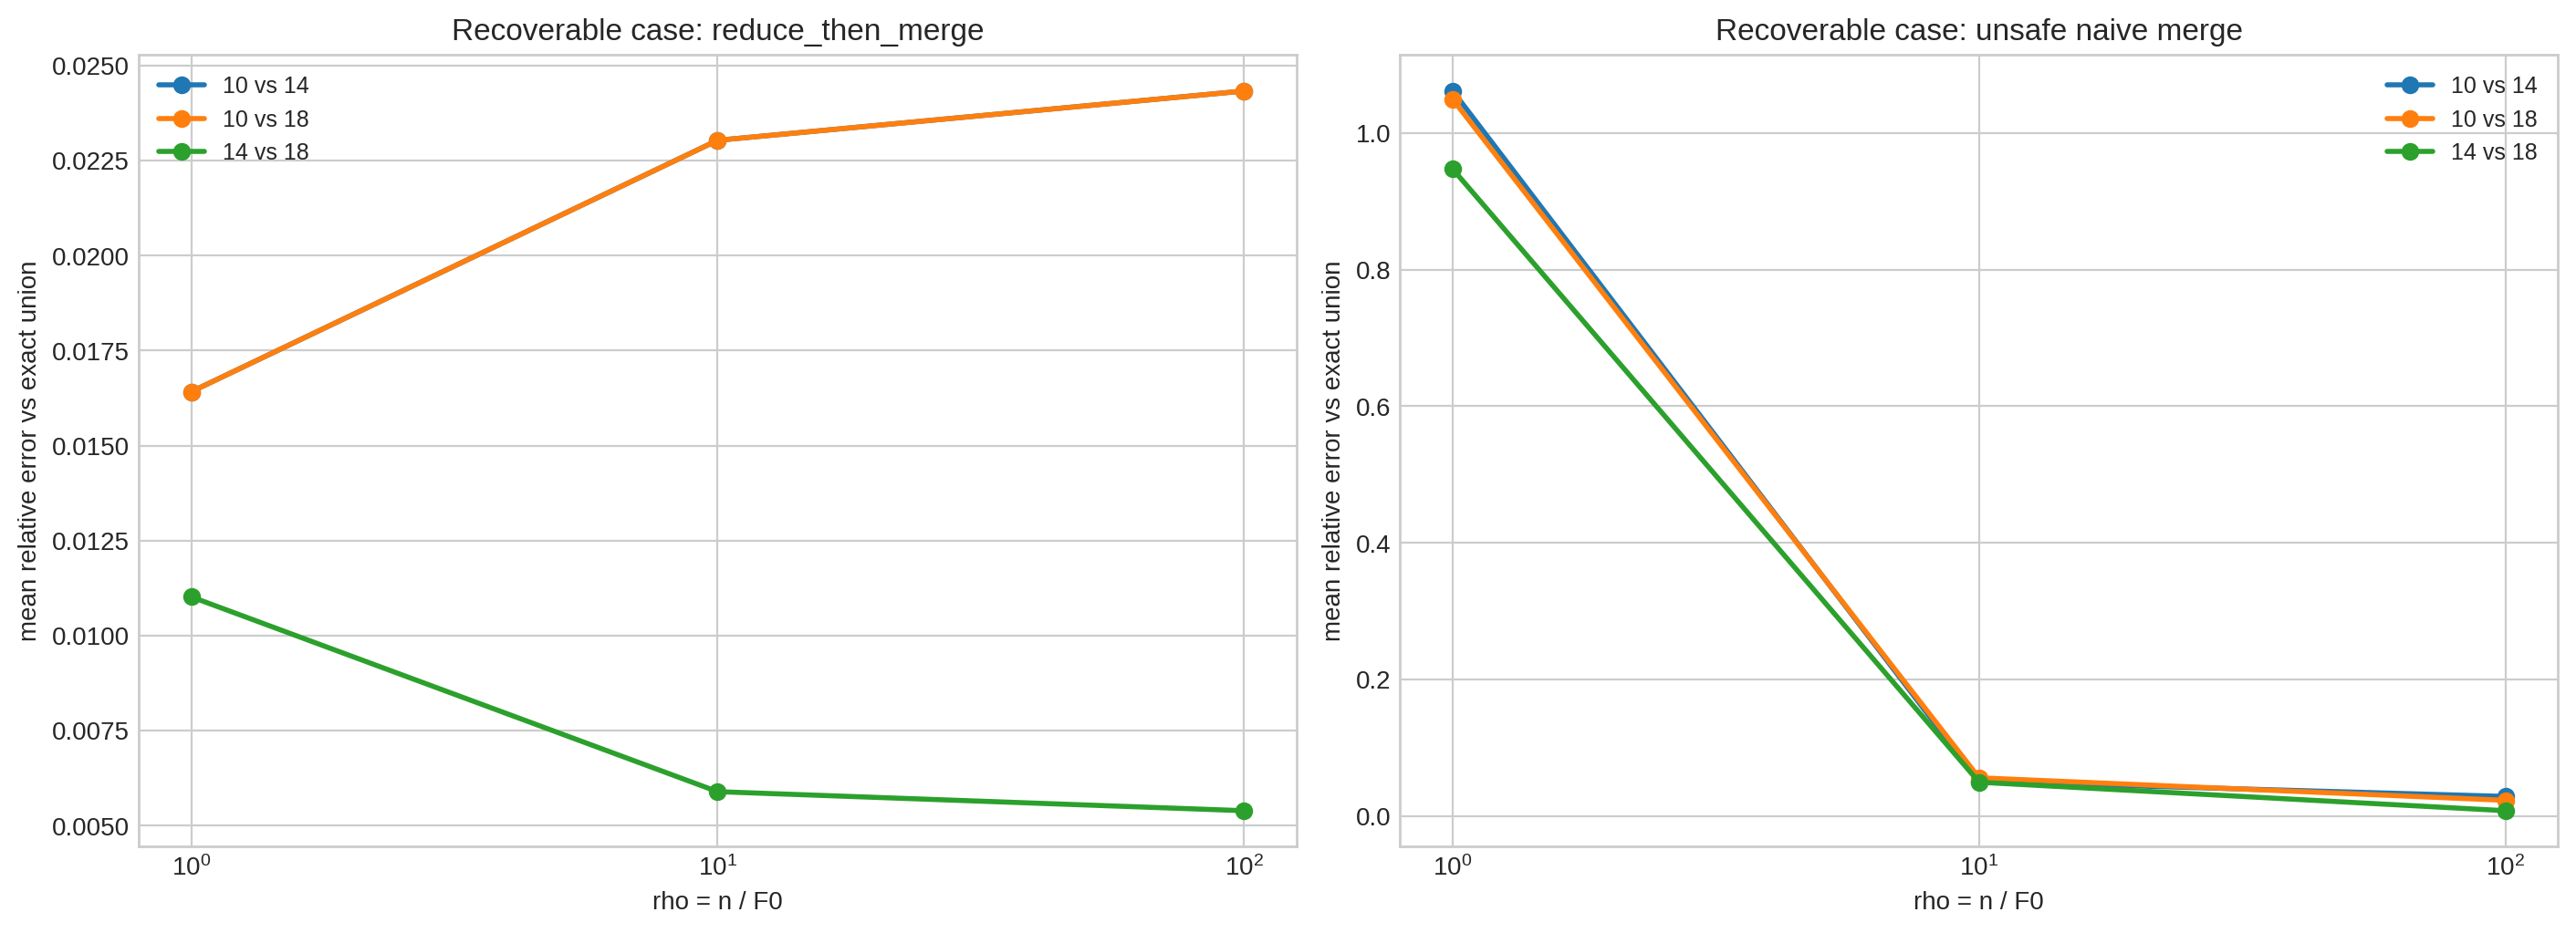
\includegraphics[width=\linewidth]{figures/results/merge_hpp_precision_mismatch_overview.png}
          \caption{Confronto tra \texttt{reduce\_then\_merge} e \texttt{unsafe\_naive\_merge} nel caso in cui i parametri degli algoritmi non coincidono}
          \label{fig:ch5-precision-mismatch-overview}
      \end{subfigure}
  \end{figure}

  \paragraph{Correttezza della normalizzazione \texttt{reduce\_then\_merge}}

  Dai risultati emerge che, nei casi \texttt{recoverable}, la normalizzazione alla
  precisione minima elimina lo scostamento introdotto dall'utilizzo di parametri differenti. 
  Con l'utilizzo della strategia \texttt{reduce\_then\_merge}, il comportamento coincide infatti
  sia con il riferimento seriale sia con il riferimento omogeneo alla precisione
  più bassa, con degrado medio pari a \(1.00\). Questo comportamento è coerente
  con la letteratura più recente sugli sketch HyperLogLog, che tratta la
  riduzione alla precisione minima come passaggio corretto per rendere
  confrontabili sketch costruiti con parametri diversi
  \cite{Ertl_2017_HLLAlgorithms}.

  \paragraph{Degrado del merge forzato nel caso \texttt{recoverable}}

  Quando la normalizzazione non viene applicata, il merge forzato mostra invece un
  degrado netto rispetto al riferimento seriale. Nel gruppo \texttt{10 vs 14},
  l'errore relativo medio passa da circa \(0.0290\) per \(\rho=100\) a
  \(0.0509\) per \(\rho=10\), fino a raggiungere \(1.061378\) per \(\rho=1\).
  Nel gruppo \texttt{10 vs 18} i valori sono molto simili, con massimo
  \(1.049045\) nel regime \(\rho=1\). Nel gruppo \texttt{14 vs 18} il degrado
  resta più contenuto per \(\rho=100\), ma cresce nuovamente fino a
  \(0.947067\) quando \(\rho=1\). Anche in questo caso, quindi, il merge forzato
  non si limita a introdurre una perdita moderata di accuratezza, mentre la
  strategia \texttt{reduce\_then\_merge} riporta il comportamento al riferimento
  corretto.

\section{Risultati ottenuti}

I risultati presentati in questo capitolo possono essere riassunti in quattro
punti principali.

\begin{itemize}
    \item \textbf{Algoritmo migliore: HyperLogLog++.} Nel dominio sperimentale
    osservato, HyperLogLog++ risulta il metodo migliore perché combina
    \textit{accuratezza media più alta}, \textit{minore dispersione della
    stima} e \textit{comportamento più regolare al variare del parametro di
    precisione}. Le Figure~\ref{fig:ch5-stream-f0-hll},
    \ref{fig:ch5-stream-rho-hll} e
    \ref{fig:ch5-stream-endpoint-summary} mostrano infatti che HyperLogLog++
    mantiene la stima più stabile sia rispetto alla cardinalità reale del
    prefisso sia rispetto al rapporto tra elementi processati e distinti. La
    Tabella~\ref{tab:ch5-stream-precision-best} conferma inoltre che, durante l'esperimento sui possibili parametri,
    HyperLogLog++ è anche l'algoritmo con la risposta più
    prevedibile all'aumentare di \(k\), con valore migliore osservato sempre pari
    a \(k=18\).

    \item \textbf{Coincidenza tra merge omogeneo e riferimento seriale.} Quando
    due sketch condividono la stessa funzione di hash, lo stesso seed e gli
    stessi parametri, il merge coincide con il caso seriale nel dominio
    osservato. La Tabella~\ref{tab:ch5-merge-homo-summary} riporta infatti
    \(\Delta_{abs}=0\) e \(\Delta_{rel}=0\) in tutte le coppie analizzate.
    Questo è il risultato di riferimento del caso \texttt{valid} e mostra che,
    in condizioni omogenee, il merge preserva correttamente la semantica dello
    sketch.

    \item \textbf{Hash diverse nel merge compromettono la correttezza.} Quando
    i due sketch sono costruiti con funzioni di hash diverse, oppure con seed
    diversi della stessa famiglia di hash, il merge produce un degrado
    netto rispetto al riferimento seriale. La
    Tabella~\ref{tab:ch5-hash-mismatch-summary} mostra che l'errore relativo
    medio del merge cresce di oltre un ordine di grandezza e, nel regime più
    critico \(\rho=1\), può superare il valore \(1\). Questo conferma che il
    merge richiede non solo lo stesso algoritmo, ma anche una semantica comune
    dell'hash.

    \item \textbf{La tecnica \texttt{reduce\_then\_merge} recupera il caso di
    precisioni diverse.} Se i due sketch usano la \textit{stessa funzione di
    hash} ma \textit{precisioni diverse}, il merge non è direttamente corretto,
    ma può essere recuperato normalizzando entrambi gli sketch alla precisione
    minima comune prima dell'unione. La
    Tabella~\ref{tab:ch5-precision-mismatch-summary} mostra che, con
    \texttt{reduce\_then\_merge}, l'errore medio del merge coincide con quello
    del riferimento seriale e del corrispondente caso omogeneo, mentre il merge
    senza normalizzazione introduce un degrado netto.
\end{itemize}

Complessivamente, il risultato principale del capitolo è che HyperLogLog++
emerge come il miglior stimatore tra quelli implementati, mentre sul lato del
merge la correttezza dipende in modo decisivo dalla compatibilità semantica tra
gli sketch: il caso omogeneo coincide con il seriale, l'eterogeneità dell'hash
rompe la correttezza, e quando due sketch hanno precisioni diverse il merge resta recuperabile solo
attraverso una normalizzazione esplicita.

    \chapter{Conclusioni}
\label{chp:conclusioni}

Volendo idea: sarebbe da prendere i dati in una stream continua e fare misurazione real-time di quello che
accade, ovviamente non si può sapere il valore esatto in questo caso.

Però si potrebbe invece fare che la stream esiste già però vengono dati un valore alla volta, in modo tale
da avere effettivamente i valori.

Pensare anche all'implementazione di un sistema reale di streaming di dati come Apache Kafka.

    
    % afterword
    \cleardoublepage
    \phantomsection
    \addcontentsline{toc}{chapter}{Bibliografia}
    \bibliography{references.bib}

\end{document}
